\documentclass[a4paper,11pt]{report}

\usepackage[a4paper]{geometry}
% Lingua documento
\usepackage[italian]{babel}
\usepackage[T1]{fontenc} 
\usepackage[utf8]{inputenc}
% Pacchetti per la matematica
\usepackage{amsmath}
\usepackage{amsfonts}
\usepackage{amssymb}
\usepackage{gensymb}
\usepackage{braket}

\usepackage{cases}
\usepackage{enumitem}
\usepackage{graphicx}

\newcommand{\vect}[1]{\boldsymbol{#1}}
\setlength{\parindent}{0cm}

\title{Appunti del corso di Equazioni Differenziali I}
\author{raccolti da \\Luca Colombo Gomez}
\date{AA 2017/2018}

\newcommand{\R}{\mathbb{R}}
\newcommand{\Rn}{\mathbb{R}^n}
\newcommand{\x}{\boldsymbol{x}}
\newcommand{\xp}{\boldsymbol{x}'}
\newcommand{\y}{\boldsymbol{y}}
\newcommand{\yp}{\boldsymbol{y}'}
\newcommand{\kk}{\boldsymbol{k}}
\newcommand{\kp}{\boldsymbol{k}'}
\newcommand{\z}{\boldsymbol{z}}
\newcommand{\n}{\boldsymbol{n}}

\makeindex

\begin{document}
\titlepage
\maketitle

\tableofcontents
\chapter{Parentesi matematica: distribuzioni e trasformate di Fourier}
\section{Distribuzioni}

Le \emph{distribuzioni} (o \emph{funzioni generalizzate}) sono degli oggetti che generalizzano le funzioni e le distribuzioni di probabilit\`a.
Estendono il concetto di derivata a tutte le funzioni continue e oltre.
Le distribuzioni sono importanti in fisica (p.e. distribuzione delta di Dirac).

\medskip
Idea di base:
\[
f:\R\rightarrow\R \text{ funzione integrabile}
\]
\[
\phi : \R \rightarrow \R \text{ smooth $\left(C^{\infty}\right)$, con supporto compatto} 
\]

\emph{Supporto compatto}, cio\'e identicamente zero tranne in un insieme compatto.

\smallskip

$\Rightarrow \int f \phi \, dx \in \mathbb{R}$, dipende linearmente e in un modo continuo da $\phi$.

\smallskip

$\Rightarrow f$ \`e un funzionale lineare continuo sullo spazio di tutte le \emph{funzioni test} $\phi.$

\smallskip

Questa \`e la definizione di una distribuzione.

Le distribuzioni possono essere moltiplicate con dei numeri reali, e possono essere sommate $\rightarrow$ formano uno spazio vettoriale reale.

\paragraph{Derivata di una distribuzione}

Considera prima il caso di una funzione $f:\R \rightarrow \R$ differenziabile. Se $\phi$ \`e una funzione test, abbiamo:
\[
\int_{\R}f'\phi \,dx = -\int_{\R}f\phi ' \,dx
\]
non c'\`e un termine di bordo perch\'e $\phi $ ha supporto compatto. 
Questo suggerisce la seguente definizione della derivata $S'$ di una distribuzione $S$:

$S'$ \`e funzionale lineare che manda la funzione test $\phi$ in $-S\left(\phi'\right)$

\subsection{Delta di Dirac}
La \emph{funzione delta di Dirac} \`e la distribuzione che manda la funzione test $\phi$ in $\phi(0)$. \`E la derivata della funzione step di Heaviside.
\[
H(x)=\begin{cases}
0 & x < 0 \\
1 & x \geq 0
\end{cases}
\]

La derivata della delta di Dirac \`e la distribuzione che manda $\phi$ in $-\phi '(0)$. La delta \`e un esempio di una distribuzione che non \`e una funzione, ma pu\`o essere definita come limite di una sequenza di funzioni, p.e.
\[
\delta\left(x\right) = \lim_{a\to 0}\delta_a\left(x\right)
\]
\[
\delta_a(x) = \begin{cases}
\frac{1}{2a} & -a\leq x\leq a\\
0 & |x| > a
\end{cases}
\]

\begin{center}
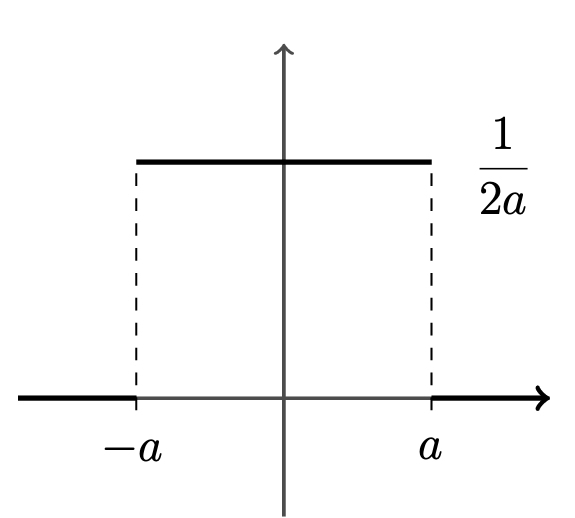
\includegraphics[width=0.4\textwidth]{immagini/grafico1}
\end{center}

\underline{Dimostrazione}:

\[
\int_\R \delta_a (x)\phi(x) dx= \int_{-a}^{a}\frac{1}{2a}\phi(x) dx = \frac{1}{2a}\big(\varphi(a)-\varphi(-a)\big)
\]
dove $\varphi$ \`e la primitiva di $\phi$, $\varphi'(x)=\phi(x)$

\[
\Rightarrow \lim_{a\to 0}\int_{\R}\delta_a(x)\phi(x)dx=\lim_{a\to 0}\frac{\varphi(a)-\varphi(-a)}{2a}=\varphi'(0)=\phi(0) \qquad\blacksquare
\]

\bigskip

\underline{Definizione}: Una funzione $\phi : U \rightarrow \mathbb{R}$ ($U\subseteq \Rn$) ha \emph{supporto compatto} se esiste un sottoinsieme compatto $K$ di $U$ tale che $\phi(\x)=0$ $\forall \x \in U\smallsetminus K$.

Le funzioni $C^{\infty}$ $\phi :U\rightarrow \mathbb{R}$ con supporto compatto formano uno spazio vettoriale reale $D(U)$.

\medskip

\underline{Definizione}: Lo \emph{spazio delle distribuzioni} su $U \subseteq \mathbb{R}^n$ \`e il duale $D\sp\prime(U)$ dello spazio vettoriale $D(U)$ di funzioni $C^{\infty}$ con supporto compatto in $U$.

Notazione: 
\[
S \in D\sp\prime(U), \qquad
\phi \in D(U), \qquad
S : D(U)\rightarrow \mathbb{R}, \qquad 
\phi \mapsto S(\phi) = \Braket{S,\phi}
\]

Una funzione integrabile $f$ definisce una distribuzione $\tilde{f}$ su $\mathbb{R}^n$ tramite:
\begin{equation}
\Braket{\tilde{f},\phi} := \int_{\Rn} f \phi \,d^{n}\x, \quad\forall \phi \in D(U) 
\end{equation}

Si dice che $\tilde{f}$ \`e la distribuzione associata alla funzione $f$, o che la distribuzione $\tilde{f}$ \`e equivalente alla funzione $f$.

La distribuzione di Dirac (o misura di Dirac) \`e definita da 
\begin{equation}
\Braket{\delta,\phi} := \phi(0) 
\end{equation}

\underline{Teorema}: La distribuzione di Dirac non pu\`o essere rappresentata da una funzione integrabile. 

\underline{Dimostrazione}: vedi \emph{Analysis, manifolds, and physics}, Choquet-Bruhat et al., p. 438. 

\medskip

Nonostante ci\`o scriveremo in seguito formalmente che:
\begin{equation}
\Braket{\delta , \phi} = \int_{\Rn} \delta (\x) \phi(\x) d^n \x= \phi(0) 
\end{equation}

\underline{Esercizio}: ($ \mathbb{R}^n$, $n=1$) Si dimostri che:
\begin{equation}
\delta' (x) =-\frac{\delta(x)}{x}
\end{equation}
Si ha:
\[
\int x\delta(x)\phi(x)dx = x\phi(x)\Big|_{x=0}=0 \quad \forall \phi \Rightarrow x\delta(x)=0
\]
Facciamo formalmente la derivata usando la regola di Leibniz:
\[
\Rightarrow \delta(x) + x\delta'(x)=0 \Rightarrow \delta ' (x) = -\frac{\delta(x)}{x}  \qquad \blacksquare
\]

Un'altra identit\`a utile \`e:
\begin{equation}
\delta\big(g(x)\big) = \sum_{i}\frac{\delta(x-x_i)}{|g'(x_i)|} 
\end{equation} 
dove $x_i$ sono gli zeri della funzione $g(x)$.

\underline{Dimostrazione}: la dimostrazione \`e lasciata allo studente.

Hint:
\begin{itemize}
\item Considera intorni che contengono un solo zero di $g(x)$
\item Riscrivi l'integrale come sommatoria
\item Applica la $\delta\big(g(x)\big)$ alla funzione di test $\phi$
\end{itemize}

\paragraph{Rappresentazione della delta}
\[
\delta(x) = \lim_{a\to 0} \delta_a(x),
\]
con 
\begin{subequations}
\begin{equation}
\delta_a(x)=\begin{cases}
\frac{1}{2a} & -a \leq x \leq a \\
0 & |x| > a
\end{cases}
\label{1.6a}
\end{equation}
\begin{equation}
\delta_a(x) = \frac{1}{\pi}\frac{a}{a^2+x^2}
\label{1.6b}
\end{equation}
\begin{equation}
\delta_a(x) = \frac{1}{a\sqrt{\pi}} e^{-\frac{x^2}{a^2}}
\label{1.6c}
\end{equation}
\begin{equation}
\delta_a(x) = \frac{1}{2\pi} \int_{-\infty}^{+\infty} e^{ikx-a|k|}dk
\label{1.6d}
\end{equation}
\end{subequations}

\underline{Dimostrazione} della \eqref{1.6b}:
\[
\int_{-\infty}^{+\infty} \delta_a(x)\phi(x)dx=\frac{1}{\pi}\int_{-\infty}^{+\infty}\frac{a}{a^2+x^2}\phi(x)dx \overset{x=at}{=} \frac{1}{\pi}\int_{-\infty}^{+\infty}\frac{1}{1+t^2}\phi(at)dt
\]
\[
\lim_{a\to 0} \int_{-\infty}^{+\infty}\delta_a(x)\phi(x)dx=\frac{1}{\pi}\lim_{a\to 0}\int_{-\infty}^{+\infty}\phi(at)\frac{dt}{1+t^2}
\]

Usa il \emph{teorema della convergenza dominata}:

Se $\{f_k\}_{k\in\mathbb{N}}$ \`e una successione di funzioni misurabili con limite puntuale $f$, e se esiste una funzione integrabile $g$ tale che $|f_k|\leq g \; \forall k$ allora $f$ \`e integrabile e
\[
\lim_{k\to \infty}\int f_k(x) dx = \int f(x) dx
\]

Da noi $f_k(t)\hat{=}\frac{\phi(at)}{1+t^2}$

$\rightarrow$ funzione $g$ esiste, perch\'e $\phi$ ha supporto compatto.

Quindi:
\[
\lim_{a\to 0}\int_{-\infty}^{+\infty}\delta_a(x)\phi(x)dx=\frac{1}{\pi}\int_{-\infty}^{+\infty} \lim_{a\to 0} \phi(at) \frac{dt}{1+t^2}=\frac{1}{\pi} \phi(0) \arctan{(t)}\Big|_{-\infty}^{+\infty}=\phi(0) \qquad \blacksquare
\]

Le dimostrazioni della \eqref{1.6c} e \eqref{1.6d} sono lasciate allo studente.

Hint:
\begin{itemize}
\item Calcola $\lim_{a\to 0}\int_{-\infty}^{+\infty}\delta_a(x)\phi(x)dx$ e usa il teorema della convergenza dominata (fai l'opportuno cambio di variabili)
\item $\frac{1}{2\pi}\int^{+\infty}_{-\infty} e^{ikx-a|k|}dk = \frac{1}{\pi}\frac{a}{a^2+x^2}$ 
\end{itemize}

\medskip

In $N$ dimensioni: coordinate cartesiane $x_1,x_2,\dots,x_n \Rightarrow \delta(\x)= \delta(x_1)\dots \delta(x_n)$

\medspace

Propriet\`a utili della delta di Dirac:
\[
\delta(-\boldsymbol{r})=\delta(\boldsymbol{r})
\]
\begin{equation}
\int_{\R^n} d^n\vect{r}\,\delta(\underbrace{\vect{r}-\vect{r}'}_{:=\vect{\rho}})f(\boldsymbol{r}) =
\int_{\R^n}d^n\vect{\rho}\,\delta(\vect{\rho})f(\vect{\rho}+\vect{r}')=
f(\vect{\rho}+\vect{r}')\Big |_{ \vect{\rho}=0}  = f(\vect{r}')
\label{1.7}
\end{equation}
Scegli $f=1$ $\Rightarrow$ formalmente 
\begin{equation}
\int_{\R^n}d^n\vect{r}\delta(\vect{r}-\vect{r}')=1
\end{equation}

\medspace

Delta di Dirac in coordinate curvilinee:

La quantit\`a invariante per trasformazione di coordinate \`e: $d^n\vect{r}\,\delta(\vect{r}-\vect{r}')$

Coordinate: $\xi_i (x_i,\dots,x_n)$, $i=1,\dots,n$, $x_j$ sono le coordinate cartesiane

Jacobiano
\[
J(x_i,\xi_j)=\left(\begin{matrix}
\frac{\partial x_1}{\partial \xi_1} & \dots & \frac{\partial x_1}{\partial \xi_n}\\
\vdots & & \vdots \\
\frac{\partial x_n}{\partial \xi_1} & \dots &\frac{\partial x_n}{\partial \xi_n}
\end{matrix}\right)dx_1\dots dx_n \delta(x_1-x_1')\dots \delta(x_n - x_n')=
\]
\[
=|J|d\xi_1\dots d\xi_n \delta(x_1 - x_1')\dots \delta(x_n-x_n')=
\]
\[
\overset{!}{=}d\xi_1 \dots d\xi_n\delta(\xi_1\dots \xi_1')\dots \delta(\xi_n - \xi_n')
\]
dove $|J|$ \`e il modulo del determinante del Jacobiano.
\begin{equation}
\Rightarrow\delta(\xi_1-\xi_1')\dots\delta(\xi_n-\xi_n')=|J|\delta(x_1-x_1')\dots\delta(x_n-x_n')
\end{equation}

\underline{Esempio}: Coordinate sferiche in 3 dimensioni:
\[
\begin{cases}
x=r\cos\varphi\sin\theta \\
y=r\sin\varphi\sin\theta \\
z=r\cos\theta
\end{cases}
\qquad
\begin{cases}
\xi_1=r \\
\xi_2=\theta \\
\xi_3=\varphi
\end{cases}
\]
Scrivo il Jacobiano e ne calcolo il determinante:
\[
\left|\frac{\partial x_i}{\partial \xi_j}\right|=\left|\begin{matrix}
\frac{\partial x}{\partial r} & \frac{\partial x}{\partial \theta} & \frac{\partial x}{\partial \varphi} \\
\frac{\partial y}{\partial r} & \frac{\partial y}{\partial \theta} & \frac{\partial y}{\partial \varphi}\\
\frac{\partial z}{\partial r} & \frac{\partial z}{\partial \theta} & \frac{\partial z}{\partial \varphi}
\end{matrix}\right|=r^2\sin\theta
\]
\begin{equation}
\Rightarrow \delta(r-r')\delta(\theta - \theta')\delta(\varphi - \varphi') = r^2\sin\theta \delta(x-x')\delta(y-y')\delta(z-z')
\end{equation}

\underline{Esempio}: Coordinate cilindriche in 3 dimensioni:
\[
\begin{cases}
x=r\cos\theta \\
y=r\sin\theta \\
z=z
\end{cases}
\qquad
\begin{cases}
\xi_1=r \\
\xi_2=\theta \\
\xi_3=z
\end{cases}
\]
Scrivo il Jacobiano e ne calcolo il determinante:
\[
\left|\frac{\partial x_i}{\partial \xi_j}\right|=\left|\begin{matrix}
\frac{\partial x}{\partial r} & \frac{\partial x}{\partial \theta} & \frac{\partial x}{\partial z} \\
\frac{\partial y}{\partial r} & \frac{\partial y}{\partial \theta} & \frac{\partial y}{\partial z}\\
\frac{\partial z}{\partial r} & \frac{\partial z}{\partial \theta} & \frac{\partial z}{\partial z}
\end{matrix}\right|=r
\]
\[
\Rightarrow \delta(r-r')\delta(\theta - \theta')\delta(z - z') = r \delta(x-x')\delta(y-y')\delta(z-z')
\]

\medskip

\emph{Densit\`a di carica} di un insieme discreto di $N$ cariche puntiformi:
\begin{equation}
\rho(\vect{r}) = \sum_{i=1}^{N} q_i\delta(\vect{r}-\vect{r}_i)
\label{1.11}
\end{equation}

\underline{Esercizio}: Si usi la \eqref{1.11} in
\[
\vect{E}(\vect{r})=\int d^3\vect{r}'\rho(\vect{r}')\frac{\vect{r}-\vect{r}'}{|\vect{r}-\vect{r}'|^3}
\]
e dimostrare usando la \eqref{1.7} che in un sistema di cariche puntiformi
\[
\vect{E}(\vect{r})= \sum_{i=1}^{N} q_i\frac{\vect{r}-\vect{r}_i}{|\vect{r}-\vect{r}_i|^3}
\]

\underline{Esempio}: Carica $Q$ uniformemente distribuita su una superficie sferica con raggio $R$. 
Determinare $\rho(\vect{r})$

Chiamo $\rho(\vect{r})=A Q\delta(r-R)$ con $A$ da determinare.
\[
\int d^3\vect{r}\rho(\vect{r})= \int dr d\theta d\phi \, r^2 \sin\theta  A Q \delta(r-R) = 4\pi AQ \int dr \, r^2 \delta(r-R)=4\pi AQR^2
\]
Normalizzando $4\pi AQR^2 =Q$ ottengo $A=\frac{1}{4\pi R^2}$
\[
\rho(\vect{r})=\frac{Q}{4\pi R^2}\delta(r-R)
\]

\section{Trasformata di Fourier}

\underline{Definizione}: 
Sia $X$ uno spazio di misura con misura $m$ positiva (possiamo prendere la misura di Lebesgue come esempio).
Definiamo gli \emph{spazi} $L^P$ come:

$L^P(X):=$ spazio di funzioni su $X$ tale che $|f|^p$ sia integrabile, $\int_{X}|f|^p dm < \infty$

Si dimostra che per $p\geq1$, $L^P(X)$ \`e uno spazio vettoriale e 
\[
\left\|f\right\| := \left( \int_{X} |f|^p dm\right)^{\frac{1}{p}}
\]
\`e una norma su questo spazio.

A noi interessa il caso in cui $m$ \`e la misura di Lebesgue; in tal caso gli elementi di $L^P(X)$ sono le funzioni $f$ con 
\[
\int_{X}|f|^p dx < \infty
\]

Il caso p=2 trova applicazioni in meccanica quantistica.

\medskip

\underline{Definizione}: Sia $f\in L^1 (\Rn)$, la \emph{trasformata di Fourier} $\mathcal{F}f$ \`e una funzione in $\Rn$ (in realt\`a sul duale di $\R^n$, identificato con $\R^n$) definita da:
\begin{equation}
\left( \mathcal{F} f\right)(\vect{k}) = \int_{\Rn}e^{-i\vect{k}\cdot\vect{x}}f(\vect{x})d^n\vect{x} 
\end{equation}
%Si osserva che se $f\in L'(\Rn) \Rightarrow \exists (\mathcal{F} f)(\vect{k})$

Nel seguito useremo anche la notazione: $\hat{f}(\vect{k})$ per $(\mathcal{F} f)(\vect{k})$

Una possibile rappresentazione della delta di Dirac \`e (per $n=1$):
\[
\delta(x)=\lim_{a \to 0} \frac{1}{2\pi} \int_{-\infty}^{+\infty} e^{ikx-a\left | k\right |}dk
\]
che \`e una Trasformata di Fourier. 
Estendendo ad $n>1$, formalmente si pu\`o scrivere:
\begin{equation}
\delta(\vect{x})=\frac{1}{(2\pi)^n}\int_{\Rn}e^{i\vect{k}\cdot\vect{x}}d^n\vect{k}
\label{1.13}
\end{equation}

Se conosco la trasformata di Fourier $\hat{f}$ posso determinare la funzione $f$ applicando la \emph{anti-trasformata} di Fourier:
\[
\left(\frac{1}{2\pi}\right)^n\int_{\Rn}d^n\vect{k}\,e^{i\vect{k}\cdot\vect{x}}\hat{f}(\vect{k})=
\left(\frac{1}{2\pi}\right)^n \int_{\Rn}d^n\vect{k}\,e^{i\vect{k}\cdot\vect{x}}\int_{\Rn}e^{-i\vect{k}\cdot\vect{x}'}f(\vect{x}')d^n\vect{x}'=
\]
\[
= \left(\frac{1}{2\pi}\right)^n\int_{\Rn}d^n\vect{x}'f(\vect{x}')\int_{\Rn}d^n\vect{k}\,e^{i\vect{k}\cdot\left(\vect{x}-\vect{x}'\right)}=
\int_{\Rn}d^n\vect{x}'f(\vect{x}')\delta(\vect{x}-\vect{x}')
\]
\begin{equation}
\Rightarrow f(\vect{x})=\left(\frac{1}{2\pi}\right)^n\int_{\Rn}d^n\vect{k}\,e^{i\vect{k}\cdot\vect{x}}\hat{f}(\vect{k})
\end{equation}

Paragonando quest'ultima espressione con l'equazione \eqref{1.13} troviamo che la trasformata di Fourier della delta di Dirac \`e uguale ad 1:
\begin{equation}
(\mathcal{F} \delta)(\vect{k})=1
\end{equation}

Definiamo ora una famiglia di funzioni (\emph{funzioni di base}) come:
\begin{equation}
\varphi_{\vect{k}}(\vect{x})=\left(\frac{1}{2\pi}\right)^{\frac{n}{2}}e^{i\kk\cdot\x}
\end{equation}

Allora possiamo riscrivere la funzione $f(\x)$ come:
\[
f(\x)=\left(\frac{1}{2\pi}\right)^{\frac{n}{2}}\int d^n\,\kk\hat{f}(\kk)\varphi_{\kk}(\x)
\]

Le $\varphi_{\kk}(\x)$ soddisfano le relazioni di completezza e ortogonalit\`a:

Completezza:
\begin{equation}
\int d^n\kk \, \varphi_{\kk}(\x)\varphi_{\kk}^{*}(\xp)=\left(\frac{1}{2\pi}\right)^n\int d^n\kk\, e^{i\kk\cdot(\x-\xp)}=\delta(\x-\xp)
\end{equation}

Ortogonalit\`a:
\begin{equation}
\int d^n\x\,\varphi_{k}(\x)\varphi_{\kp}^{*}(\xp)=\left(\frac{1}{2\pi}\right)^{n}\int d^n\x\, e^{i(\kk-\kp)\cdot\x}=\delta (\kk-\kp)
\label{1.18}
\end{equation}

\underline{Dimostrazione} completezza del sistema \{$\varphi_{\kk}(\x)$\}:
\[
f(\x)=\int d^n\xp f(\xp)\delta(\x-\xp)=
\int d^n\xp f(\xp)\int d^n\kk\,\varphi_{\kk}(\x)\varphi_{\kk}^{*}(\xp)=
\]
\[
=\int d^n\kk\,\varphi_{\kk}(\x)\int d^n\xp f(\xp)\varphi_{\kk}^{*}(\xp)=
\int d^n\kk\,\varphi_{\kk}(\x)\left(\frac{1}{2\pi}\right)^{\frac{n}{2}}\hat{f}(\x)
\]
\[
\Rightarrow f(\x)=\left(\frac{1}{2\pi}\right)^{\frac{n}{2}}\int d^n\kk\,\varphi_{\kk}(\x)\hat{f}(\x)
\]
$\Rightarrow$ qualunque $f$ \`e sviluppabile nella base \{$\varphi_{\kk}(\x)$\} quindi la base \`e completa.

\medskip

\underline{Dimostrazione} ortogonalit\`a del sistema \{$\varphi_{\kk}(\x)$\}:

vedi \eqref{1.18}.

\medskip

$\Rightarrow$ \{$\varphi_{\kk}(\x)$\} \`e un \emph{sistema ortonormale completo}.

\section{Funzioni di Green}

\underline{Definizione}: Un \emph{nucleo} (o \emph{Kernel}) $K$ su $\Rn$ \`e una distribuzione su $\Rn \times \Rn$, ossia un elemento del duale $D'(\Rn \times \Rn)$ di funzioni $C^{\infty}$ con supporto compatto in $\Rn \times \Rn$.
\[
K:D(\Rn \times \Rn)\rightarrow\R \qquad K\in D'(\Rn \times \Rn) \qquad \varphi(\vect{x},\vect{y})\mapsto\Braket{K,\varphi}\in \R
\]
\underline{Definizione}: Un \emph{nucleo fondamentale} (o \emph{elementare}) $E$ di un operatore differenziale lineare $D$ su $\Rn$ con coefficienti $a_j(\vect{x})\in C^{\infty}$;
\[
D=\sum_{|j|\leq m}a_j(\vect{x})D^j
\]
\`e un nucleo, che soddisfa:
\begin{equation}
\overbrace{\sum_{|j|\leq m}a_j(\vect{x})D^j}^\text{$D$}E(\vect{x},\vect{y})=\delta(\vect{x}-\vect{y})
\end{equation}
$j$ \`e un indice multiplo
\[
j=(j_1,\dots ,j_n) \qquad |j|=\sum_{i=1}^n j_i
\]
$m$ \`e l'ordine dell'operatore differenziale $D^j$, dove
\[
D^j=\left(\frac{\partial}{\partial x_i}\right)^{j_i}\dots \left(\frac{\partial}{\partial x_n}\right)^{j_n}
\]
\underline{Esempio}: n=3, m=2 $\Rightarrow j=(j_1,j_2, j_3) \quad \vect{x} \in \R^3$
\[
D=\sum_{j_1+j_2+j_3\leq2} a_{j_1j_2j_3}(\vect{x})\left(\frac{\partial}{\partial x_1}\right)^{j_1}\left(\frac{\partial}{\partial x_2}\right)^{j_2}\left(\frac{\partial}{\partial x_3}\right)^{j_3}=
\]
\[
=a_{000}(\x)+a_{100}(\x)\frac{\partial}{\partial x_1}+a_{010}(\x)\frac{\partial}{\partial x_2}+a_{001}(\x)\frac{\partial}{\partial x_3}\,+
\]
\[
+\,a_{110}(\x)\frac{\partial}{\partial x_1}\frac{\partial}{\partial x_2}+a_{101}(\x)\frac{\partial}{\partial x_1}\frac{\partial}{\partial x_3}+a_{011}(\x)\frac{\partial}{\partial x_2}\frac{\partial}{\partial x_3}\,+
\]
\[
+\,a_{200}(\x)\left(\frac{\partial}{\partial x_1}\right)^2+a_{020}(\x)\left(\frac{\partial}{\partial x_2}\right)^2+a_{002}(\x)\left(\frac{\partial}{\partial x_3}\right)^2
\]

\medskip

Dato il nucleo fondamentale $E$, una soluzione dell'equazione differenziale $DX=B$ pu\`o essere trovata tramite:
\begin{equation}
X(\x)=\int_{\Rn}E(\x,\y)B(\y)d^n\y
\end{equation}

\underline{Dimostrazione:}
\[
DX(\x)=\int_{\Rn}DE(\x,\y)B(\y)d^n\y=\int_{\Rn}\delta(\x-\y)B(\y)d^n\y
\]
\[
\Rightarrow DX(\x)=B(\x) \qquad\blacksquare
\]

\underline{Definizione}: Una \emph{funzione di Green} $G(\x,\y)$ \`e un nucleo elementare per l'operatore differenziale $-\frac{\Delta}{4\pi}$.

Si ha quindi:
\begin{equation}
-\Delta G(\x,\y)=4\pi\delta(\x-\y)
\end{equation}

Si pu\`o dimostrare che $G$ \`e simmetrica: $G(\x,\y)=G(\y,\x)$.

\medskip

\underline{Esempio}: Si consideri una carica puntiforme in $\y$ con carica $q=1$. 

$\rho=q\delta(\x-\y)$ è la densità di carica. 

Dalle equazioni di Maxwell si ha:
\begin{equation}
\Delta \phi(\x)=-4\pi\rho(\x)=-4\pi\delta(\x-\y)
\label{1.22}
\end{equation}
$\rightarrow$ definizione di Funzione di Green.

Consideriamo una soluzione:
\[\phi(\x)=\frac{1}{|\x-\y|}
\]
$\Rightarrow \frac{1}{|\x-\y|}$ \`e un esempio particolare di una funzione di Green (la funzione di Green non \`e univocamente determinata).

Se \`e nota la funzione di Green $G(\x, \y)$ allora una soluzione dell'equazione di Laplace non omogenea \eqref{1.22} \`e data da:
\begin{equation}
\phi(\x)=\int G(\x,\y)\rho(\y)d^3\y
\label{1.23}
\end{equation}
(quindi passo da un'equazione differenziale ad un integrale).

Con la particolare funzione di Green $G(\x, \y)=\frac{1}{|\x-\y|}$ la \eqref{1.23} diventa:
\[
\phi(\x)=\int\frac{\rho(\y)}{|\x-\y|} d^3\y
\]

Come in elettromagnetismo, in generale possiamo scrivere:

\begin{subequations}
\begin{equation}
G(\x,\y)=\frac{1}{|\x-\y|}+F(\x,\y)
\end{equation}
\begin{equation}
\nabla^2F(\x,\y)=0
\end{equation}
\end{subequations}
$F$ dipende dalle condizioni al contorno.

\medskip

\underline{Esempio}: magnetostatica
\[
\vect{A}=\frac{1}{c}\int d^3 \vect{r}' \frac{\vect{J}(\vect{r}')}{|\vect{r}-\vect{r}'|}
\]
$\vect{J}$: densit\`a di corrente
\[
\operatorname{div} \vect{A}=0 \Rightarrow \vect{B}=\operatorname{rot} \vect{A}
\]
\[
\operatorname{rot} \vect{B} = \frac{4 \pi}{c} \vect{J} \Rightarrow \operatorname{rot} \operatorname{rot} \vect{A} = \frac{4 \pi}{c} \vect{J}
\]
\[
\operatorname{div} \vect{A}=0 \qquad\text{(Gauge di Coulomb)}
\]
\[
\Rightarrow \Delta (c\vect{A})=-4\pi \vect{J}
\]
(confronto con la \eqref{1.22})

Siccome una particolare funzione di Green del laplaciano \`e $G(\x,\y)=\frac{1}{|\x-\y|}$, la soluzione di $\Delta \vect{A}=-\frac{4 \pi}{c} \vect{J}$ che soddisfa certe condizioni al contorno \`e data da:
\[
\vect{A}(x)=\frac{1}{c} \int d^3 \y \frac{J(\y)}{|\x-\y|}
\]

\medskip

\underline{Teorema}: In assenza di superfici di bordo la funzione di Green $G(\x,\y)$ dipende solo dalla differenza $(\x-\y)$.

Infatti $\delta(\x-\y)$ \`e invariante se non ho condizioni di bordo, $\Delta$ invariante $\Rightarrow$ $G(\x-\y)$ \`e invariante per traslazioni $\x \mapsto \x+\vect{\alpha}$, $\y \mapsto \y+\vect{\alpha}$

$\rightarrow$ Si pu\`o far vedere che \`e sempre possibile scegliere $G$ in modo tale che $G(\x,\y)=G(\x-\y)$

\medskip

\underline{Esempio}: $n=3$
\[
\Delta G(\x-\y)=-4\pi\delta(\x-\y)
\]
Scrivo $G$ e $\delta$ come trasformate di Fourier:
\[
\frac{\Delta}{(2\pi)^3}\int d^3\kk \,e^{i\kk\cdot(\x-\y)}\tilde{G}(\kk)=-\frac{4\pi}{(2\pi)^3}\int d^3\kk\, e^{i\kk\cdot(\x-\y)}
\]
$\x$ compare solo come esponente ($\Rightarrow -k^2$) e porto tutto da una parte:
\[
\int d^3\kk\, e^{i\kk\cdot(\x-\y)}\big(-k^2\tilde{G}(\kk)+4\pi \big)=0
\]
Osservo che $e^{i\kk\cdot(\x-\y)}\sim\varphi_{\kk}(\x)$ \`e linearmente indipendente, quindi deve annullarsi la quantit\`a:
\[
-k^2\tilde{G}(\kk)+4\pi =0 \Rightarrow \tilde{G}(\kk)=\frac{4\pi}{k^2}
\]
Applico l'anti-trasformata di Fourier:
\[
G(\x)=\frac{1}{(2\pi)^3}\int d^3\kk\, e^{i\kk\cdot\x}\frac{4\pi}{k^2}
\]
Cambiamento di coordinate: coordinate sferiche
%inserisci immagine con x, k e theta
\[
d^3\kk=-k^2\sin\theta dk d\theta d\varphi \Rightarrow G(\x)=-\frac{1}{\pi}\int d\theta dk \sin\theta e^{ik|\x|\cos\theta}
\]
cambio variabile: $u=\cos\theta \rightarrow du=-\sin\theta d\theta$
\[
G(\x)=\frac{1}{\pi}\int du dk \, e^{ik|\x|u}=\int_0^{\infty}\frac{2}{k|\x|\pi}\sin(k|\x|)dk= \frac{1}{|\x|}
\]

\chapter{Parte core}

\section{Equazione del calore}

La legge di Fourier della conduzione termica \`e data da:
\begin{equation}
\vect{q} =-k\nabla T
\label{2.1}
\end{equation}
dove $\vect{q}$ \`e la densit\`a di flusso termico, $k$ \`e la conducibilit\`a termica, $T$ \`e la temperatura.

La temperatura pu\`o essere riscritta come $T=\frac{\phi}{C_p \rho}$, dove $\rho$ \`e la densit\`a, $C_p$ \`e il calore specifico a pressione costante e $\phi$ \`e il calore per unit\`a di volume.

L'equazione di continuit\`a \`e:
\begin{equation}
\frac{\partial \phi}{\partial t} + \nabla\cdot\vect{q}=0
\end{equation}
che ha la forma tipica di una \emph{legge di conservazione}.

In questa formula sostituisco $\phi$ e $\vect{q}$ e trovo:
\[
\frac{\partial}{\partial t}(\rho C_p T) + \nabla\cdot(-k\nabla T) = \rho C_p \frac{\partial T}{\partial t} - k \Delta T=0
\]
Definendo il \emph{coefficiente di diffusione termica} $\chi=\frac{k}{\rho C_p}$, si ottiene l'\emph{equazione del calore}:
\begin{equation}
\frac{\partial T}{\partial t}=\chi \Delta T
\label{2.3}
\end{equation}

La paragono con l'\emph{equazione di diffusione}:
\begin{equation}
\frac{\partial u}{\partial t}=D \Delta u
\label{2.4}
\end{equation}

dove $D$ \`e il coefficiente di diffusione e $u$ la densit\`a del materiale che diffonde.

La \eqref{2.4} segue dalla \emph{prima legge di Fick} sulla corrente di diffusione:
\begin{equation}
\vect{q}_{D}=-D{\nabla}u
\end{equation}

e dall'equazione di continuit\`a (il materiale non viene creato o distrutto):
\[
\frac{\partial u}{\partial t}+{\nabla}\cdot\vect{q}_D=0
\]
La \eqref{2.4} viene anche chiamata \emph{seconda legge di Fick}.

N.B.: Anche l'equazione di \emph{Black-Scholes} per il prezzo di un'opzione pu\`o essere riportata nella forma \eqref{2.3}, \eqref{2.4}.

\medskip

Risolviamo la \eqref{2.3} in $d$ dimensioni:
\begin{equation}
\Delta=\frac{\partial^2}{\partial x_{1}^2}+\cdots+\frac{\partial^2}{\partial x_{d}^2} 
\end{equation}

Faccio la trasformata di Fourier:
\begin{equation}
T(\x,t)=\frac{1}{(2\pi)^d}\int d^d\kk\, e^{i\kk\cdot\x}\tilde{T}(\kk,t) 
\label{2.7}
\end{equation}
La \eqref{2.3} diventa:
\[
\frac{1}{(2\pi)^d}\int d^d \kk\, e^{i\kk\cdot\x }\left(\frac{\partial}{\partial t}\tilde{T}(\kk,t) + \chi \kk^2\tilde{T}(\kk,t)\right)=0 
\]
Dato che gli esponenziali sono linearmente indipendenti, devo annullare i coefficienti:
\begin{equation}
\frac{\partial}{\partial t}\tilde{T}(\kk,t) + \chi \kk^2\tilde{T}(\kk,t)=0 \Rightarrow \tilde{T}(\kk,t)=e^{-\chi\kk^2 t}\tilde{T}_0(\kk)
\label{2.8}
\end{equation}

Faccio la trasformata inversa:
\begin{equation}
\tilde{T}_0(\kk)=\int d^d \y\, e^{-i\kk\cdot\y} T_0(\y) 
\label{2.9}
\end{equation}

Sostituisco la \eqref{2.8} e la \eqref{2.9} nella \eqref{2.7}:
\[
T(\x,t)=\frac{1}{(2\pi)^d}\int d^d \y\, T_0(\y)\int d^d\kk\, e^{i\kk\cdot(\x-\y)-\chi\kk^2 t}
\]

Definisco il \emph{nucleo di calore} (\emph{heat kernel}):
\begin{equation}
G(\x-\y,t) = \frac{1}{(2\pi)^d} \int d^d \kk \, e^{i\kk\cdot(\x-\y)-\chi\kk^2 t}
\end{equation}
che propaga le condizioni iniziali di $T_0(\y)$.

Quindi abbiamo la convoluzione:
\begin{equation}
T(\x,t)=\int d^d \y\, G(\x-\y,t)T_0(\y)
\label{2.11}
\end{equation}

Caso particolare: $T_0(\y)=\delta(\y)$
\[
\Rightarrow T(\x,t)=G(\x,t)
\]

Il propagatore \`e soluzione dell'equazione del calore corrispondente a un dato iniziale deltiforme. Per questo motivo, il propagatore \`e anche chiamato soluzione fondamentale, perch\'e esso \`e una soluzione e con esso si costruiscono tutte le altre per convoluzione (ovvero tramite la \eqref{2.11}).

\medskip

Calcoliamo $G$:
\[
G(\z,t)=\frac{1}{(2\pi)^d}\int d^d \kk\, e^{i\kk\cdot \z-\chi \kk^2 t}
\]
Cerco di ricondurlo ad un integrale gaussiano:
\[
i\kk\cdot \z-\chi \kk^2 t =-\chi t \left(\kk-\frac{i \z}{2 \chi t} \right)^2 \qquad  \kk':=\kk-\frac{i\z}{2\chi t}
\]
\[
\Rightarrow G(\z,t)=\frac{1}{(2\pi)^d}\exp\left(\frac{-\z^2}{4\chi t}\right)\int d^d \kk' e^{-\chi\kk'^2 t}=\frac{1}{(2\pi)^d}\exp\left(\frac{-\z^2}{4\chi t}\right)\left(\frac{\pi}{\chi t}\right)^\frac{d}{2}
\]

Se $\operatorname{Re}(\chi t)>0\Rightarrow t>0$ allora la soluzione esiste solo per $t>0$, cio\`e per tempi posteriori all'assegnazione del dato iniziale (soluzione ritardata)
\begin{equation}
\Rightarrow G(\z,t)=\frac{1}{(4\pi\chi t)^{\frac{d}{2}}}\exp\left(-\frac{\z^2}{4\chi t}\right)
\label{2.12}
\end{equation}

\medskip

\underline{Esempio}: Flusso di calore lungo una linea:

Soluzione della \eqref{2.11} con $d=1$ per dato iniziale localizzato:
\[
T_0(x)=\left\{\begin{matrix}
 \hat{T}_0 & |x|\leq L \\ 
 0 & |x| > L
\end{matrix}\right.
\]
% disegno della barriera
\[
\eqref{2.11}\overset{\eqref{2.12}}{\Rightarrow} T(x,t)=\int_{-L}^{+L}dy \, \hat{T}_0 \frac{1}{(4\pi\chi t)^\frac{1}{2}}\exp{\left(-\frac{(x-y)^2}{4\chi t}\right)}=
\]
\[
\overset{z:=x-y}{=}\frac{\hat{T}_0}{(4\pi\chi t)^\frac{1}{2}}\int_{x-L}^{x+L}dz \exp{\left(-\frac{z^2}{4\chi t}\right)}\overset{r:={z}/{(4\chi t)^{1/2}}}{=}\frac{\hat{T}_0}{\sqrt{\pi}}\int_{\frac{x-L}{2\sqrt{\chi t}}}^{\frac{x+L}{2\sqrt{\chi t}}} e^{-r^2}dr=
\]
\[
=\frac{\hat{T}_0}{\sqrt{\pi}}\left(\int_{\frac{x-L}{2\sqrt{\chi t}}}^{0}e^{-r^2}dr + \int_0^{\frac{x+L}{2\sqrt{\chi t}}}e^{-r^2}dr\right)
\]
\begin{equation}
T(x,t)=\frac{\hat{T}_0}{2}\left[\operatorname{erf}\left(\frac{x+L}{2\sqrt{\chi t}}\right)-\operatorname{erf}\left(\frac{x-L}{2\sqrt{\chi t}}\right)\right]
\end{equation}

dove la funzione degli errori di Gauss \`e definita:
\begin{equation}
\operatorname{erf}(s):=\frac{2}{\sqrt{\pi}}\int_0^s e^{-r^2}dr
\end{equation}

%inserisci immagine 

\medskip

\underline{Dimostrazione} che la \eqref{2.11} soddisfa il dato iniziale per $t\rightarrow 0$:

A tal fine dimostriamo che:
\[
\lim_{a \to 0} \frac{1}{a\sqrt{\pi}}e^{-\frac{x^2}{a^2}}=\delta(x)
\]
\[
\int_{-\infty}^{+\infty}\delta_a(x)\phi(x)dx=\int_{-\infty}^{+\infty}\frac{1}{a\sqrt{\pi}}e^{-\frac{x^2}{a^2}}\phi(x)dx\overset{\frac{x}{a}=:y}{=}\frac{1}{\sqrt{\pi}}\int_{-\infty}^{+\infty}e^{-y^2}\phi(ya)dy
\]
\[
\frac{1}{\sqrt{\pi}}\lim_{a\to 0}\int_{-\infty}^{+\infty}e^{-y^2}\phi(ya)dy\overset{\substack{\text{conv.}\\ \text{dominata}}}{=}
\frac{1}{\sqrt{\pi}}\int_{-\infty}^{+\infty}\lim_{a\to 0}e^{-y^2}\phi(ya)dy=\frac{\phi(0)}{\sqrt{\pi}}\int_{-\infty}^{+\infty}e^{-y^2}dy=\phi(0)
\]

Con $a=2\sqrt{\chi t}:$
\begin{equation}
\lim_{t \to 0}\frac{1}{2\sqrt{\pi\chi t}}e^{-\frac{x^2}{4\chi t}}=\delta(x)
\end{equation}

Quindi
\[
\eqref{2.12}\Rightarrow\lim_{t\to 0} G(\z,t)=\delta(z_1)\cdot\dots\cdot\delta(z_d)=\delta(\z)
\]
e la \eqref{2.11} implica:
\[
\lim_{t\to 0}T(\x,t)=\int d^d\y \lim_{t\to 0}G(\x-\y,t)T_0(\y)=\int d^d \y\,\delta(\x-\y)T_0(\y)=T_0(\x) \qquad \blacksquare
\]

\paragraph{Flusso di calore con produzione di calore}
\[
\frac{\partial T}{\partial t} -\chi\Delta T=S(\x,t) \qquad t>0
\]
$S$ \`e il termine di sorgente, rende l'equazione lineare non omogenea.

\medskip

Soluzione particolare dell'equazione non omogenea:

Definiamo una funzione di Green $G$ tramite una convoluzione spaziale e temporale:
\begin{equation}
\left(\partial_t-\chi\Delta_{\x}\right)G(\x-\x', t-t')=\delta(\x-\x')\delta(t-t')
\label{2.16}
\end{equation}
\begin{equation}
\Rightarrow T(\x,t)=\int d^n\x'dt'\,G(\x-\x', t-t')S(\x', t')
\label{2.17}
\end{equation}

Check: 
\[
(\partial_t-\chi\Delta_{\x})T(\x,t)=\int d^n\x'dt'\,(\partial_t-\chi\Delta_{\x})G(\x-\x',t-t')S(\x',t')=
\]
\[
=\int d^n\x'dt' \,\delta(\x-\x')\delta(t-t') S(\x',t')=S(\x,t) \quad \checkmark
\]

Trasformata di Fourier (definisco $\z:=\x-\x'$, $\tau := t-t'$):
\[
G(\z,\tau)=\frac{1}{(2\pi)^{n+1}}\int d^n\kk\, d\omega \, e^{i(\kk\cdot \z-\omega\tau)}\tilde{G}(\kk ,\omega)
\]
\[
\delta(\z)\delta(\tau)=\frac{1}{(2\pi)^{n+1}}\int d^n\kk\, d\omega \, e^{i(\kk\cdot \z-\omega\tau)}
\]

Sostituendo nella \eqref{2.16} trovo:
\[
(-i\omega+\chi\kk ^2)\tilde{G}(\kk ,\omega)=1
\]
\[
\Rightarrow\tilde{G}(\kk ,\omega)=\frac{1}{-i\omega+\chi\kk ^2}
\]
\[
\Rightarrow G(\z,\tau)=\frac{1}{(2\pi)^{n+1}}\int d^n\kk\, d\omega \, e^{i(\kk\cdot \z-\omega\tau)}\frac{1}{-i\omega+\chi\kk ^2}
\]

Calcolo l'integrale in $d\omega$ con il teorema dei residui (polo in $\omega=-i\chi \kk^2$), chiudendo sotto se $\tau$ \`e positiva, e viceversa:

\begin{center}
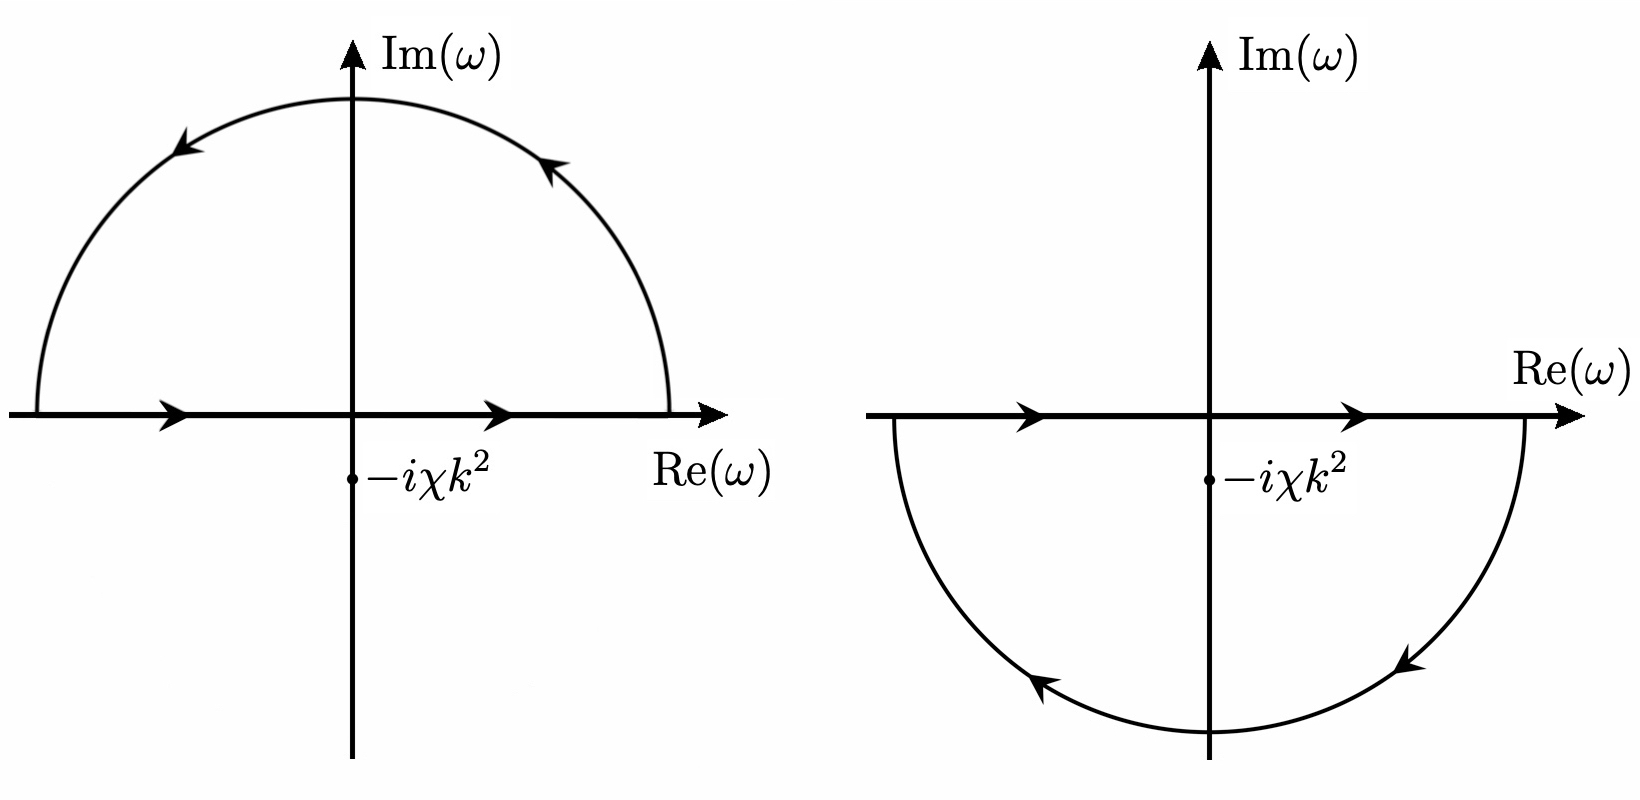
\includegraphics[width=0.9\textwidth]{immagini/complex}
\end{center}
\[
\oint d\omega\frac{e^{-i\omega\tau}}{-i(\omega+i\chi \kk^2)}=:\oint F(\omega) d\omega
\]
\[
e^{-i\omega\tau}=e^{-i(\mathrm{Re}\omega+i\mathrm{Im}\omega)\tau}
\]
Se $\tau<0$ chiudo sopra $\Rightarrow \oint F(\omega) d\omega = 0$

Se $\tau>0$ chiudo sotto $\Rightarrow \oint F(\omega) d\omega \ne 0$

\smallskip

Vogliamo che i contributi dei semicerchi siano nulli quindi:

Per $\tau=t-t'<0$:
\[
F(\omega)d\omega \overset{\omega=\rho e^{i\varphi}}{=}\frac{e^{-i\tau(\rho\cos\varphi+i\rho\sin\varphi)}}{-i(\rho e^{i\varphi}+i\chi \kk^2)}\rho e^{i\varphi}id\varphi=:f(\varphi)d\varphi
\]
Vado a risolvere l'integrale
\[
\left|\int_{0}^{\pi}f(\varphi)d\varphi\right|\leq\int_{0}^{\pi}\left|f(\varphi)\right|d\varphi=
\int_{0}^{\pi}\frac{e^{\tau\rho\sin\varphi}\rho d\varphi}{\left|\rho e^{i\varphi}+i\chi \kk^2\right|}=
\]
\[
=\int_{0}^{\pi}\frac{e^{\tau\rho\sin\varphi}\rho d\varphi}{\sqrt{\left(\rho\cos\varphi\right)^2+\left(\rho\sin\varphi+\chi \kk ^2\right)^2}}
=\int_{0}^{\pi}\frac{e^{\tau\rho\sin\varphi}\rho d\varphi}{\sqrt{\rho^2+2\rho\sin\varphi\chi \kk ^2+\chi^2 \kk^4}}
\]
Posso minorare il denominatore con $\rho$ e ottengo:
\[
\left|\int_{0}^{\pi}f(\varphi)d\varphi\right|
\leq\int_{0}^{\pi}\frac{e^{\tau\rho\sin\varphi}\rho d\varphi}{\rho}=2\int_{0}^\frac{\pi}{2}e^{\tau\rho\sin\varphi} d\varphi
\]
In $[0,\frac{\pi}{2}]$ ho che: $\sin\varphi\geq\frac{2\varphi}{\pi}$

%inserisci immagine

Per $\tau<0$: $\tau\rho\sin\varphi \leq \tau\rho\frac{2\varphi}{\pi}$
\[
\Rightarrow 2\int_{0}^\frac{\pi}{2}e^{\tau\rho\sin\varphi}d\varphi \leq 2\int_{0}^\frac{\pi}{2}e^{\tau\rho\frac{2\varphi}{\pi}}=
2\left[\frac{\pi}{2\tau\rho}e^{\tau\rho\frac{2\varphi}{\pi}}\right]_{0}^{\frac{\pi}{2}}=
\frac{\pi}{\tau\rho}(e^{\tau\rho}-1)\xrightarrow[\rho \rightarrow \infty]{} 0
\]
\[
\Rightarrow G(\z,\tau)=0
\]

Analogamente si dimostra che anche il contributo del cammino sotto l'integrale tende a 0 per $\rho\to\infty$.

\thinspace

Restano da calcolare i residui:
\[
\operatorname{Res}F(\omega)=\lim_{\omega \to -i\chi \kk^2} F(\omega) (\omega + i\chi \kk^2)=ie^{-\tau\chi \kk ^2}
\]
Per $\tau>0$ chiudo l'integrale sotto. Il valore dell'integrale sull'asse reale \`e la differenza tra l'integrale sul cammino chiuso e quello sul solo semicerchio sotto.
%inserisco i simboli di integrali di cammino descritti sopra
\[
\int_{-\infty}^{+\infty}d\omega\, F(\omega)=-2\pi i \operatorname{Res}F(\omega)=2\pi e^{-\tau\chi\kk ^2}
\]
\[
\Rightarrow G(\z,\tau)=\frac{1}{(2\pi)^n}\int d^n\kk\, e^{i\kk\cdot \z-\tau\chi\kk ^2} =\frac{1}{(2\pi)^n}\exp\left(\frac{-\z^2}{4\tau\chi}\right) \int d^n\kk \, e^{-\tau\chi\left(\kk -\frac{i\z}{2\tau\chi}\right)^2}=
\]
\[
=\frac{1}{(2\pi)^n}\exp\left(-\frac{\z^2}{4\tau\chi}\right)\left( \frac{\pi}{\chi\tau} \right)^\frac{n}{2}
\]
\begin{equation}
G(\z,\tau)=\frac{1}{(4\pi\tau\chi)^\frac{n}{2}}\exp\left(-\frac{\z^2}{4\chi\tau}\right), \quad \tau>0
\end{equation}
\`E il nucleo del calore!
\begin{equation}
G(\z,\tau)=0,\quad \tau<0
\end{equation}

Soluzione particolare dell'equazione del calore con sorgente:
\[
T_\text{p}(\x,t)\overset{\eqref{2.17}}{=}\int d^n\x'\int_{-\infty}^{t}dt'\,G(\x-\x',t-t')S(\x',t')
\]

Soluzione generale dell'equazione omogenea:
\[
T_\text{om}(\x,t)\overset{\eqref{2.11}}{=}\int d^n\x'\,G(\x-\x',t)T_0(\x')
\]

Soluzione generale dell'equazione non omogenea:
\[
T(\x,t)=T_\text{p}(\x,t)+T_\text{om}(\x,t)
\]

Se $S(\x',t')=0$ per $t'<0$ $\Rightarrow T_p(\x,0)=0$ e quindi abbiamo che $T(\x,0)=T_\text{om}(\x,0)=T_0(\x)$.

\paragraph{Equazione del calore con bordo}

Considera il problema di Dirichlet in un dominio connesso (o su una variet\`a con bordo) $U$.
\[
\begin{cases}
\Delta \phi + \lambda\phi =0 & \text{in } U \\
\phi=0 & \text{su }\partial U
\end{cases}
\]
$\lambda_n$ : autovalori del problema di Dirichlet per l'operatore $\Delta$, $\phi_n$: autofunzioni di $\Delta$

\begin{equation}
G(t,\x,\y)=\sum_{n}e^{-\lambda_n\chi t}\phi_n(\x)\phi_n(\y )
\label{2.20}
\end{equation}

\begin{equation}
T(\x,t)=\int d^d\y\, G(t,\x,\y)T_0(\y )=\int d^d \y \sum_{n}e^{-\lambda_n\chi t}\phi_n(\x)\phi_n(\y )T_0(\y )
\label{2.21}
\end{equation}

La \eqref{2.20} \`e un esempio di una funzione di Green che non dipende solo la $\x-\y $, ma da $\x$ e $\y $ separatamente. 
Ci\`o \`e dovuto alla rottura dell'invarianza per traslazioni a causa della presenza del bordo $\partial U$.

\medskip

Check: 
\[
T(\x,0)\overset{\eqref{2.21}}{=}\int d^d \y \sum_{n}\phi_n(\x)\phi_n(\y )T_0(\y )=\int d^d\y\, \delta(\x-\y )T_0(\y )=T_0(\x) \quad \checkmark
\]
\[
T(\x,t)\Big|_{\x\in\partial U}=\int d^d\y \sum_n e^{-\lambda_n \chi t} \phi_n(\x)\Big|_{\x\in\partial U}\phi_n(\y )T_0(\y )=0 \quad \checkmark
\]
\[
\frac{\partial}{\partial t}T(\x,t)=\int d^d\y \sum_n (-\lambda_n \chi)e^{-\lambda_n\chi t} \phi_n(\x)\phi_n(\y )T_0(\y )
\]
\[
\chi\Delta_{\x}T(\x,t)=\int d^d \y  \sum_n e^{-\lambda_n \chi t}\chi \underbrace{\Delta_{\x}\phi_n(\x)}_{-\lambda_n \phi_n(\n)} \phi_n(\y )T_0(\y )=\frac{\partial}{\partial t}T(\x,t) \quad \checkmark
\]

\medskip

\underline{Esempio}: $U=[0,L]$

Risolvere:
\[
\partial_t T=\chi\partial_{x}^2T, \qquad x\in[0,L], \qquad t\geq0
\]
Con condizioni al contorno: $T(0,t)=T(L,t)=0$, $T(x,0)=T_0(x)$

\[
\partial^{2}_{x}\phi(x)=-\lambda\phi(x) 
\]
\[
\Rightarrow \phi_n(x)=\phi_0\sin{\left(\sqrt{\lambda_n}\, x\right)},\quad \lambda_n=\frac{n^2\pi^2}{L^2}, \quad n=0,1,2,\dots
\]
\[
\int_0^L dx\, \phi^2_n(x)=1\Rightarrow\phi_0=\sqrt{\frac{2}{L}}
\]
\begin{equation}
\eqref{2.20}\Rightarrow G(t,x,y)=\frac{2}{L}\sum_{n=1}^{\infty}e^{-\frac{n^2\pi^2}{L^2}\chi t}\sin{\left(\frac{n\pi}{L}x\right)}\sin{\left(\frac{n\pi}{L}y\right)}
\label{2.22}
\end{equation}
\begin{equation}
\eqref{2.21}\Rightarrow T(x,t)=\frac{2}{L}\int_0^L dy\sum_{n=1}^{\infty}e^{-\frac{n^2\pi^2}{L^2}\chi t} \sin{\left(\frac{n\pi}{L}x\right)}\sin{\left(\frac{n\pi}{L}y\right)} T_0(y)
\label{2.23}
\end{equation}

Sviluppo $T_0(y)$ in serie di Fourier: 
\begin{equation}
T_0(y)=\sum_{n=1}^{\infty}b_n\sin{\left(\frac{n\pi}{L}y\right)}
\label{2.24}
\end{equation}
con 
\begin{equation}
b_n=\frac{2}{L}\int_0^LT_0(y)\sin{\left(\frac{n\pi}{L}y\right)} dy
\label{2.25}
\end{equation}

Usando la \eqref{2.25}, posso riscrivere la \eqref{2.23} come:
\begin{equation}
T(x,t)=\sum_{n=1}^{\infty}e^{-\frac{n^2\pi^2}{L^2}\chi t}b_n\sin{\left(\frac{n\pi}{L}x\right)}
\end{equation}

N.B.: 
\begin{itemize}
\item La \eqref{2.20} vale anche per variet\`a compatte senza bordo (p.e. $S^2$).
\item La \eqref{2.22} \`e un esempio di funzione di Green che dipende da $x$ e $y$ separatamente. Il motivo \`e la rottura dell'invarianza per traslazioni a causa della presenza del bordo.
\end{itemize}

\medskip

\underline{Esercizi}:

\begin{enumerate}[label=(\roman*)]

\item Risolvere: $\partial_t T=\chi\Delta T$ nel cubo

$x\in[0,L]$, $y\in[0,L]$, $z\in[0,L]$, $t\geq 0$

Con le condizioni: $T(\x,t)=0$, $T(\x,0)=T_0(\x)$

$x=0,L \quad y=0,L \quad z=0,L $

\item Le \eqref{2.20}, \eqref{2.21} valgono anche per il problema di Neumann 
\[
\begin{cases}
\Delta\phi + \lambda\phi =0 & \text{in }U\\
\vect{n}\cdot \nabla\phi=0 & \text{su }\partial U
\end{cases}
\]
dove $\vect{n}$ \`e il versore normale al bordo. Perch\'e? 

(p.e. verificare che $\vect{n}\cdot\nabla T\big|_{\x\in \partial U}=0$)

Risolvere l'equazione del calore nel cubo con pareti isolate (cio\`e nessun flusso termico attraverso le pareti, vedi equazione \eqref{2.1})

$T(\x,0)=T_0(\x)$

$\partial_x T=0 \quad x=0,L$

$\partial_y T=0 \quad y=0,L$

$\partial_z T=0 \quad z=0,L$

(modello per stanza perfettamente isolata)

\item Risolvere l'equazione del calore sulla 2-sfera. 
 
Suggerimento: scrivere il laplaciano in coordinate sferiche
\begin{equation}
\Delta =\frac{1}{r^2}\partial_r(r^2\partial_r)+\frac{1}{r^2\sin\theta}\partial_{\theta} (\sin\theta\partial_{\theta})+\frac{1}{r^2\sin^2\theta}\partial^2\varphi
\end{equation}

Porre $r=cost$ e usare:
\begin{equation}
\frac{1}{\sin\theta}\partial_{\theta}(\sin\theta\partial_\theta Y^m_l)+\frac{1}{\sin^2\theta}\partial^2_{\varphi}Y_l^m=-\lambda Y_l^m
\end{equation}
con $\lambda=l(l+1)$ e $Y_l^m$ armoniche sferiche. 

Sostituire le \eqref{2.24}, \eqref{2.25} col corrispondente sviluppo in armoniche sferiche.
\end{enumerate}

\medskip

\emph{Parentesi}: Soluzione di
\[
\Delta_{\x}G(\x-\y )=-\delta(\x-\y )
\]
in $d$ dimensioni.

Consideriamo un problema un po' pi\`u generale:
\begin{equation}
(\Delta_{\x}-m^2)G(\x-\y )=-\delta(\x-\y )
\end{equation}
$\rightarrow$ $G$ \`e il nucleo dell'equazione di \emph{Helmholtz} 
\begin{equation}
(\Delta_{\x}-m^2)f=-S
\end{equation}
(soluzione: $f(\x)=\int d^d\x'G(\x-\x')S(\x')$)

$G$ \`e il propagatore per un campo scalare in $d$ dimensioni euclidee ($\rightarrow$ teoria quantistica dei campi). 

Uso la trasformata di Fourier per riportarmi ad un'equazione algebrica:
\[
G(\x-\y )=\frac{1}{(2\pi)^d}\int d^d \kk\, e^{i\kk \cdot(\x-\y )}\tilde{G}(\kk )
\]
\[
\delta(\x-\y )=\frac{1}{(2\pi)^d}\int d^d \kk\, e^{i\kk \cdot(\x-\y )}
\]
\[
\Rightarrow (-k^2-m^2)\tilde{G}(\kk )=-1\Rightarrow \tilde{G}(\kk )=\frac{1}{\kk ^2+m^2}
\]
\begin{equation}
\Rightarrow G(\z)=\frac{1}{(2\pi)^d}\int d^d \kk  \frac{e^{i\kk\cdot \z}}{\kk ^2+m^2}
\end{equation}
Uso:
\begin{equation}
\frac{1}{\kk ^2+m^2}=\int_0^{\infty}\exp\left( -\tau(\kk ^2+m^2)\right)d\tau
\end{equation}
\[
\Rightarrow G(\z)=\frac{1}{(2\pi)^d}\int_0^{\infty}d\tau\, e^{-\tau m^2}\int d^d \kk \, e^{i\kk\cdot \z-\tau\kk ^2}
\]
Mi riconduco all'integrale gaussiano con:
\[
i\kk\cdot\z-\tau\kk^2=-\tau\left(\kk-\frac{i\z}{2\tau}\right)^2-\frac{\z^2}{4\tau} \qquad \kp:=\kk-\frac{i\z}{2\tau}
\]
\[
\Rightarrow G(\z)=\frac{1}{(2\pi)^d}\int_0^{\infty}d\tau \, e^{-\tau m^2-\frac{\z^2}{4\tau}} \int d^d\kp \, e^{-\tau\kp^2}
\]
\[
\int d^d\kp \, e^{-\tau\kp^2}=\left(\frac{\pi}{\tau}\right)^\frac{d}{2} \quad (\tau>0)
\]
\[
G(\z)=\frac{1}{(4\pi)^\frac{d}{2}} \int_{0}^{\infty} d\tau\, \tau^{-\frac{d}{2}}e^{-\tau m^2 - \frac{\z^2}{4\tau}}
\]
Cambio di variabile:
\[
\tau:=\frac{|\z|}{2m}e^t, \quad d\tau=\frac{|\z|}{2m}e^t dt, \quad \tau^{-\frac{d}{2}}=\left(\frac{|\z|}{2m}\right)^{-\frac{d}{2}}e^{-\frac{d}{2}t}
\]
\[
-\tau m^2-\frac{\z^2}{4\tau}=-\frac{|\z|}{2 m}e^t m^2-\frac{\z^2}{4}\frac{2m}{|\z|}e^{-t}=-m|\z|\cosh t
\]
\[
\Rightarrow G(\z)=\frac{1}{(4\pi)^\frac{d}{2}} \int_{-\infty}^{+\infty}dt \left(\frac{|\z|}{2m}\right)^{1-\frac{d}{2}}e^{(1-\frac{d}{2})t}e^{-m|\z|\cosh t} 
=\int_{-\infty}^{0}\dots+\int_{0}^{+\infty} \dots
\]
Ho che:
\[
\frac{1}{(4\pi)^\frac{d}{2}} \int_{-\infty}^{0}dt \left(\frac{|\z|}{2m}\right)^{1-\frac{d}{2}}e^{(1-\frac{d}{2})t}e^{-m|\z|\cosh t} = 
\]
\[
\overset{t'=-t}{=}\frac{1}{(4\pi)^\frac{d}{2}} \int_{0}^{+\infty}dt' \left(\frac{|\z|}{2m}\right)^{1-\frac{d}{2}}e^{-(1-\frac{d}{2})t'}e^{-m|\z|\cosh t'}
\]
\[
\overset{t'\rightarrow t}{\Rightarrow} G(\z)=\frac{1}{(4\pi)^\frac{d}{2}}\int_0^{+\infty}dt\left(\frac{|\z|}{2m}\right)^{1-\frac{d}{2}} 2\cosh{ \left[\Big(1-\frac{d}{2}\Big)t\right]}e^{-m|\z|\cosh t}
\]

Definendo la funzione di Bessel modificata del secondo tipo:
\begin{equation}
K_{\nu}(x)=\int_0^{\infty}e^{-x\cosh t}\cosh(\nu t) dt
\end{equation}
\[
\Rightarrow G(\z)=\frac{1}{(4\pi)^\frac{d}{2}}\left(\frac{|\z|}{2m}\right)^{1-\frac{d}{2}} 2 K_{1-\frac{d}{2}}\big(m|\z|\big)
\]
\[
\operatorname{Re}(x)>0 \Rightarrow K_{-\nu}(x)=K_{\nu}(x)
\]
\begin{equation}
\Rightarrow G(\z)=\frac{1}{(2\pi)^\frac{d}{2}}m^{d-2}\big(|\z|m\big)^{1-\frac{d}{2}} K_{\frac{d}{2}-1}\big(m|\z|\big)
\label{2.34}
\end{equation}

Per $m\to 0$ posso usare:
\begin{equation}
K_{\nu}(x)\underset{x \to 0}{\sim}
\begin{cases}
-\gamma-\ln \frac{x}{2} & \nu=0 \\
\frac{\Gamma(\nu)}{2}\left(\frac{2}{x}\right)^{\nu} & \nu >0
\end{cases}
\label{2.35}
\end{equation}
dove $\gamma=\lim_{n\to\infty}\left(\sum_{k=1}^{n}\frac{1}{k}-\ln n\right)\approx 0,577$ (costante di Eulero-Mascheroni)

$\Gamma(\nu)$: funzione gamma di Eulero, estende il concetto di fattoriale ai numeri complessi, nel senso che per ogni numero intero non negativo $n$ si ha $\Gamma (n)=(n-1)!$
\begin{equation}
\Gamma(z)=\int_0^{\infty}t^{z-1}e^{-t}dt,\quad \operatorname{Re}(z)>0
\end{equation}

\underline{Esercizio}: Integrando per parti, dimostrare che:
\begin{equation}
\Gamma(z+1)=z\Gamma(z)
\end{equation}
\[
\Rightarrow \Gamma(z)=\frac{\Gamma(z+1)}{z}
\]
Usando questa definizione la $\Gamma$ pu\`o essere estesa al piano $\operatorname{Re}(z)<0$

$\Rightarrow$ Per $d>2$ e $m\to 0$, la \eqref{2.34} diventa:
\begin{equation}
G(\z)\rightarrow \frac{1}{(2\pi)^\frac{d}{2}} m^{\frac{d}{2}-1}|\z|^{1-\frac{d}{2}}\frac{\Gamma(\frac{d}{2}-1)}{2}\left(\frac{2}{m|\z|}\right)^{\frac{d}{2}-1}=\frac{\Gamma(\frac{d}{2}-1)}{4\pi^\frac{d}{2}|\z|^{d-2}}
\end{equation}
che corrisponde al potenziale di una carica puntiforme in $d$ dimensioni.

\medskip

Caso $d=3$:
\begin{equation}
\Gamma\left(\frac{1}{2}\right)=\sqrt{\pi} \Rightarrow G(\z)=\frac{1}{4\pi|\z|}
\tag{$\theequation^\prime$}
\label{2.38'}
\end{equation}

Caso limite $d=2$:
\begin{equation}
\eqref{2.34}\Rightarrow G(\z)=\frac{1}{2\pi}K_0\big(m|\z|\big)\underset{m\to 0}{\overset{\eqref{2.35}}{\rightarrow}} \frac{1}{2\pi}\left(-\gamma -\ln \frac{m|\z|}{2}\right)
\end{equation}
%\[=\frac{1}{2\pi}(-\gamma -\ln m + \ln 2 - ln|\z|)\]
\`E chiaro che la $G$ \`e definita a meno di una costante additiva nel caso $m\to 0$
\begin{equation}
\Rightarrow G(\z)=-\frac{\ln |\z|}{2\pi}
\end{equation}

\medskip

Check:
\[
\Delta_{\x}G(\x)=-\delta(\x)
\]

A causa dell'invarianza per rotazioni, $G$ dipende solo da $|\x|$.

Coordinate polari:
\[
\Delta =\frac{\partial^2}{\partial r^2}+\frac{1}{r}\frac{\partial}{\partial r}+\frac{1}{r^2}\frac{\partial ^2}{\partial \varphi^2}
\]
Considero $r\neq 0$ (e uso $\frac{\partial G}{\partial \varphi}=0$)
\[
\Delta G = \left(\frac{\partial^2}{\partial r^2}+\frac{1}{r}\frac{\partial}{\partial r}\right)\frac{-\ln r}{2\pi}=\frac{1}{2\pi}\left(\frac{1}{r^2} - \frac{1}{r^2}\right)=0\qquad \checkmark
\]

Integro $\Delta G$ su un disco $D$ centrato in 0, con raggio $\varepsilon$:
\begin{center}
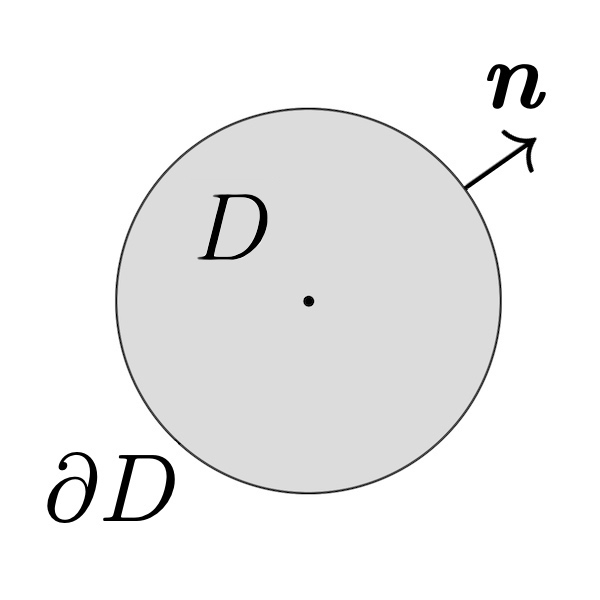
\includegraphics[width=0.2\textwidth]{immagini/disco}
\end{center}
\[
\int_D \Delta G \, d^2\x=\int_D \nabla\cdot(\nabla G) \, d^2\x \overset{\text{Gauss}}{=}\int_{\partial D} \vect{n} \cdot \nabla G \, ds
\]
con $\vect{n}=\hat{\vect{e}}_r$ (versore normale), $ds=r\,d\varphi$ (elemento di linea sul cerchio)
\[
\int_{\partial D}\vect{n}\cdot \nabla G \, ds=\int_{0}^{2\pi}\left(\frac{\partial}{\partial r}G\right)r \, d\varphi=\int_0^{2\pi}-\frac{1}{2\pi r}r \, d\varphi =-1 =-\int_D \delta(\x)\, d^2\x \quad \checkmark
\]
Il laplaciano di $G$ \`e quindi diverso da zero nell'origine.

\subsection{Flusso di calore in un cilindro infinito}

\begin{minipage}{0.3\textwidth}
\centering
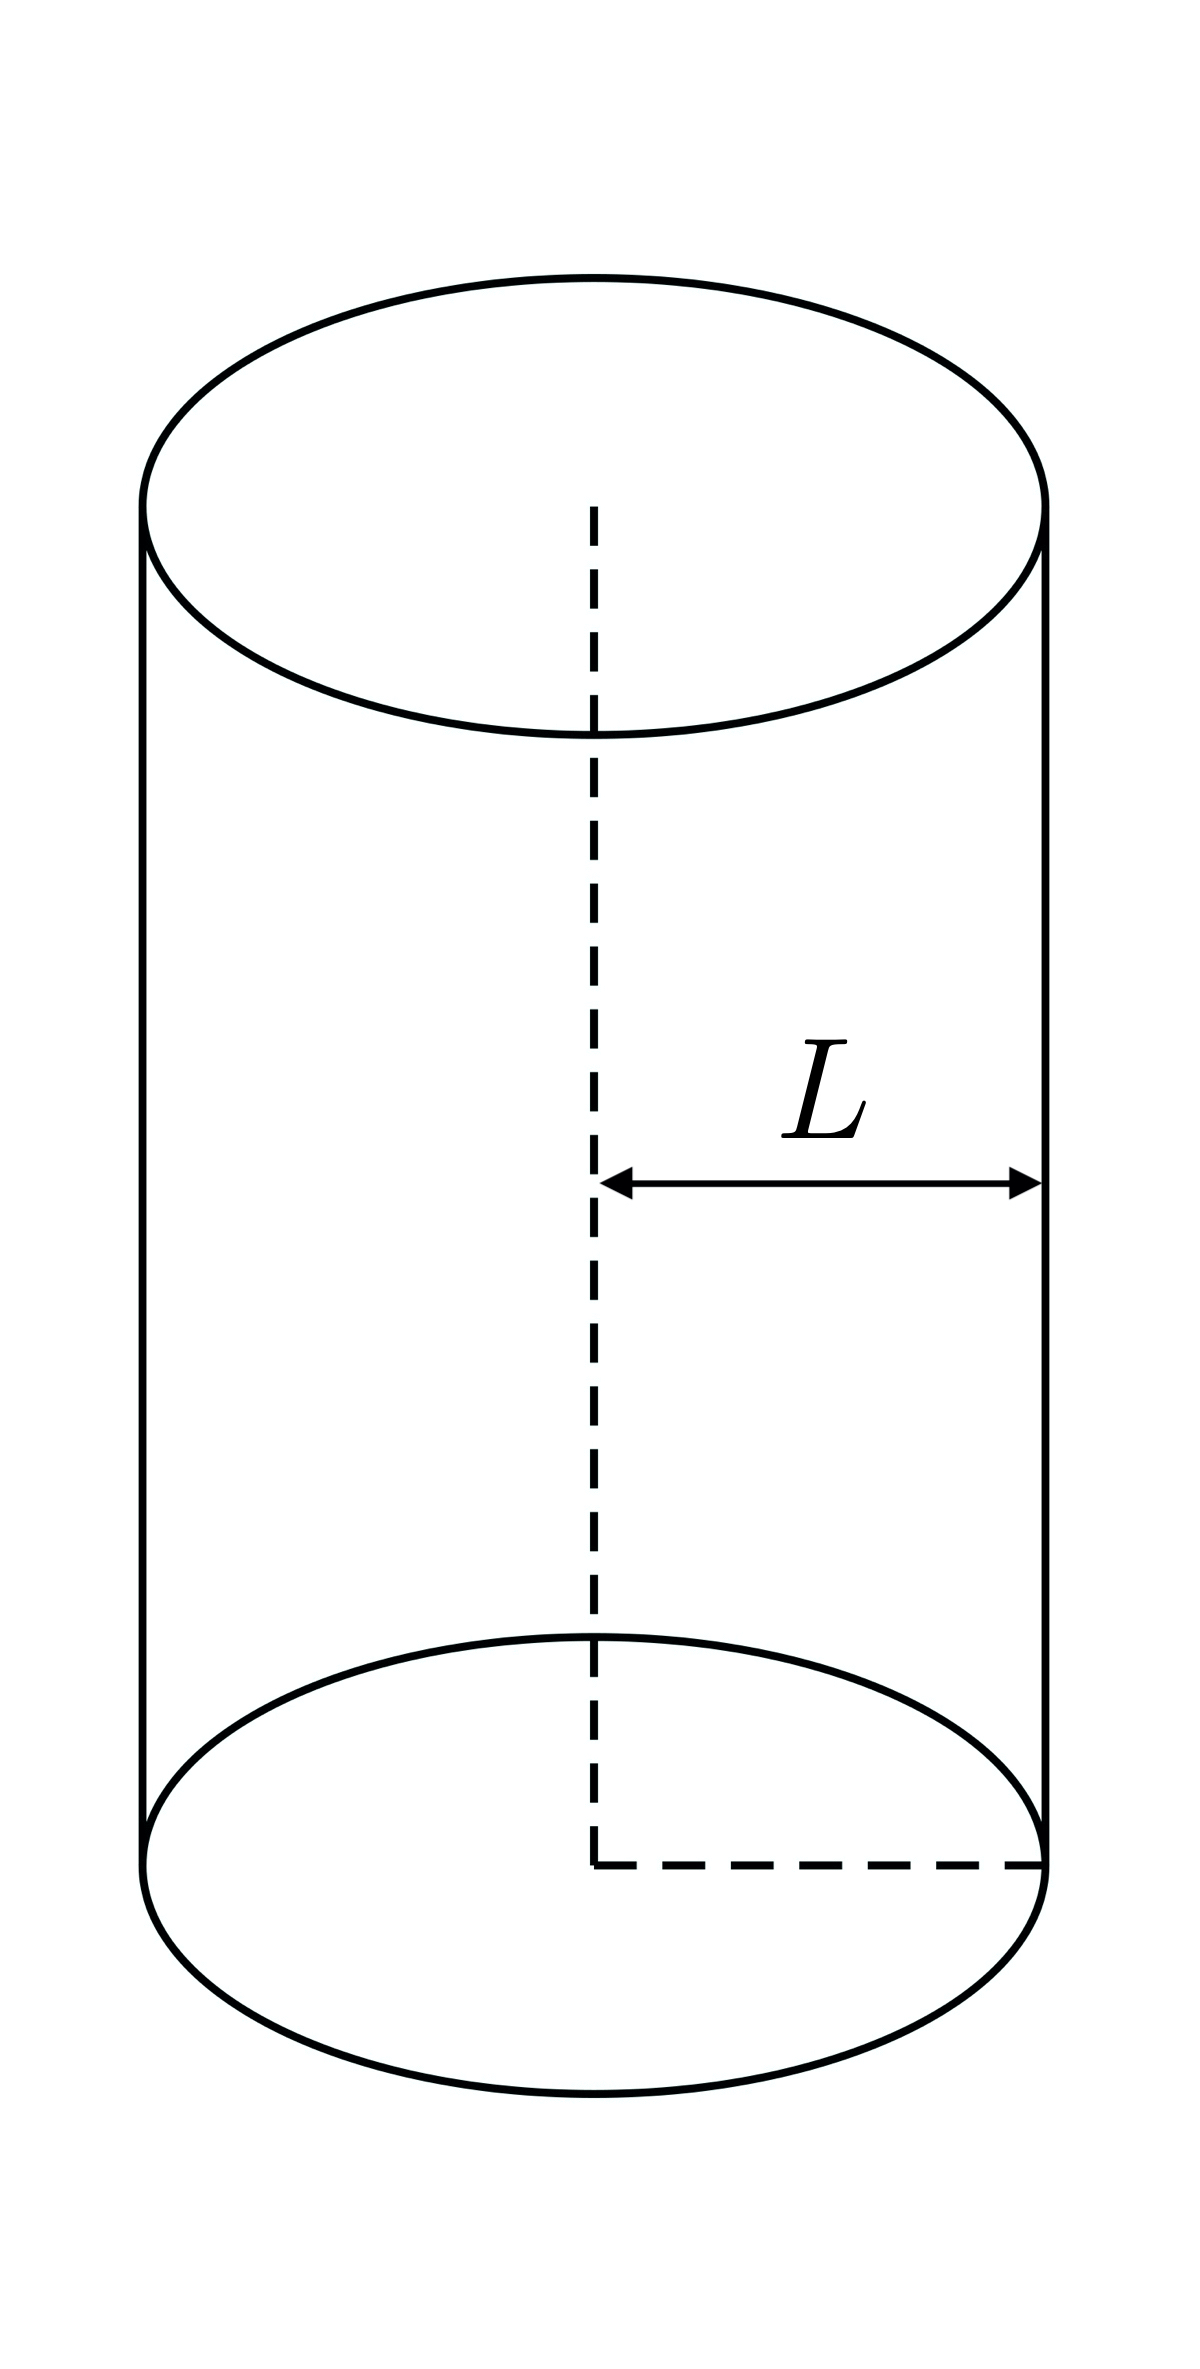
\includegraphics[width=0.6\textwidth]{immagini/simm_cil}
\end{minipage}
\begin{minipage}{0.4\textwidth}
\begin{align*}
\frac{\partial}{\partial t}T=&\chi\Delta T \\
T(\x,t)&=0 \quad \text{per $x$ sul bordo}\\
T(\x,0)&=T_0(\x)
\end{align*}
\end{minipage}

Coordinate cilindriche: $r$, $\varphi$, $z$

con
\[
x=r\cos \varphi, \quad y=r\sin \varphi, \quad z=z
\]
\[
\Delta = \frac{\partial ^2}{\partial r^2} +\frac{1}{r}\frac{\partial}{\partial r} +\frac{1}{r^2} \frac{\partial^2}{\partial \varphi ^2} + \frac{\partial ^2}{\partial z^2}
\]
\[
0\leq r \leq L,\quad 0\leq \varphi \leq 2\pi,\quad -\infty <z<\infty.
\]

Separazione delle variabili:
\[
T(r,\varphi,z,t)=\tau(t)R(r)\Phi(\varphi)Z(z)
\]
\[
\Rightarrow \frac{\partial T}{\partial t}=\tau'R\Phi Z
\]
\[
\Delta T=\tau(R'' +\frac{1}{r}R')\Phi Z + \tau R \frac{1}{r^2}\Phi''Z+\tau R \Phi Z'' \overset{!}{=} \frac{1}{\chi}\tau'R\Phi Z 
\]
\[
\Rightarrow \underbrace{ \frac{1}{R}(R'' + \frac{1}{r}R') + \frac{1}{r^2} \frac{\Phi''}{\Phi}}_{C_1-C_2}+\underbrace{\frac{Z''}{Z}}_{C_2}-\underbrace{\frac{1}{\chi}\frac{\tau'}{\tau}}_{C_1}=0
\]
La funzione di $z$ \`e costante $=C_2$, analogamente la funzione di $t$ $=C_2$ e di conseguenza la parte rimanente funzione di $r,\varphi$ \`e costante $=C_1-C_2$.

Questo \`e possibile solo se tutte e tre le funzioni sono costanti. L'equazione differenziale alle derivate parziali si \`e separata in un insieme di equazioni differenziali ordinarie.

Risolvo:
\[
\tau'=\chi\tau C_1 \Rightarrow \tau=\tau_0 e^{\chi C_1 t} 
\]
\[
Z''=C_2Z \Rightarrow Z=Z_0e^{\sqrt{C_2}z}+Z_1e^{-\sqrt{C_2}z}
\]
\[
r^2\frac{1}{R}(R''+\frac{1}{r}R')+\frac{\Phi''}{\Phi}=(C_1-C_2)r^2 
\]
Pongo:
\[
\frac{\Phi''}{\Phi}=-\lambda^2=cost
\]
e ottengo:
\[
r^2\frac{1}{R}(R''+\frac{1}{r}R')+ (C_2-C_1)r^2=\lambda^2
\]
Risolvo l'equazione per $\Phi$:
\[
\Rightarrow \Phi=\Phi_0 \cos{(\lambda\varphi)} + \Phi_1\sin{(\lambda\varphi)}\overset{!}{=}
\Phi_0\cos{\big(\lambda(\varphi+2\pi)\big)}+\Phi_1\sin{\big(\lambda(\varphi+2\pi)\big)}=
\]
\[
=\Phi_0\big( \cos{(\lambda\varphi)} \cos{( 2\pi\lambda)} - \sin{(\lambda\varphi)} \sin{( 2\pi\lambda)} \big)+
\Phi_1\big( \sin{(\lambda\varphi)} \cos{( 2\pi\lambda)} + \cos{(\lambda\varphi)} \sin{( 2\pi\lambda)} \big)
\]
\[
\Rightarrow \left\{\begin{aligned}
\Phi_0\cos{(2\pi\lambda)} + \Phi_1 \sin{(2\pi\lambda)}=&\Phi_0\\
-\Phi_0\sin{(2\pi\lambda)} + \Phi_1 \cos{(2\pi\lambda)}=&\Phi_1
\end{aligned}\right.
\]
\[
\Rightarrow
\left(\begin{matrix}
\cos( 2\pi\lambda) -1 & \sin( 2\pi\lambda) \\
-\sin( 2\pi\lambda) & \cos( 2\pi\lambda) -1
\end{matrix}\right)
\left(\begin{matrix}
\Phi_0\\
\Phi_1
\end{matrix}\right)
=0
\]
Ho soluzione non banale solo per determinante nullo

$\Rightarrow \cos (2\pi\lambda)=1, \quad \sin (2\pi\lambda)=0$  

$\Rightarrow \lambda=m, \quad m \in \mathbb{Z}$. 

Basta prendere $m\in \mathbb{N}_0$, per cui le funzioni $\Phi$ formano un sistema completo.

$\rightarrow $ L'equazione radiale diventa:
\[
r^2 R'' + r R' + \big((C_2-C_1)r^2-m^2\big)R=0
\]
Supponiamo (per semplicit\`a) che $T_0(\x)$ dipenda solo da $r,\varphi$ e non da $z$:
\[
T(r,\varphi,z,0)=\tau_0R\Phi Z\overset{!}{=}T_0(r,\varphi)\Rightarrow Z=cost \Rightarrow C_2=0
\]
\[
Z=Z_0e^{\sqrt{C_2}z}+Z_1e^{-\sqrt{C_2}z}
\]
Senza perdere la generalit\`a poniamo $Z=1$

$C_1<0$ altrimenti $T$ diverge per $t\to \infty$ (comportamento non fisico). 
%$\quad(\tau=\tau_0e^{\chi C_1 t})$

Inoltre si pu\`o far vedere che la soluzione dell'equazione radiale (con $C_2=0$) diverge nell'origine (per le nostre condizioni al contorno) se $C_1>0$.

Definisco una nuova variabile radiale: $x:=\sqrt{|C_1|}r$

\begin{equation}
\Rightarrow x^2\frac{d^2 R}{dx^2}+x\frac{dR}{dx}+(x^2-m^2)R=0
\label{2.41}
\end{equation}
\centerline{\emph{Equazione differenziale di Bessel}}

\medskip

Risolviamo cercando una soluzione in serie di potenze.

Ansatz: cerchiamo soluzioni della forma:

\begin{equation}
R(x)=x^\alpha \sum_{n=0}^{\infty} a_nx^n \qquad a_0\neq 0
\end{equation}
\[
R'(x)=\alpha x^{\alpha -1}\sum_n a_nx^n + x^\alpha\sum_n na_nx^{n-1}
\]
\[
R''(x)=\alpha(\alpha-1)x^{\alpha-2}\sum_na_nx^n + 2\alpha x^{\alpha-1}\sum_n n a_n x^{n-1}+x^\alpha\sum_n n(n-1)a_nx^{n-2}
\]
Sostituisco nella \eqref{2.41}:
\[
\alpha(\alpha-1)x^\alpha\sum_n a_n x^n+2\alpha x^\alpha \sum_n n a_n x^n + x^\alpha \sum_n n(n-1)a_n x^n \,+
\]
\[
+\, \alpha x^\alpha\sum_n a_n x^n + x^\alpha \sum_n n a_n x^n + (x^2-m^2)x^\alpha \sum_n a_n x^n=0
\]

Dopo opportune semplificazioni, dividendo quello che rimane per $x^\alpha$, ottengo:
\[
(\alpha^2-m^2)\sum_n a_n x^n + \sum_n a_n x^{n+2} + 2 \alpha \sum_n n a_n x^n + \sum_n n^2 a_n x^n = 0
\]

Studio il prefattore di $x^0$: 
\[
\alpha^2 a_0-m^2a_0=0\Rightarrow \alpha=\pm m
\]
Scarto la soluzione $\alpha=-m$ perch\'e non fisica (divergerebbe sull'asse del cilindro).

Soluzione regolare in $x=0$: $\alpha=m$. 

In tal caso:
\begin{equation}
2m\sum_n n a_n x^n + \sum_n n^2 a_n x^n + \sum_n a_n x^{n+2}=0
\label{2.43}
\end{equation}
Riscrivo l'ultima parte:
\[
\sum_{n=0}^{\infty} a_{n} x^{n+2}\overset{n'=n+2}{=}\sum_{n'=2}^{\infty} a_{n'-2} x^{n'}=\sum_{n=2}^{\infty} a_{n-2} x^{n}
\]

Studio il prefattore di $x^1$:
\[
2ma_1+a_1=0 \Rightarrow a_1=0 
\]
$\Rightarrow$ la \eqref{2.43} diventa:
\[
\sum_{n=2}^{\infty}x^n\big(a_n(2mn+n^2)+a_{n-2}\big)=0 
\]
\begin{equation}
\Rightarrow a_n = - \frac{a_{n-2}}{2mn+n^2}
\end{equation}
$\rightarrow$ relazione di ricorrenza

Scegliendo $a_0=\frac{2^{-m}}{m!}$ per motivi di normalizzazione, si ottiene la soluzione:
\begin{equation}
J_m(x)=\sum_{k=0}^{\infty}\frac{(-1)^k\left(\frac{x}{2}\right)^{m+2k}}{k!(m+k)!}
\end{equation}
dove per $m$ non interi si definisce $m!=\Gamma(m+1)$ in termini della funzione gamma.

$J_m:$ \emph{funzione di Bessel del primo tipo}

\begin{center}
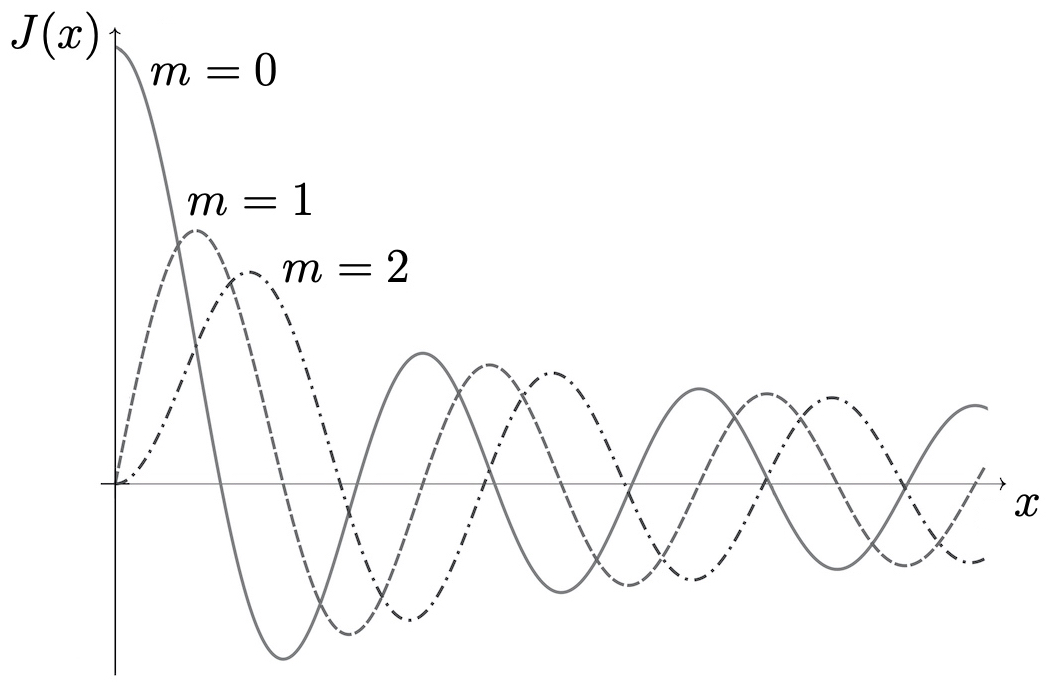
\includegraphics[width=0.65\textwidth]{immagini/bessel}
\end{center}
\[
\Rightarrow R=J_m(\sqrt{|C_1|}r)
\]
La costante di integrazione pu\`o essere determinata imponendo le condizioni al contorno:
\[
T(r=L,\varphi,z,t)\overset{!}{=}0 \Rightarrow R(r=L)=0
\]
\[
\Rightarrow J_m(\sqrt{|C_1|}L)=0 \Rightarrow \sqrt{|C_1|}L=j_k^{(m)}, \quad k=1,2,\dots
\]
dove $j_k^{(m)}$ sono gli zeri positivi di $J_m(x)$, noti numericamente.
\[
\Rightarrow C_1=-\left(\frac{j_k^{(m)}}{L}\right)^2
\]
\[
\Rightarrow T(r,\varphi,z,t)=\tau_0e^{-\chi \left(j_k^{(m)}/L\right)^2 t} J_m\left(j_k^{(m)}\frac{r}{L}\right)\big(\Phi_0\cos(m\varphi) + \Phi_1 \sin( r\varphi)\big)
\]
La costante $\tau_0$ si pu\`o riassorbire in $\Phi_0$ e $\Phi_1$.

La soluzione generale sar\`a una combinazione lineare di queste soluzioni:
\begin{equation}
T(r,\varphi,z,t)=\sum_{m=0}^{\infty}\sum_{k=1}^\infty e^{-\chi \left( j_k^{(m)} /L \right)^2t} J_m\left(j_k^{(m)}\frac{r}{L}\right) \big(C_{km}\cos (m\varphi) + S_{km}\sin (m\varphi)\big)
\end{equation}

\begin{equation}
T(r,\varphi,z,0)=\sum_{m=0}^{\infty}\sum_{k=1}^\infty \underbrace{J_m\left(j_k^{(m)}\frac{r}{L}\right) \big(C_{km}\cos (m\varphi) + S_{km}\sin (m\varphi)\big)}_\text{sistema completo di funzioni nel cilindro}
\overset{!}{=}T_0(r, \varphi)
\label{2.47}
\end{equation}

$\rightarrow$ qualsiasi funzione $T_0(r,\varphi)$ con $T_0(L,\varphi)=0$ possiede uno sviluppo di questo tipo.

Le costanti $C_{km}$ e $S_{km}$ devono essere scelte tali che la \eqref{2.47} sia soddisfatta.

\section{Problemi non omogenei}

Spesso la separazione delle variabili riduce delle equazioni differenziali alle derivate parziali a delle equazioni differenziali ordinarie, come per esempio:
\begin{equation}
a(x)u''(x) + b(x)u'(x)+c(x)u(x)=F(x) \qquad \alpha<x<\beta
\label{2.48}
\end{equation}

Ipotesi: $a(x)$ continuamente differenziabile; $b(x)$, $c(x)$ continue. 

Moltiplico la \eqref{2.48} con 
\[
\frac{1}{a(x)}\exp\left(\int_\alpha^x\frac{b(\xi)}{a(\xi)}d\xi\right)
\]
e definisco
\[
p(x):= \exp\left(\int_\alpha^x \frac{b(\xi)}{a(\xi)}d\xi\right)
\]
\[
q(x):=\frac{c(x)}{a(x)}p(x),\quad f(x):=\frac{F(x)}{a(x)}p(x)
\]
Posso scrivere la \emph{forma autoaggiunta} della \eqref{2.48}:
\begin{equation}
\frac{d}{dx}\left(p\frac{du}{dx}\right) + qu = f(x)
\end{equation}

\medskip

Digressione:
\[
\underbrace{p\frac{d}{dx}}_{:=\frac{d}{dy}} \left( p\frac{d}{dx}u\right)+\underbrace{pq}_{:=\omega^2}u=\underbrace{pf}_{:=\tilde{f}}
\]
 \[
dy=\frac{dx}{p(x)} \Rightarrow y=\int \frac{dx}{p(x)} 
\]
\[
\Rightarrow \frac{d^2u}{dy^2}+\omega^2 u=\tilde{f} \qquad \omega=\omega(y)
\]
\`E un'equazione di oscillatore forzato con frequenza che dipende dal tempo.
Viene chiamato \emph{oscillatore di Ermakoff}, e trova applicazioni in Cosmologia (equazione di Mukhanov-Sasaki) per quanto riguarda la teoria dell'inflazione.

\medskip

Equazione omogenea: 
\begin{equation}
\frac{d}{dx}\left(p\frac{dv}{dx}\right)+qv=0
\label{2.50}
\end{equation}
Possiede 2 soluzioni ($2^o$ ordine) $v_1, v_2$ linearmente indipendenti.
\[
\rightarrow \text{Wronskiano} \quad
\left| \begin{matrix}
v_1(x) & v_2(x)\\
v_1'(x) & v_2'(x)
\end{matrix}
\right| \neq 0
\]
$\rightarrow$ Soluzione generale:
\[
v(x)=c_1v_1(x) + c_2v_2(x), \quad c_1, c_2 \text{ costanti}
\]

Considera la funzione:
\begin{equation}
w(x)=v_1(x)\int_\alpha^x v_2(\xi)f(\xi)d\xi - v_2(x)\int_\alpha^x v_1(\xi)f(\xi)d\xi
\end{equation}
\centerline{(\emph{Variazione delle costanti})}

\[
\Rightarrow w'(x)=v_1'(x)\int_\alpha^x v_2(\xi)f(\xi)d\xi - v_2'(x)\int_\alpha^x v_1(\xi)f(\xi)d\xi +v_1(x)v_2(x)f(x)-v_2(x)v_1(x)f(x) = 
\]
\[
= v_1'(x)\int_\alpha^x v_2(\xi)f(\xi)d\xi - v_2'(x)\int_\alpha^x v_1(\xi)f(\xi)d\xi 
\]
\[
\Rightarrow\frac{d}{dx}\left(p(x)\frac{dw}{dx}\right)=\underbrace{\frac{d}{dx}\big(p(x)v_1'(x)\big)}_{-qv_1} \int_\alpha^x v_2(\xi)f(\xi)d\xi - \underbrace{\frac{d}{dx}\big(p(x)v_2'(x)\big)}_{-qv_2} \int_\alpha^x v_1(\xi)f(\xi)d\xi \,+
\]
\[
+\, p(x)v_1'(x)v_2(x)f(x)-p(x)v_2'(x)v_1(x)f(x)=-qw +p (v_1' v_2 - v_2' v_1) f
\]

Inoltre:
\[
\frac{d}{dx}\big\{p(x)\big(\underbrace{v_1'(x)v_2(x)-v_2'(x)v_1(x)}_{\text{Wronskiano} \neq0}\big)\big\}=
\]
\[
=\underbrace{\frac{d}{dx}\big(p v_1'\big)}_{-qv_1} v_2- \underbrace{\frac{d}{dx}\big(pv_2'\big)}_{-qv_2} v_1 + pv_1'v_2' - p v_2'v_1'=0
\]
\[
\Rightarrow p(x)\big( v_1'(x)v_2(x)-v_2'(x)v_1(x)\big):=K\quad \text{costante}
\]

Quindi: 
\begin{equation}
\frac{d}{dx}\left(p\frac{dw}{dx}\right)+qw=Kf
\label{2.52}
\end{equation}

Inoltre, se $v_1',v_2'$ sono limitati per $x\to\alpha$: $w(\alpha)=w'(\alpha)=0$

Divido la \eqref{2.52} per $K$ (\`e sempre diversa da 0 poich\'e $p\neq0$ e Wronskiano $\neq0$)

$\Rightarrow$  la funzione $u(x)=\frac{w(x)}{K}$ \`e una soluzione del problema ai valori iniziali
\begin{equation}
\begin{gathered}
\frac{d}{dx}\left(p\frac{du}{dx}\right) + qu=f(x) \qquad x>\alpha \\
u(\alpha)=u'(\alpha)=0
\end{gathered}
\label{2.53}
\end{equation}

\begin{equation}
\Rightarrow u(x)=\int_\alpha^xR(x,\xi)f(\xi)d\xi
\label{2.54}
\end{equation}

con 
\begin{equation}
R(x,\xi):=\frac{v_1(x)v_2(\xi)-v_2(x)v_1(\xi)}{p(x)\big(v_1'(x)v_2(x)-v_2'(x)v_1(x)\big)}
\label{2.55}
\end{equation}
\centerline{\emph{funzione di Green (one-sided)}}

\medskip

Il denominatore della \eqref{2.55} \`e costante $\Rightarrow R(x,\xi)$ soddisfa l'equazione omogenea \eqref{2.50} sia come funzione di $x$ che di $\xi$. 

N.B.:
\[
R(x,\xi)=-R(\xi,x)
\]

Per $\xi$ fissato: $R(x,\xi)$ \`e la soluzione del problema omogeneo ai valori iniziali
\begin{equation}
\begin{gathered}
\frac{d}{dx}\left(p(x)\frac{dR}{dx}\right) + q(x)R(x)=0 \qquad x>\xi \\
R \big|_{x=\xi}=0, \qquad \left.\frac{dR}{dx}\right|_{x=\xi}\overset{\eqref{2.55}}{=}\frac{1}{p(\xi)}
\end{gathered}
\label{2.56}
\end{equation}

\medskip

\underline{Esempio}: \emph{Oscillatore armonico invertito forzato}
\[
\begin{gathered}
u'' - u =f(x) \qquad x>0 \\
u(0)=u'(0)=0
\end{gathered}
\]

Soluzione: Per $\xi$ fissato, $R(x,\xi)$ soddisfa:
\[
\begin{cases}
\frac{d^2R}{dx^2}-R=0, \quad x>\xi \\
R|_{x=\xi}=0\\
\left.\frac{dR}{dx}\right|_{x=\xi}=1
\end{cases}
\]
\[
\Rightarrow R= A(\xi)\sinh(x)+B(\xi)\cosh(x)
\]
\[
\begin{cases}
R|_{x=\xi}=A\sinh\xi + B \cosh \xi =0\\
\left.\frac{dR}{dx}\right|_{x=\xi}=A\cosh\xi + B \sinh \xi =1
\end{cases}
\]
\[
\Rightarrow A=\cosh \xi, \quad B=-\sinh \xi
\]
\[
 \Rightarrow R=\sinh(x-\xi)
\]
\[
\eqref{2.54}\Rightarrow u(x)=\int_0^x f(\xi)\sinh(x-\xi)d\xi
\]

Commenti:
\begin{enumerate}[label=(\roman*)]
\item Se $u(\alpha),u'(\alpha)\neq 0$ aggiungi soluzione $c_1v_1(x)+c_2v_2(x)$ dell'equazione omogenea, in modo tale da soddisfare le nuove condizioni iniziali. 

Nell'esempio sopra:
\[
u(x)=\int_0^x f(\xi)\sinh(x-\xi)d\xi + c_1\sinh(x)+ c_2\cosh(x)
\]
soddisfa $u(0)=c_2$, $u'(0)=c_1$
\item \eqref{2.54} $\Rightarrow$ Il valore di $u(x)$ dipende solo da $f(\xi)$ per  $\xi<x$ (causalit\`a). 

$\rightarrow$ Comportamento molto simile a quello delle equazioni differenziali alle derivate parziali di tipo iperbolico.
%riferimento all'indice?
\end{enumerate}

\subsection{Problema ai valori al contorno}

Risolvi
\begin{equation}
\begin{gathered}
\frac{d}{dx}\left(p\frac{du}{dx}\right)+qu=-f(x) \qquad \alpha <x<\beta\\
u(\alpha)=u(\beta)=0 
\end{gathered}
\label{2.57}
\end{equation}

Soluzione generale:
\[
u(x)=-\int_\alpha^x R(x,\xi)f(\xi)d\xi + c_1v_1(x)+c_2v_2(x) 
\]
\begin{equation}
\Rightarrow\begin{cases}
u(\alpha)=c_1v_1(\alpha)+c_2v_2(\alpha)=0\\
u(\beta)=-\int_{\alpha}^\beta R(\beta,\xi)f(\xi)d\xi + c_1v_1(\beta)+c_2v_2(\beta)=0
\end{cases}
\label{2.58}
\end{equation}
Sistema lineare non omogeneo per le variabili $c_1$ e $c_2$.

La \eqref{2.58} ha una soluzione per $c_1,c_2$ se:
\[
D:=v_1(\alpha)v_2(\beta)-v_2(\alpha)v_1(\beta)\neq 0
\]
In tal caso
\[
c_1=-\frac{v_2(\alpha)}{D}\int_\alpha^\beta R(\beta,\xi)f(\xi)d\xi= -\frac{v_2(\alpha)}{D}\int_\alpha^x R(\beta,\xi)f(\xi)d\xi -\frac{v_2(\alpha)}{D}\int_x^\beta  R(\beta,\xi)f(\xi)d\xi
\]
\[
c_2= \frac{v_1(\alpha)}{D}\int_\alpha^\beta  R(\beta,\xi)f(\xi)d\xi= \frac{v_1(\alpha)}{D}\int_\alpha^x R(\beta,\xi)f(\xi)d\xi +\frac{v_1(\alpha)}{D}\int_x^\beta  R(\beta,\xi)f(\xi)d\xi
\]
E quindi la soluzione diventa:
\[
u(x)=-\int_\alpha^x\left[R(x,\xi)+\frac{v_2(\alpha)v_1(x) - v_1(\alpha)v_2(x)}{D}R(\beta,\xi)\right]f(\xi)d\xi\,+
\]
\[
-\int_x^\beta \frac{v_2(\alpha)v_1(x) - v_1(\alpha)v_2(x)}{D} R(\beta,\xi)f(\xi)d\xi
\]
Consideriamo:
\[
R(x,\xi)+\frac{v_2(\alpha)v_1(x)-v_1(\alpha)v_2(x)}{D}R(\beta,\xi)=
\]
\[
\overset{\eqref{2.55}}{=}\frac{v_1(x)v_2(\xi)-v_2(x)v_1(\xi)}{K D}\big(v_1(\alpha)v_2(\beta)-v_2(\alpha)v_1(\beta)\big)\, +
\]
\[
+\, \frac{v_2(\alpha)v_1(x)-v_1(\alpha)v_2(x)}{D} \frac{v_1(\beta)v_2(\xi)-v_2(\beta)v_1(\xi)}{K}=
\]
\[
=\frac{1}{KD}\big(v_1(\alpha)v_2(\xi)-v_2(\alpha)v_1(\xi)\big) \big(v_1(x)v_2(\beta)-v_2(x)v_1(\beta)\big)
\]

Definiamo:
\begin{equation}
G(x,\xi):=
\begin{cases}
\frac{1}{KD}\big(v_1(\xi)v_2(\alpha)-v_2(\xi)v_1(\alpha) \big)\big(v_1(x)v_2(\beta)-v_2(x)v_1(\beta)\big), & \xi\leq x \\
\frac{1}{KD}\big(v_1(x)v_2(\alpha)-v_2(x)v_1(\alpha) \big)\big(v_1(\xi)v_2(\beta)-v_2(\xi)v_1(\beta)\big), & x\leq \xi
\end{cases}
\label{2.59}
\end{equation}
\centerline{\emph{funzione di Green (two-sided)}}

\medskip

$\Rightarrow$ soluzione del problema ai valori al contorno \eqref{2.57}:
\begin{equation}
u(x)=\int_\alpha^\beta G(x,\xi)f(\xi)d\xi
\end{equation}
N.B.: 
\begin{equation}
G(x,\xi)=G(\xi,x)
\end{equation}

Per determinare $G$ notiamo che, per ogni $\xi$ fissato, la $G$ soddisfa il problema ai valori al contorno:
\begin{equation}
\begin{cases}
\frac{d}{dx}\left(p(x)\frac{dG}{dx}\right) + q(x)G = 0 & x\neq \xi \\
G|_{x=\alpha}=G|_{x=\beta}=0 \\
G|_{x=\xi+0}=G|_{x=\xi-0} & \text{($G$ continua in $x=\xi$)} \\
\frac{dG}{dx}\big|_{x=\xi+0}-\frac{dG}{dx}\big|_{x=\xi-0}=-\frac{1}{p(\xi)} & \text{($\frac{dG}{dx}$ discontinua in $x=\xi$)} \\
\end{cases}
\label{2.62}
\end{equation}
(\underline{Dimostrazione}: Usa la \eqref{2.59}. Per ricavare l'ultima equazione bisogna usare anche la definizione di $K$)

\medskip

\underline{Esempio}: 
\[
\begin{gathered}
\big((1+x)^2u'\big)'-u=f(x) \qquad 0\leq x\leq1\\
u(0)=u(1)=0
\end{gathered}
\]
Scriviamo equazione omogenea
\[
\frac{d}{dx}\left((1+x)^2 \frac{dG(x,\xi)}{dx}\right)-G(x,\xi)=0
\]
Prova $G(x,\xi)=c(\xi)(1+x)^\alpha$
\[ \Rightarrow \frac{dG}{dx}=c\alpha(1+x)^{\alpha-1}
\]
\[
\left((1+x)^2 \frac{dG}{dx}\right)'=\big(c\alpha(1+x)^{\alpha+1}\big)'
=c\alpha(\alpha +1)(1+x)^\alpha \overset{!}{=} G = c(1+x)^\alpha
\]
\[
\Rightarrow \alpha^2 + \alpha - 1 =0 \Rightarrow \alpha=\frac{1}{2}(-1\pm \sqrt{5}):=\alpha_\pm
\]
\[
\Rightarrow  G(x,\xi)=
\begin{cases}
c_+(\xi)(1+x)^{\alpha_+} + c_-(\xi)(1+x)^{\alpha_-}, & x<\xi \\
\tilde{c}_+(\xi)(1+x)^{\alpha_+} + \tilde{c}_-(\xi)(1+x)^{\alpha_-}, & x>\xi
\end{cases}
\]
\[
G|_{x=0}=c_+ + c_- \overset{!}{=} 0 \Rightarrow c_- = -c_+
\]
\[
G|_{x=1}=\tilde{c}_+ 2^{\alpha_+} + \tilde{c}_-2^{\alpha_-} \overset{!}{=} 0 \Rightarrow \tilde{c}_- = -\tilde{c}_+2^{\sqrt{5}} 
\]
\[
\Rightarrow G(x,\xi)=
\begin{cases}
c_+(\xi) \big((1+x)^{\alpha_+} - (1+x)^{\alpha_-} \big), & x<\xi \\
\tilde{c}_+(\xi) \big((1+x)^{\alpha_+} - 2^{\sqrt{5}} (1+x)^{\alpha_-} \big), & x>\xi \\
\end{cases}
\]
\[
\overset{!}{=} G(\xi, x)=
\begin{cases}
c_+(x) \big((1+\xi)^{\alpha_+} - (1+\xi)^{\alpha_-} \big), & \xi<x \\
\tilde{c}_+(x) \big((1+\xi)^{\alpha_+} - 2^{\sqrt{5}} (1+\xi)^{\alpha_-} \big), & \xi>x \\
\end{cases}
\]
\[
\Rightarrow \tilde{c}_+(\xi) \big((1+x)^{\alpha_+} - 2^{\sqrt{5}} (1+x)^{\alpha_-} \big) = c_+(x) \big((1+\xi)^{\alpha_+} - (1+\xi)^{\alpha_-} \big)
\]
\[
\frac{(1+x)^{\alpha_+} - 2^{\sqrt{5}} (1+x)^{\alpha_-} }{c_+(x)}=\frac{(1+\xi)^{\alpha_+} - (1+\xi)^{\alpha_-}}{\tilde{c}_+(\xi)}:=\frac{1}{\lambda} \quad\text{costante}
\]
\[
c_+(x)=\lambda \big((1+x)^{\alpha_+} - 2^{\sqrt{5}} (1+x)^{\alpha_-} \big)
\]
\[
\tilde{c}_+(\xi)=\lambda \big((1+\xi)^{\alpha_+} - (1+\xi)^{\alpha_-} \big)
\]
\[
\Rightarrow G(x,\xi)=
\begin{cases}
\lambda \big( (1+\xi)^{\alpha_+}-2^{\sqrt{5}}(1+\xi)^{\alpha_-}\big) \big( (1+x)^{\alpha_+}-(1+x)^{\alpha_-}\big), & x<\xi \\
\lambda \big( (1+\xi)^{\alpha_+}-(1+\xi)^{\alpha_-}\big) \big( (1+x)^{\alpha_+}-2^{\sqrt{5}}(1+x)^{\alpha_-} \big), & x>\xi \\
\end{cases}
\]
$\Rightarrow G|_{x=\xi+0}=G|_{x=\xi-0}$ (continuit\`a)

Ci manca l'ultima condizione sul salto della derivata e questa mi determina $\lambda$:
\[
\left.\frac{dG}{dx}\right|_{x=\xi+0}=\lambda \big( (1+\xi)^{\alpha_+}-(1+\xi)^{\alpha_-}\big) \big(\alpha_+(1+\xi)^{\alpha_+ -1}-2^{\sqrt{5}}\alpha_-(1+\xi)^{\alpha_- -1}\big)
\]
\[
\left.\frac{dG}{dx}\right|_{x=\xi-0}=\lambda \big( (1+\xi)^{\alpha_+}-2^{\sqrt{5}}(1+\xi)^{\alpha_-} \big) \big(\alpha_+(1+\xi)^{\alpha_+ -1}-\alpha_-(1+\xi)^{\alpha_- -1}\big)
\]
\[
\left.\frac{dG}{dx}\right|_{x=\xi+0}-\left.\frac{dG}{dx}\right|_{x=\xi-0}=
\]
\[
=\lambda \Big[ \alpha_+ (1+\xi)^{2\alpha_+ -1}-2^{\sqrt{5}}\alpha_-(1+\xi)^{\alpha_+ + \alpha_- -1} - \alpha_+(1+\xi)^{\alpha_-+\alpha_+-1} + 2^{\sqrt{5}}\alpha_- (1+\xi)^{2\alpha_- -1}\, +
\]
\[
-\, \alpha_+(1+\xi)^{2\alpha_+ -1}+ \alpha_- (1+\xi)^{\alpha_+ + \alpha_- - 1} + 2^{\sqrt{5}}\alpha_+(1+\xi)^{\alpha_- + \alpha_+ -1}-2^{\sqrt{5}}\alpha_-(1+\xi)^{2\alpha_- -1} \Big]=
\]
\[
\overset{!}{=}-\frac{1}{p(\xi)}=-\frac{1}{(1+\xi)^2}
\]
$\alpha_+ + \alpha_- -1=-2$
\[
\Rightarrow \lambda\left[ -2^{\sqrt{5}}\alpha_- - \alpha_+ + \alpha_- + 2^{\sqrt{5}}\alpha_+\right]=-1
\]
$\Rightarrow$ determina $\lambda$

Nota la funzione di Green, tramite convoluzione ottengo la soluzione.

\subsection{Problema ai valori al contorno pi\`u generale}
%sottosezione? e' il problema di dirichlet piu generale
%dirichlet -> ho fissato al contorno solo la funzione
%neumann-> ho fissato al contorno la funzione e la derivata
%robin-> fisso con una combinazione lineare di u e u', in pratica vincolo posizione e velocita' lungo la traiettoria

\begin{equation}
\begin{gathered}
\big(pu'\big)'+qu=-f \qquad \alpha<x<\beta\\
u(\alpha)=a, \quad u(\beta)=b
\end{gathered}
\label{2.63}
\end{equation}

Sappiamo gi\`a una soluzione della non omogenea $\Rightarrow$ bisogna aggiungere poi l'omogenea.

A tal fine nota che $\frac{\partial G}{\partial \xi}(x,\alpha)$ soddisfa:
\[
\frac{d}{dx}\left[p(x)\frac{d}{dx}\left(\frac{\partial G}{\partial \xi}(x,\alpha)\right)\right]+q(x)\frac{\partial G}{\partial \xi}(x,\alpha)=0, \quad \alpha<x<\beta
\]
\[
\frac{\partial G}{\partial \xi}(\alpha,\alpha)=\frac{1}{p(\alpha)}, \quad \frac{\partial G}{\partial \xi}(\beta,\alpha)=0
\]
mentre
\[
\frac{d}{dx}\left[p(x)\frac{d}{dx}\left(\frac{\partial G}{\partial \xi}(x,\beta)\right)\right]+q(x)\frac{\partial G}{\partial \xi}(x,\beta)=0, \quad \alpha<x<\beta
\]
\[
\frac{\partial G}{\partial \xi}(\alpha,\beta)=0, \quad \frac{\partial G}{\partial \xi}(\beta,\beta)=-\frac{1}{p(\beta)}
\]
(seguono dalla definizione \eqref{2.59} $\rightarrow$ esercizio)

$\rightarrow$ il problema \eqref{2.63} ha la soluzione:
\begin{equation}
u(x)=\underbrace{\int_\alpha^\beta G(x,\xi)f(\xi)d\xi}_{\substack{\text{Sol. non-omogenea}\\ \text{soddisfa $u(\alpha)=0$}}} + \underbrace{a\,p(\alpha)\frac{\partial G}{\partial \xi}(x,\alpha)-b\,p(\beta)\frac{\partial G}{\partial \xi}(x,\beta)}_\text{Soluzione equazione omogenea}
\end{equation}
Vale che $u(\alpha)=a$

Nella soluzione del problema \eqref{2.57} abbiamo dovuto assumere $D\neq 0$.

Nel caso $D=0$ le equazioni
\[
\begin{cases}
c_1v_1(\alpha)+c_2v_2(\alpha)=0\\
c_1v_1(\beta)+c_2 v_2(\beta)=0
\end{cases}
\]
ammettono soluzioni non banali per $c_1$, $c_2$
\[
\Rightarrow v(x)=c_1v_1(x) + c_2 v_2(x)
\]
soddisfa
\[
\big(pv'\big)'+qv=0, \quad \alpha<x<\beta, \quad v(\alpha)=v(\beta)=0
\]
$\Rightarrow$ Se $u$ \`e una soluzione del problema ai valori al contorno \eqref{2.63}, lo \`e anche $u+cv$, $\forall c$ costante.

La \eqref{2.63} non pu\`o avere una soluzione unica.

Inoltre: moltiplica la \eqref{2.63} con $v$ e integra da $\alpha$ a $ \beta$:
\[
\Rightarrow-\int_\alpha^\beta f(x)v(x)dx=\int_\alpha^\beta \big((pu')' + qu\big) v(x) dx=
\]
integrando due volte per parti ($v(pu')' \rightarrow -v'pu' \rightarrow (v'p)'u$)
\[
=\left[vpu' - v'pu\right]_\alpha^\beta+\int_\alpha^\beta u \big[ \underbrace{(pv')'+qv}_{0} \big] dx=
\]
($v$ soddisfa l'equazione omogenea)
\[
=p(\alpha)v'(\alpha)a-p(\beta)v'(\beta)b
\]

Se il problema \eqref{2.63} deve avere una soluzione, la funzione $f(x)$ e le due costanti $a,b$ devono soddisfare:
\[
p(\alpha)v'(\alpha)a-p(\beta)v'(\beta)b=-\int_\alpha^\beta v(x)f(x)dx
\]
altrimenti non ci pu\`o essere una soluzione del problema.

$\Rightarrow$ nel caso in cui $D=0$, il problema \eqref{2.63} pu\`o avere zero o infinite soluzioni, ma mai una sola soluzione.

Questo distingue il problema ai valori al contorno dai problemi ai valori iniziali.

\subsection{Problemi ai valori al contorno ancora pi\`u generali}

\begin{equation}
\begin{gathered}
\big(pu'\big)' + qu = -f(x) \qquad \alpha<x<\beta\\
-\mu_1 u'(\alpha) + \sigma_1 u(\alpha)=a\\
\mu_2 u'(\beta) + \sigma_2 u(\beta)=b
\end{gathered}
\label{2.65}
\end{equation}
\centerline{(condizioni al contorno di Robin)}

\medskip

Ricapitolando:
\[
u_1=u_2=0:\text{ Dirichlet}
\]
\[
\sigma_1=\sigma_2=0:\text{ Neumann}
\]	

La funzione di Green $G(x,\xi)$ si ricava come prima se
\[
D:=\left[-\mu_1 v_1'(\alpha)+\sigma_1 v_1(\alpha)\right] \left[\mu_2 v_2'(\beta)+\sigma_2 v_2(\beta)\right] +
\]
\[
- \left[-\mu_1 v_2'(\alpha)+\sigma_1 v_2(\alpha)\right] \left[\mu_2 v_1'(\beta)+\sigma_2 v_1(\beta)\right]\neq 0
\]
(esercizio)

$G(x,\xi)$ \`e la soluzione del problema:
\begin{equation}
\begin{cases}
\frac{d}{dx}\left(p(x)\frac{dG}{dx}\right) + q(x)G = 0 \qquad x\neq \xi \\
-\mu_1\frac{dG}{dx}|_{x=\alpha}+\sigma_1 G|_{x=\alpha}=\mu_2\frac{dG}{dx}|_{x=\beta} + \sigma_2 G|_{x=\beta}=0 \\
G|_{x=\xi+0}=G|_{x=\xi-0}\\
\frac{dG}{dx}|_{x=\xi+0}-\frac{dG}{dx}|_{x=\xi-0}=-\frac{1}{p(\xi)}
\end{cases}
\end{equation}

(paragona con le \eqref{2.62}, qui le condizioni al contorno su $G$ sono pi\`u generali).

\smallskip

$G$ soddisfa ancora $G(x,\xi)=G(\xi,x)$

\smallskip

Soluzione di \eqref{2.65}:
\begin{equation}
u(x)=\int_\alpha^\beta G(x,\xi)f(\xi)d\xi + \frac{p(\alpha)}{\mu_1}a\,G(x,\alpha) + \frac{p(\beta)}{\mu_2}b\,G(x,\beta)
\label{2.67}
\end{equation}

$(\mu_1,\mu_2\neq 0)$
\begin{itemize}
\item $\mu_1=0$: sostituisci $\frac{1}{\mu_1}G(x,\alpha)$ con $\frac{1}{\sigma_1}\frac{\partial G}{\partial \xi}(x,\alpha)$
\item $\mu_2=0$: sostituisci $\frac{1}{\mu_2}G(x,\beta)$ con $-\frac{1}{\sigma_2}\frac{\partial G}{\partial \xi}(x,\alpha)$
\end{itemize}
(Siccome $D\neq 0$ non pu\`o essere $\mu_1=\sigma_1=0$ oppure $\mu_2=\sigma_2=0$)

\smallskip

Caso $D=0$: il problema \eqref{2.65} avr\`a nessuna soluzione o molte soluzioni ed \`e quindi ben posto se e solo se $D\neq 0$. In tal caso la soluzione \`e data dalla \eqref{2.67}.

\medskip

N.B.:
\begin{enumerate}[label=(\roman*)]
\item In un problema ai valori al contorno, il valore di $u$ in un dato punto dipende dai valori di $f(x)$ nell'intero intervallo $(\alpha,\beta)$. 

$\rightarrow$ Comportamento simile a quello delle equazioni differenziali alle derivate parziali ellittiche (vedi pi\`u avanti).%inserisci riferimento capitolo
\item Se una soluzione particolare dell'equazione differenziale non omogenea pu\`o essere indovinata, non \`e necessario usare le funzioni di Green
\end{enumerate}

\subsection{Applicazione del formalismo imparato}

Conduzione di calore in un intervallo con sorgente
\begin{equation}
\begin{gathered}
\frac{\partial T}{\partial t} = \chi \frac{\partial^2 T}{\partial x^2} + S(x,t), \quad x \in [0,L], \quad t\geq 0\\
T(0,t)=T(L,t)=0, \quad T(x,0)=0
\end{gathered}
\label{2.68}
\end{equation}

Sviluppa $T(x,t)$ in serie di Fourier:
\begin{equation}
T(x,t)=\sum_{n=1}^\infty b_n(t)\sin\frac{n\pi x}{L}
\label{2.69}
\end{equation}
con 
\begin{equation}
b_n(t)=\frac{2}{L}\int_0^L T(x,t) \sin \frac{n\pi x}{L}dx
\end{equation}
(vedi \eqref{2.25})

Sviluppiamo anche la sorgente:
\begin{subequations}
\begin{equation}
S(x,t)=\sum_{n=1}^\infty s_n(t)\sin\frac{n\pi x}{L}
\label{2.71a}
\end{equation}
\begin{equation}
s_n(t)=\frac{2}{L}\int_0^L S(x,t) \sin \frac{n\pi x}{L}dx
\label{2.71b}
\end{equation}
\end{subequations}

\eqref{2.69}, \eqref{2.71a} in \eqref{2.68}:
\begin{equation}
\Rightarrow \frac{\partial}{\partial t} b_n(t)=\chi \left(-\frac{n^2 \pi^2}{L^2}\right)b_n(t) + s_n(t)
\label{2.72}
\end{equation}

Questa si risolve facilmente col metodo della variazione delle costanti.

Invece con la funzione di Green: 

Riscrivi la \eqref{2.72} nella forma 
\[
\big(p(t)u'(t)\big)'=f(t)
\]
con
\[
p(t)=\exp\left(\frac{\chi n^2 \pi^2}{L^2}t\right), \quad u'(t)=b_n(t),\quad f(t)=p(t)s_n(t)
\]

\[
T(x,0)=0 \Rightarrow b_n(0)=0 \Rightarrow u'(0)=0
\]
$u(t$) \`e definita a meno di una costante additiva $\rightarrow$ scegli $u(0)=0$ 

$\rightarrow$ problema ai valori iniziali \eqref{2.53}.

Dobbiamo determinare la funzione di Green one-sided

Funzione di Green $R(t,\xi)$ dalla \eqref{2.56}:
\[
\frac{d}{dt}\left(p(t)\frac{dR}{dt}\right)=0, \quad t>\xi
\]
\[
\Rightarrow p(t)\frac{dR}{dt}=C(\xi) \Rightarrow R=-C(\xi)\frac{L^2}{\chi n^2\pi^2} \exp \left(-\frac{\chi n^2 \pi^2}{L^2}t\right)+\tilde{C}(\xi)
\]

\[
R\big|_{t=\xi}=-C(\xi)\frac{L^2}{\chi n^2\pi^2} \exp \left(-\frac{\chi n^2 \pi^2}{L^2}\xi \right)+\tilde{C}(\xi) =0
\]
\[
\Rightarrow \tilde{C}(\xi)=\underbrace{C(\xi) \frac{L^2}{\chi n^2 \pi^2}}_{:=\gamma(\xi)} \exp \left(-\frac{\chi n^2 \pi^2}{L^2}\xi \right)
\]
\[
\Rightarrow R(t,\xi)=\gamma(\xi)\left( e^{-\frac{\chi n^2 \pi^2}{L^2}\xi } - e^{-\frac{\chi n^2 \pi^2}{L^2}t }\right)
\]

\[
\left.\frac{dR}{dt}\right|_{t=\xi}=\gamma(\xi) \frac{\chi n^2 \pi^2}{L^2}\exp\left(-\frac{\chi n^2 \pi^2}{L^2}\xi \right)\overset{!}{=}\frac{1}{p(\xi)}=\exp\left(-\frac{\chi n^2 \pi^2}{L^2}\xi \right)
\]
\[
\Rightarrow \gamma(\xi)=\frac{L^2}{\chi n^2 \pi^2} \Rightarrow R(t,\xi)=\frac{L^2}{\chi n^2 \pi^2} \left( e^{-\frac{\chi n^2 \pi^2}{L^2}\xi } - e^{-\frac{\chi n^2 \pi^2}{L^2}t }\right)
\]

\[
u(t)\overset{\eqref{2.54}}{=}\int_0^t \frac{L^2}{\chi n^2 \pi^2}\left(e^{-\frac{\chi n^2 \pi^2}{L^2}\xi } - e^{-\frac{\chi n^2 \pi^2}{L^2}t }\right) \underbrace{e^{\frac{\chi n^2 \pi^2}{L^2}\xi} s_n(\xi)}_{f(\xi)} d\xi=
\]
\[
=\frac{L^2}{\chi n^2 \pi^2}\int_0^t\left( 1-\exp\left( -\frac{\chi n^2 \pi^2}{L^2}(t-\xi)\right)\right) s_n(\xi)d\xi \equiv \int_0^t H(t,\xi)d\xi
\]

\[
b_n(t) = u'(t) = \underbrace{H(t,t)}_{0} + \int_0^t \frac{\partial}{\partial t}H(t,\xi)d\xi = 
\]
\[
=\frac{L^2}{\chi n^2\pi^2}\int_0^t \frac{\chi n^2 \pi^2}{L^2}\exp \left(-\frac{\chi n^2 \pi^2}{L^2}(t-\xi)\right) s_n(\xi)d\xi =
\]
\[
=\int_0^t \exp \left(-\frac{\chi n^2 \pi^2}{L^2}(t-\xi)\right) s_n(\xi)d\xi
\]
Nella \eqref{2.69}:
\[
T(x,t)=\sum_{n=1}^{\infty}\int_0^t\exp \left(-\frac{\chi n^2 \pi^2}{L^2}(t-\xi)\right) s_n(\xi)d\xi \sin\frac{n\pi x}{L}
\]
usa:
\begin{equation}
s_n(\xi)=\frac{2}{L}\int_0^L S(y,\xi) \sin \frac{n\pi y}{L}dy
\tag{\ref{2.71b}}
\end{equation}
\[
\Rightarrow T(x,t)=\int_0^t \int_0^L \sum_{n=1}^{\infty}\frac{2}{L}\exp \left(-\frac{\chi n^2 \pi^2}{L^2}(t-\xi)\right) \sin \frac{n\pi x}{L}\sin \frac{n\pi y}{L} S(y,\xi)dyd\xi
\]
\begin{equation}
\Rightarrow T(x,t)=\int_0^t \int_0^L G(t-\xi,x,y)S(y,\xi)dyd\xi
\end{equation}
con
\begin{equation}
G(t-\xi,x,y):=\frac{2}{L}\sum_{n=1}^{\infty}\frac{2}{L}\exp \left(-\frac{\chi n^2 \pi^2}{L^2}(t-\xi)\right) \sin \frac{n\pi x}{L}\sin \frac{n\pi y}{L}
\label{2.74}
\end{equation}
che \`e identica alla \eqref{2.22}.

\medskip

N.B.: Se $T(x,0)=T_0(x)$ anzich\'e 0, sostituisci $ b_n(0)=0$ con
\[
b_n(0)=\frac{2}{L}\int_0^L T_0(x)\sin\frac{n\pi x}{L}dx
\]
\[
\Rightarrow b_n(t)=\int_0^t\exp\left(-\frac{\chi n^2 \pi^2}{L^2}(t-\xi)\right)s_n(\xi)d\xi + \underbrace{b_n(0)\exp\left(-\frac{\chi n^2 \pi^2}{L^2}t\right)}_{\substack{\text{Sol. dell'eq. omogenea} \\ b_n'(t)=-\frac{\chi n^2 \pi^2}{L^2}b_n(t)}}
\]
\[
\Rightarrow T(x,t) = \sum_{n=1}^\infty \int_0^t\exp\left(-\frac{\chi n^2 \pi^2}{L^2}(t-\xi)\right)s_n(\xi)d\xi\sin\frac{n\pi x}{L}\,+
\]
\[
+\,\sum_{n=1}^\infty b_n(0)\exp\left(-\frac{\chi n^2 \pi^2}{L^2}t\right)\sin\frac{n\pi x}{L}
\]
con
\[
b_n(0)=\frac{2}{L}\int^L_0 T_0(y)\sin\frac{n\pi x}{L}dy
\]
\begin{equation}
\Rightarrow T(x,t)=\int_0^t \int_0^L G(t-\xi,x,y)S(y,\xi)dyd\xi + \int_0^L G(t,x,y)T_0(y)dy
\end{equation}

Abbiamo visto che la \eqref{2.74} coincide con la \eqref{2.22}, ottenuta dalla \eqref{2.20}. 

\medskip

Questo vale in generale: 

vogliamo risolvere
\begin{equation}
\begin{gathered}
\partial_t T=\chi\Delta T + S(\x,t) \qquad \x \in U\\
T(\x,t)\big|_{\x\in \partial U}=0
\end{gathered}
\end{equation}

A tal fine: funzione di Green tale che 
\begin{equation}
(\partial_t - \chi \Delta_{\x})G(t-t',\x,\y)=\delta(t-t')\delta(\x-\y)
\label{2.77}
\end{equation}
\begin{equation}
\Rightarrow T(\x,t)=\int_{-\infty}^{+\infty}dt'\int_{U}d^d\y\, G(t-t',\x,\y)S(\y,t')
\label{2.78}
\end{equation}

Dobbiamo trovare $G$. Sviluppiamo $G$ e $\delta$ su autofunzioni del laplaciano
\begin{equation}
\begin{gathered}
G(t-t',\x,\y)=\frac{1}{2\pi}\int d\omega\, e^{-i\omega(t-t')} \sum_{n,m}\varphi_n (\x)\varphi_m(\y)\overbrace{\tilde{G}_{n m}(\omega)}^{\substack{\text{FT }\\\text{generalizz.}}} \\
\delta(t-t')\delta(\x-\y)=\frac{1}{2\pi}\int d\omega\, e^{-i\omega(t-t')} \underbrace{\sum_{n,m}\varphi_n(\x)\varphi_m(\y)\delta_{nm}}_{\substack{ =\sum_n\varphi_n(\x)\varphi_n(\y)=\delta(\x-\y)\\ \text{completezza di $\{\varphi_n\}$} }}
\end{gathered}
\label{2.79}
\end{equation}

%a causa del bordo l'integrale viene discretizzato.
%$\varphi$ soddisfa $\Delta \varphi_n+\lambda_n\varphi_n=0$ in U, $\varphi(\x)|_{\x\in\partial U}=0$ formano un sistema completo in U.

\eqref{2.79} in \eqref{2.77}:
\[
\frac{1}{2\pi}\int d\omega \sum_{n,m}(-i\omega + \chi \lambda_n)e^{-i\omega(t-t')} \varphi_n(\x)\varphi_m(\y)\tilde{G}_{n,m}(\omega)=
\]
\[
=\frac{1}{2\pi}\int d\omega \sum_{n,m}e^{-i\omega(t-t')} \varphi_n(\x)\varphi_m(\y) \delta_{n m}
\]
\[
\Rightarrow \tilde{G}_{nm}(\omega)=\frac{\delta_{nm}}{-i\omega + \chi \lambda_n}
\]
Sostituisco in \eqref{2.79}:
\[
\Rightarrow G(\tau,\x,\y)=\frac{1}{2\pi}\int d\omega \sum_{n,m}e^{-i\omega \tau} \varphi_n(\x)\varphi_m(\y)\frac{\delta_{nm}}{-i\omega + \chi \lambda_n}
\]

Considera:
\[
\int_{-\infty}^{+\infty} d\omega \frac{e^{-i\omega \tau}}{-i\omega +\chi\lambda_n}
\]
Per sapere se i poli sono nel semipiano superiore o inferiore devo sapere il segno di $\lambda_n$.

\medskip

\emph{Affermazione}: Tutti gli autovalori $\lambda_n$ sono positivi.

\underline{Dimostrazione}:
\[
0=\int_{U}\varphi_n(\Delta\varphi_n+\lambda_n\varphi_n)d^d\x=
\int_{U}\left[ \nabla \cdot(\varphi_n \nabla \varphi_n)- \nabla \varphi_n \cdot \nabla \varphi_n + \lambda_n\varphi_n^2\right]d^d\x=
\]
\[
\overset{\text{Gauss}}{=}\int_{\partial U}\n \cdot(\varphi_n \nabla \varphi_n)d^{d-1}\x + \int_{U}\left[-(\nabla \varphi_n)^2 +\lambda_n\varphi_n^2 \right]d^d\x
\]
Il primo integrale \`e nullo per le condizioni al contorno: $\varphi_n\big|_{\partial U}=0$
%disegnino
\[
\Rightarrow \lambda_n=\frac{\int_{U}\big(\nabla \varphi_n\big)^2d^d\x}{\int_U\varphi_n^2 d^d\x}>0 \qquad \blacksquare
\]

\medskip

$\Rightarrow$ Polo nel semipiano complesso inferiore:
\begin{center}
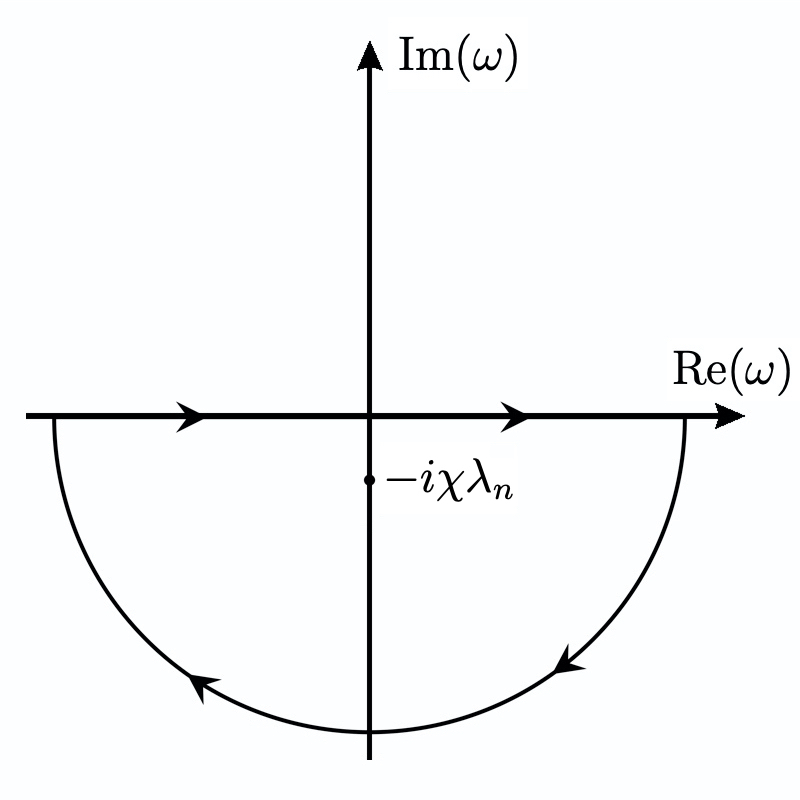
\includegraphics[width=0.45\textwidth]{immagini/complex1}
\end{center}
\[
e^{-i\omega\tau}=e^{-i(\operatorname{Re}(\omega) + i \operatorname{Im}(\omega))\tau}=e^{-i\operatorname{Re}(\omega)\tau }e^{\operatorname{Im}(\omega)\tau}
\]

Il contributo dei semicerchi all'integrale \`e nullo (come gi\`a mostrato in precedenza). %inserisci riferimento
\begin{equation}
\Rightarrow G(\tau,\x,\y)=0 \qquad \text{per } \tau<0
\label{2.80}
\end{equation}
Invece, per $\tau>0$:
\[
\int_{-\infty}^{+\infty} d\omega \frac{e^{-i\omega t}}{-i(\omega +i\chi\lambda_n)} \overset{\text{residui}}{=} 2\pi e^{-\chi \lambda_n \tau}
\]
\begin{equation}
\Rightarrow G(\tau,\x,\y)=\sum_{n} e^{-\chi\lambda_n \tau} \varphi_n (\x)\varphi_n (\y) \qquad \text{per }\tau>0
\label{2.81}
\end{equation}
$\Rightarrow$ L'equazione del calore $(\partial_t - \chi \Delta)T=S$ in $U$ ha come soluzione:
\begin{equation}
T(\x,t)=\int_0^t dt' \int_U d^d\y\, G(t-t',\x,\y)S(\y,t') + \int_U d^d\y\, G(t,\x,\y)T_0(\y)
\label{2.82}
\end{equation}
Il primo integrale \`e soluzione particolare dell'equazione non omogenea (vedi \eqref{2.78}), tenendo conto della \eqref{2.80} e di $S(\y,t')=0$ per $t'<0$.
Nota che il contributo alla temperatura al tempo $t$ viene solo dal passato ($t'<t$).

Il secondo integrale \`e  soluzione dell'equazione omogenea in modo tale che $T(\x,0)=T_0(\x)$.

\subsection{Altro esempio di applicazione del formalismo imparato}

Equazione di Laplace (Poisson) nella sfera di raggio $R$

\begin{equation}
\begin{gathered}
\Delta \phi=-F(r,\theta,\varphi) \qquad r<R\\
\phi(R,\theta,\varphi)=0
\end{gathered} 
\label{2.83}
\end{equation}
(elettrostatica: $-F=4\pi\rho$)

\[
\Delta = \partial_{r}^2 + \frac{2}{r}\partial_r + \frac{1}{r^2\sin\theta}\partial_\theta(\sin \theta \partial_\theta) + \frac{1}{r^2\sin^2\theta}\partial^2_{\varphi}
\]
Sviluppo $\phi$ in armoniche sferiche (reali):
\begin{equation}
\begin{aligned}
\phi(r,\theta,\varphi)&=\sum_{l=0}^{\infty}\Big(\overbrace{\frac{1}{2}a_{l0}(r)P^0_l(\cos\theta)}^{*} \,+\\
&+\, \sum_{m=1}^l\big(a_{lm}(r)P_l^m(\cos\theta)\cos (m\varphi) + b_{lm}(r)P_l^m (\cos\theta) \sin (m\varphi) \big)\Big) \\
F(r,\theta,\varphi)&=\sum_{l=0}^\infty\Big(\frac{1}{2} A_{l0}(r)P_l^0(\cos\theta) \,+\\
&+\, \sum_{m=1}^l \big(A_{lm}(r)P_l^m(\cos\theta)\cos (m\varphi) +B_{lm}(r)P_l^m(\cos\theta)\sin (m\varphi) \big)\Big)
\end{aligned}
\label{2.84}
\end{equation}
* N.B.: $\frac{1}{2}$ ci vuole perch\'e se no non vale \eqref{2.88} per $a_{l0}$

\smallskip

Sostituendo in \eqref{2.83}:
\[
\sum_l \Big(\frac{1}{2}a''_{l0}(r)P_l^0(\cos\theta) + \frac{2}{r}\frac{1}{2}a'_{l0}(r)P_l^0(\cos\theta) + \frac{1}{r^2}(-l)(l+1)\frac{1}{2} a_{l0}(r) P_l^0(\cos\theta) \Big) \,+
\]
\[
+\sum_{l,m>0} \Big( a''_{lm}(r)P_l^m(\cos\theta)\cos (m\varphi) + b''_{lm}(r)P_l^m(\cos\theta)\sin (m\varphi) \,+
\]
\[
+\, \frac{2}{r} a'_{lm}(r) P_l^m (\cos\theta)\cos (m\varphi) + \frac{2}{r}b'_{lm}(r)P_l^m(\cos\theta) \sin (m\varphi) \,+
\]
\[
+\, \frac{1}{r^2}a_{lm}(r)(-l)(l+1)P_l^m(\cos\theta)\cos (m\varphi) + \frac{1}{r^2} b_{lm}(r)(-l)(l+1)P_l^m(\cos\theta)\sin (m\varphi) \Big)=
\]
\[
=-\sum_l \frac{1}{2}A_{l0}(r)P_l^0(\cos\theta) - \sum_{l,m>0}\big(A_{lm}(r) P_l^m(\cos\theta)\cos (m \varphi) + B_{lm}(r)P_l^m(\cos\theta)\sin (m\varphi) \big)
\]
Avendo usato:
\[
\frac{1}{\sin\theta}\partial_\theta \Big(\sin \theta\partial_\theta \Big(P_l^m(\cos\theta) \begin{matrix}\sin m \varphi\\ \cos m \varphi \end{matrix} \Big) \Big)+\frac{1}{\sin^2\theta} \partial^2_\varphi \Big(P_l^m(\cos\theta)\begin{matrix}\sin m \varphi\\ \cos m \varphi \end{matrix} \Big)=
\]
\[
=-l(l+1)P_l^m(\cos\theta)\Big( \begin{matrix}\sin m \varphi\\ \cos m \varphi \end{matrix} \Big)
\]

Sfrutto il fatto che le armoniche sferiche $P_l^m(\cos\theta)\cos (m\varphi)$ e $P_l^m(\cos\theta)\sin (m\varphi)$ sono linearmente indipendenti:
\begin{equation} \Rightarrow \quad
\begin{gathered}
a''_{lm}(r) +\frac{2}{r}a'_{lm}(r) - \frac{l(l+1)}{r^2}a_{lm}(r)=-A_{lm}(r)\\
 b''_{lm}(r) +\frac{2}{r}b'_{lm}(r) - \frac{l(l+1)}{r^2}b_{lm}(r)=-B_{lm}(r)
\end{gathered}
\end{equation}
\[
a_{lm}(R)=b_{lm}(R)=0
\]

Entrambe le equazioni possono essere riscritte nella forma
\[
\big(pu'\big)' + qu=-f
\]
con
\[
p=r^2, \quad q=-l(l+1), \quad f=A_{lm}(r)r^2 \text{ o }B_{lm}(r)r^2, \quad u=a_{lm}(r)\text{ o }b_{lm}(r)
\]

La funzione di Green $G(r,\xi)$ soddisfa l'equazione omogenea 
\[
\frac{d}{dr}\left(r^2\frac{dG}{dr}\right)-l(l+1)G=0, \quad r\neq\xi
\]

Prova (di solito un ansatz di potenza funziona):
\[
G(r,\xi)=C(\xi)r^\alpha
\]
\[
\Rightarrow r^2\frac{dG}{dr}=C\alpha r^{\alpha+1}
\]
\[
\Rightarrow C\alpha(\alpha+1)r^\alpha - l(l+1)Cr^\alpha=0 \Rightarrow \alpha=l \vee \alpha=-l-1
\]
\[
\Rightarrow G(r,\xi)=
\begin{cases}
c_1(\xi)r^l + c_2(\xi)r^{-l-1}, & \xi\leq r\\
\tilde{c}_1(\xi)r^l + \tilde{c}_2(\xi)r^{-l-1}, & \xi \geq r
\end{cases}
\]
N.B.: L'estremo $r=0$ dell'intervallo $[0,R]$ \`e un punto singolare: $p(r)=r^2$ si annulla in $r=0$ e la soluzione fondamentale $\sim r^{-l-1}$ diverge.
Al posto di una condizione al contorno in $r=0$ richiediamo che $u$ (e $G$) rimangano limitate (richiesta fisica):
\[
\Rightarrow \tilde{c}_2=0 \text{ e }G|_{r=\xi+0}=G|_{r=\xi-0} \Rightarrow c_1\xi^l + c_2\xi^{-l-1}=\tilde{c}_1\xi^l \Rightarrow \tilde{c}_1=c_1 + c_2 \xi^{-2l-1}
\]
\[
\Rightarrow G|_{r=R}=0 \Rightarrow c_1R^l+c_2R^{-l-1}=0 \Rightarrow c_2=-c_1R^{2l + 1} \Rightarrow \tilde{c}_1=c_1(1-R^{2l+1}\xi^{-2l-1})
\]
\[
\Rightarrow G(r,\xi)=
\begin{cases}
c_1r^l \big(1-(\frac{R}{r})^{2l+1} \big), & \xi\leq r \\
c_1r^l \big(1-(\frac{R}{\xi})^{2l+1} \big), & \xi\geq r 
\end{cases}
\]
\[
\frac{dG}{dr}\Big|_{r=\xi+0}-\frac{dG}{dr}\Big|_{r=\xi-0}=-\frac{1}{p(\xi)}
\]
Questa diventa un'equazione per la variabile di integrazione $c_1$:
\[
\Rightarrow c_1=-\frac{\xi^l}{(2l+1)R^{2l+1}}
\]

\begin{equation}
\Rightarrow G_l(r,\xi)=\
\begin{cases}
\frac{1}{(2l+1)R}(\frac{\xi}{R})^l \big[(\frac{r}{R})^{-l-1} - (\frac{r}{R})^l \big], & \xi\leq r\\
\frac{1}{(2l+1)R}(\frac{r}{R})^l \big[(\frac{\xi}{R})^{-l-1} - (\frac{\xi}{R})^l \big], & \xi\geq r\\
\end{cases}
\label{2.86}
\end{equation}

\begin{equation}
\begin{gathered}
a_{lm}(r)=\int_0^r G_l(r, \xi) A_{lm}(\xi) \xi^2 d\xi \\
b_{lm}(r)=\int_0^r G_l(r, \xi) B_{lm}(\xi) \xi^2 d\xi
\end{gathered}
\label{2.87}
\end{equation}

Inversa della \eqref{2.84}:
\begin{equation}
\begin{gathered}
A_{lm}(r)=\frac{(2l+1)(l-m)!}{2\pi(l+m)!}\int_{-\pi}^\pi \int_0^\pi F(r,\theta,\varphi)P_l^m(\cos\theta) \cos (m\varphi) \sin \theta\, d\theta \,d\varphi\\
B_{lm}(r)=\frac{(2l+1)(l-m)!}{2\pi(l+m)!}\int_{-\pi}^\pi \int_0^\pi F(r,\theta,\varphi)P_l^m(\cos\theta) \sin (m\varphi) \sin \theta\, d\theta \,d\varphi
\end{gathered}
\label{2.88}
\end{equation}
(usa l'ortogonalit\`a delle armoniche sferiche $\rightarrow$ esercizio)

Con la \eqref{2.87} e \eqref{2.88}, la \eqref{2.84} diventa:
\begin{equation}
\phi(r,\theta,\varphi) =\int_{-\pi}^\pi \int_0^\pi \int_0^R G(r,\theta,\varphi,r',\theta',\varphi')F(r',\theta',\varphi')r'^2\sin\theta'dr'd\theta'd\varphi'
\label{2.89}
\end{equation}
(soluzione dell'equazione di Poisson)

dove, per $r'<r$:
\begin{equation*}
G(r,\theta,\varphi,r',\theta',\varphi')=\sum_{l,m>0}\frac{(2l+1)(l-m)!}{2\pi(l+m)!}\frac{1}{(2l+1)R}\Big(\frac{r'}{R}\Big)^l \Big[\Big(\frac{r}{R}\Big)^{-l-1}-\Big(\frac{r}{R}\Big)^l \Big]\,\cdot
\]
\[
\cdot\, P_l^m(\cos\theta)P_l^m(\cos\theta') \big(\cos (m\varphi) \cos (m\varphi')+ \sin (m\varphi) \sin (m\varphi') \big)\,+
\]
\[
+\, \sum_l \frac{1}{2}\frac{2l+1}{2\pi}\frac{1}{(2l+1)R} \Big(\frac{r'}{R}\Big)^l \Big[\Big(\frac{r}{R}\Big)^{-l-1}-\Big(\frac{r}{R}\Big)^l \Big] P^0_l (\cos \theta)P_l^0(\cos\theta')
\end{equation*}
(per $r'>r$: scambia $r$ con $r'$ in $G(r,\theta,\varphi,r',\theta',\varphi')$)

\smallskip

Si pu\`o semplificare utilizzando le propriet\`a dei polinomi di Legendre. Vedremo che il risultato si pu\`o ricavare tramite carica immagine.
\[
\sum_{m=1}^l \frac{(2l+1)(l-m)!}{2\pi(l+m)!}P_l^m(\cos\theta)P_l^m(\cos\theta')\big(\underbrace{\cos (m\varphi) \cos (m\varphi')+ \sin (m\varphi) \sin (m\varphi')}_{\frac{1}{2}\left(e^{im(\varphi - \varphi')} + e^{-im(\varphi - \varphi')}\right)}\big)\,+
\]
\[
 +\, \frac{1}{2}\frac{2l+1}{2\pi}P_l^0(\cos\theta)P_l^0(\cos\theta')=
\]
Introduco le armoniche sferiche complesse:
\[
Y_l^m(\theta,\varphi)=(-1)^m\sqrt{\frac{(2l+1)(l-m)!}{4\pi(l+m)!}}P_l^m(\cos\theta)e^{im\varphi}
\]
\[
=\sum_{m=1}^l \Big( Y_l^m(\theta,\varphi)Y_l^{m*}(\theta',\varphi') + \underbrace{Y_l^{m*}(\theta,\varphi)}_{(-1)^m Y_l^{-m}(\theta,\varphi)} \underbrace{Y_l^m(\theta',\varphi')}_{(-1)^m Y_l^{-m*}(\theta',\varphi')} \Big) + Y_l^0(\theta,\varphi)Y_l^{0*}(\theta',\varphi')=
\]
\[
=\sum_{m=-l}^l Y_l^m (\theta,\varphi)Y_l^{m*}(\theta',\varphi')=\frac{2l+1}{4\pi}P_l(\cos\gamma)
\]
con $\cos\gamma=\cos\theta\cos\theta' + \sin\theta \sin\theta' \cos(\varphi-\varphi')$. 

\begin{center}
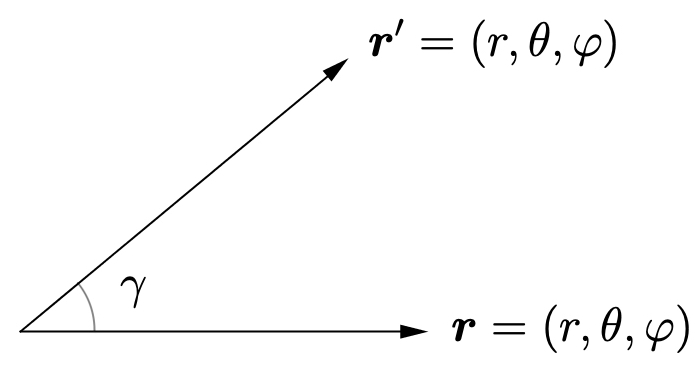
\includegraphics[width=0.4\textwidth]{immagini/vettori}
\end{center}

Quindi:
\[
G(r,\theta,\varphi,r',\theta',\varphi')=\sum_{l=0}^{\infty}\frac{1}{(2l+1)R} \Big(\frac{r'}{R}\Big)^l \Big[ \Big(\frac{r}{R}\Big)^{-l-1} - \Big(\frac{r}{R}\Big)^l\Big]\frac{2l+1}{4\pi}P_l(\cos\gamma)
\]

\begin{center}
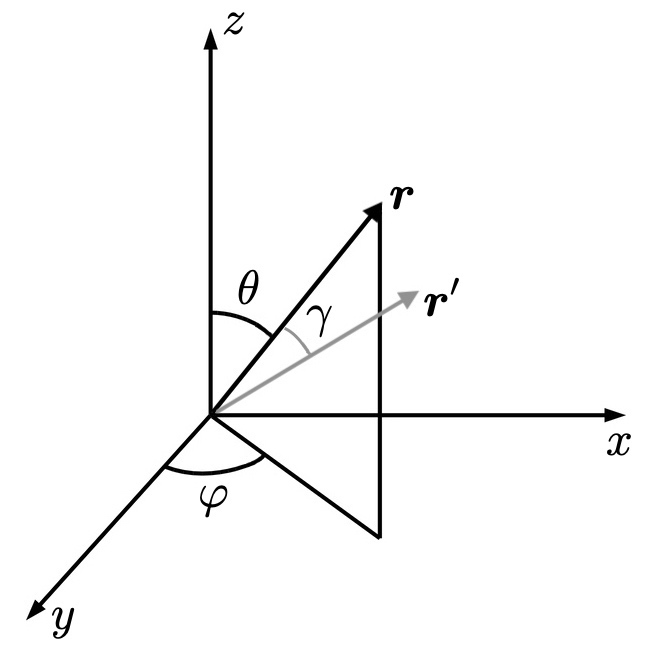
\includegraphics[width=0.4\textwidth]{immagini/vettori2-var}
\end{center}

Funzione generatrice dei polinomi di Legendre:
\begin{equation}
\frac{1}{\sqrt{1-2xt + t^2}} = \sum_{n=0}^{\infty} P_n(x)t^n
\label{2.90}
\end{equation}

\[
G(r,\theta,\varphi,r',\theta',\varphi')=\frac{1}{4\pi r} \sum_{l=0}^\infty P_l(\cos \gamma)\left(\frac{r'}{r}\right)^l - \frac{1}{4\pi R}\sum_{l=0}^\infty P_l(\cos\gamma)\left(\frac{rr'}{R^2}\right)^l=
\]
\[
\overset{\eqref{2.90}}{=}\frac{1}{4\pi r}\frac{1}{\sqrt{1-2\frac{r'}{r}\cos\gamma + \frac{r'^2}{r^2}}} - \frac{1}{4\pi R}\frac{1}{\sqrt{1-2\frac{rr'}{R^2}\cos\gamma + \frac{r^2r'^2}{R^4}}}=
\]
\begin{equation}
=\frac{1}{4\pi} \Big(r^2 + r'^2 - 2rr'\cos\gamma\Big)^{-\frac{1}{2}} - \frac{1}{4\pi}\Big(R^2 + \frac{r^2r'^2}{R^2} - 2rr'\cos\gamma\Big)^{-\frac{1}{2}} \qquad r'<r
\label{2.91}
\end{equation}
\`e gi\`a simmetrica in $r,r'$ $\rightarrow$ stesso risultato per $r' >r$.

In coordinate cartesiane:

\begin{equation}
\begin{gathered}
G(x,y,z,x',y',z')=\frac{1}{4\pi} \big\{ (x-x')^2 + (y-y')^2 + (z-z')^2 \big\}^{-\frac{1}{2}} \,+\\
-\,\frac{1}{4\pi}\frac{R}{r'} \left\{ \Big(x-x'\frac{R^2}{r'^2} \Big)^2 + \Big(y-y'\frac{R^2}{r'^2} \Big)^2 + \Big(z-z'\frac{R^2}{r'^2} \Big)^2\right\}^{-\frac{1}{2}}
\end{gathered}
\tag{$\theequation^\prime$}
\label{2.91'}
\end{equation}
dove abbiamo usato:
\[
R^2  + \frac{r^2 r'^2}{R^2} - 2rr'\cos\gamma = \frac{r'^2}{R^2}\left(r^2 + \frac{R^4}{r'^2} - \frac{2 r R^2}{r'}\cos\gamma \right)=\frac{r'^2}{R^2}(\vect{r}-\vect{\rho})^2
\]
con
\[
\vect{\rho} = \frac{R^2}{r'^2}\vect{r}'
\]

\begin{center}
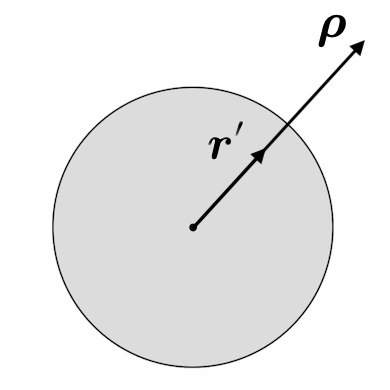
\includegraphics[width=0.3\textwidth]{immagini/palla}
\end{center}

$1^o$ termine della \eqref{2.91'}: Carica puntiforme in $\vect{r}'$

$2^o$ termine della \eqref{2.91'}: Carica immagine in $\vect{\rho} =\frac{R^2}{r'^2}\vect{r}'$ (vedi appendice \ref{caricaimm})

\section{Il kernel di Schr\"odinger}

Equazione di Schr\"odinger:

\[
i\hbar \partial_t \psi = \hat{H}\psi \overset{\text{p. libera}}{=} -\frac{\hbar^2}{2m}\Delta \psi 
\]
\begin{equation}
\Rightarrow -i\partial_t \psi =\frac{\hbar}{2m}\Delta \psi =\chi \Delta \psi 
\label{2.92}
\end{equation}
Risulta dall'equazione del calore ($\partial_t \psi =\chi \Delta \psi$) tramite la rotazione di Wick $t \rightarrow it$ 

$(\text{tempo Euclideo})$ $(\Rightarrow \partial _t \rightarrow -i\partial_t)$

Supponiamo di essere in $d$ dimensioni spaziali. 

Trasformata di Fourier:
\[
\psi(\x,t)=\frac{1}{(2\pi)^d}\int d^d\kk\, e^{i\kk\cdot \x}\tilde{\psi}(\kk,t)
\]
\[
\overset{\eqref{2.92}}{\Rightarrow} -i\partial_t \tilde{\psi}(\kk,t)=\chi (-\kk ^2)\tilde{\psi}(\kk,t)
\]
\[
\Rightarrow \tilde{\psi}(\kk,t) = e^{-i\chi\kk^2 t}\tilde{\psi}_0(\kk)
\]
con
\[
\tilde{\psi}_0(\kk)=\int d^d \y\, e^{-i\kk\cdot \y} \psi_0(\y)
\]
\[
\Rightarrow \psi(\x,t) = \frac{1}{(2\pi)^d}\int d^d \y\, \psi_0(\y) \underbrace{\int d^d\kk\, \exp\Big({i\kk \cdot (\overbrace{\x-\y}^{:=\vect{z}}) - i\chi \kk^2 t}\Big)}_{:=(2\pi)^d G(\z,t)}
\]
Riscriviamo l'esponente in modo da avere un integrale gaussiano:
\[
i\kk \cdot \z - i \chi \kk^2 t = -i\chi t\left(\kk - \frac{\z}{2\chi t}\right)^2 + \frac{i\z^2}{4\chi t}
\]
Ma attenzione: $\operatorname{Re}(i\chi t)=0$ quindi non posso risolvere l'integrale gaussiano. Dobbiamo regolarizzare con: $t\rightarrow t-i\varepsilon$, $\varepsilon>0$ e poi fare tendere $\varepsilon$ a 0. Cos\`i:
\[
\operatorname{Re}(i\chi(t-i\varepsilon))=\chi\varepsilon >0
\]
\[
\Rightarrow G(\z,t)=\frac{1}{(2\pi)^d}\exp \left(\frac{i\z^2}{4\chi(t-i\varepsilon)}\right) \int d^d\kk e^{-i\chi(t-i\varepsilon)\left( \kk -\frac{\z}{2\chi(t-i\varepsilon)}\right)^2}=
\]
\[
=\frac{1}{(2\pi)^d}\exp\left(\frac{i\z^2}{4\chi(t-i\varepsilon)}\right) \left( \frac{\pi}{i\chi(t-i\varepsilon)} \right)^\frac{d}{2}
\]
\begin{equation}
G(\z,t)\underset{\varepsilon \to 0}{\rightarrow} \left(\frac{m}{2\pi i \hbar t}\right)^{\frac{d}{2}}\exp \left(-\frac{m\z^2}{2i\hbar t}  \right)
\label{2.93}
\end{equation}
\centerline{\emph{Schr\"odinger Kernel} ($\exists\, \forall t\in \R$)}

\smallskip

Osservazione: L'equazione di Schr\"odinger \`e reversibile, quella del calore no.

Reversibile $\rightarrow$ invariante per $t \to -t$, $\psi \to \psi^*$
\[
-i\partial_t \psi =\chi \Delta \psi
\]
\[
(t\to -t)\Rightarrow i\partial_t\psi=\chi\Delta \psi
\]
\[
(\psi \to \psi^*)\Rightarrow i\partial_t\psi^*=\chi\Delta \psi^*
\]
\[
(\text{c. al contorno})\Rightarrow -i\partial_t\psi=\chi\Delta\psi
\]

Commenti:
\begin{enumerate}[label=(\roman*)]
\item $G(\x-\y,t)$ soddisfa l'equazione di Schr\"odinger $-i\partial_t G = \chi \Delta_{\x}G$
\item $\lim_{t\to 0} G(\z,t)=\delta(\z)$
\end{enumerate}

Pi\`u in generale (non necessariamente particella libera):

cerchiamo $G(\x,\y,t)$ tale che:
\begin{equation}
\psi(\x,t)=i\int d^d\y\, \psi_0(\y) G^R(\x,\y,t)
\label{2.94}
\end{equation}
$G^R(\x,\y,t)$: \emph{funzione di Green ritardata}
\[
G^R(\x,\y,t)=0 \quad \text{per }t<0
\] 

$G^R(\x,\y,t)$ rappresenta l'ampiezza di probabilit\`a che la particella vada dal punto $(\y,t=0)$ al punto $(\x,t)$ (\`e il propagatore!).

\smallskip

Troviamo $G^R(\x,\y,t)$:

$\varphi_n$ autofunzioni di $\hat{H}$:
\begin{equation}
\hat{H}\varphi_n=E_n \varphi_n 
\label{2.95}
\end{equation}

\begin{equation}
\Rightarrow G^R(\x,\y,t)=-i\sum_n e^{-iE_nt/\hbar}\varphi_n(\x)\varphi_n^* (\y), \quad t\geq 0
\label{2.96}
\end{equation}
(vedi \eqref{2.20} e \eqref{2.81})
\[
\overset{\eqref{2.94}}{\Rightarrow} \psi(\x,t)=\int d^d\y \sum_n e^{-iE_nt/\hbar}\varphi_n(\x)\varphi_n^* (\y)\psi_0(\y)
\]
e soddisfa l'equazione di Schr\"odinger, infatti:
\[
i\hbar\partial_t\psi(\x,t)=\int d^d\y \sum_n i\hbar \frac{-iE_n}{\hbar} e^{-iE_nt/\hbar}\varphi_n(\x)\varphi_n^* (\y)\psi_0(\y)
\]
e
\[
\hat{H}_{\x}\psi(\x,t)=\int d^d\y \sum_n e^{-iE_nt/\hbar}\underbrace{\hat{H}_{\x}\varphi_n(\x)}_{E_n\varphi_n(\x)} \varphi_n^* (\y)\psi_0(\y)
\]
che sono uguali.

Inoltre soddisfa il dato iniziale:
\[
\psi(\x,0)=\int d^d\y \underbrace{\sum_n \varphi_n(\x)\varphi_n^* (\y)}_{\delta(\x-\y)} \psi_0(\y)=\psi_0(\x)
\]

Se effettuiamo la trasformata di Fourier:
\[
\tilde{G}^R(\x,\y,E)=\int_{-\infty}^{+\infty}dt\, e^{iEt/\hbar}G^R(\x,\y,t)= 
\]
\[
=\int_0^\infty dt\, e^{iEt/\hbar}G^R(\x,\y,t)\overset{\eqref{2.96}}{=}-i\sum_n\int_0^\infty dt\, e^{i(E-E_n)t/\hbar}\varphi_n(\x)\varphi_n^*(\y)
\]
l'ultimo integrale non \`e ben definito se $E\in \R$ 

$\rightarrow$ Regolarizziamo tramite $E\to E+i\varepsilon$, $\varepsilon >0$
\begin{equation}
\Rightarrow \tilde{G}^R(\x,\y,E)=\sum_n\frac{\varphi_n(\x)\varphi_n^*(\y)}{E+i\varepsilon - E_n}
\label{2.97}
\end{equation}

Abbiamo:
\begin{equation}
\begin{gathered}
(E + i\varepsilon - \hat{H}_{\x})\tilde{G}^R(\x,\y,E)=\sum_n \frac{(E + i\varepsilon - \hat{H}_{\x}) \varphi_n(\x)\varphi_n^*(\y)}{E + i\varepsilon - E_n} =\\
= \sum_n \varphi_n(\x)\varphi_n^*(\y)=\delta(\x-\y)
\end{gathered}
\end{equation}
\`e il punto di partenza per le tecniche perturbative.

\medskip

\emph{Funzione di Green avanzata}: 
\[
G^A(\x,\y,t)=0 \quad \text{per } t>0
\]
Affinch\'e la trasformata di Fourier
\[
\tilde{G}^A(\x,\y,E)=\int_{-\infty}^0 dt\, e^{iEt/\hbar}G^A(\x,\y,t)
\]
esista, dobbiamo sostituire $E\to E-i\varepsilon$, $\varepsilon >0$
\[
\Rightarrow\tilde{G}^A(\x,\y,E)=\sum_n \frac{\varphi_n(\x)\varphi_n^*(\y)}{E - i\varepsilon - E_n}
\]

\medskip

\underline{Esercizio}: Calcolare $G$ per l'oscillatore armonico
\[
\hat{H}\varphi_n = -\frac{\hbar^2}{2m}\varphi''(x) + \frac{1}{2}m\omega^2 x^2 \varphi_n(x)=E_n\varphi_n(x)
\]
In meccanica quantistica abbiamo trovato $E_n=\hbar\omega\left(n+\frac{1}{2}\right)$, $n=0,1,2,\dots $, con autofunzioni date dai polinomi di Hermite:
\[
\varphi_n(x)=(\sqrt{\pi}\,2^n n!)^{-\frac{1}{2}}\exp\left(-\frac{m\omega x^2}{2\hbar}\right) \underbrace{H_n\left(\left(\frac{m\omega}{\hbar}\right)^{\frac{1}{2}}x\right)}_\text{polinomi di Hermite}
\]
\[
\eqref{2.96} \Rightarrow -i\sum_{n=0}^\infty e^{-iE_n t/\hbar}\varphi_n(x)\varphi_n^*(y)=
\]
\[
=-i\sum_{n=0}^\infty e^{-i t\omega(n+1/2)} \frac{1}{\sqrt{\pi} \, 2^n n!} \exp\left(-\frac{m\omega}{2\hbar}(x^2+y^2)\right) H_n\left(\left(\frac{m\omega}{\hbar}\right)^{\frac{1}{2}}x\right)H_n\left(\left(\frac{m\omega}{\hbar}\right)^{\frac{1}{2}}y\right)
\]
Dobbiamo quindi trovare un modo per sommare il prodotto di polinomi di Hermite.

Usa :
\begin{equation}
\sum_{n=0}^\infty \frac{H_n (x)H_n (y)}{n!} \left(\frac{u}{2}\right)^n=\frac{1}{\sqrt{1-u^2}}\exp \left\{ \frac{2u}{1+u}xy - \frac{u^2}{1-u^2}(x-y)^2 \right\}
\label{2.99}
\end{equation}
\[
\overset{u=e^{-i\omega t}}{\Rightarrow} -i\sum_{n=0}^\infty e^{-iE_n t/\hbar} \varphi_n(x)\varphi_n^*(y) = 
\]
\[
= -i e^{-i\omega t/2}\pi^{-\frac{1}{2}}\exp\left(-\frac{m\omega}{2\hbar}(x^2+y^2)\right)\frac{1}{\sqrt{1-e^{-2i\omega t}}}\cdot
\]
\[
\cdot\exp\left\{\frac{2e^{-i\omega t}}{1+e^{-i\omega t}} \frac{m\omega}{\hbar}xy - \frac{e^{-2i\omega t}}{1-e^{-2i\omega t}}\frac{m\omega}{\hbar}(x-y)^2\right\}=
\]
\begin{equation}
=-\sqrt{\frac{i}{2\pi\sin (\omega t)}}\exp\left\{ \frac{i m \omega}{\hbar}\left[\frac{x^2+y^2}{2}\cot (\omega t) - xy \operatorname{cosec} (\omega t) \right]\right\}
\label{2.100}
\end{equation}
\centerline{\emph{Mehler Kernel}}

\medskip

\underline{Esercizio}: Dimostrare che per $\omega \to 0$ la \eqref{2.100} si riduce alla \eqref{2.93} con $d=1$ (particella libera).

\section{L'equazione dei telegrafisti}

Equazioni di Maxwell nella materia (CGS):
\begin{subequations}
\begin{equation}
\operatorname{div} \vect{D} = 4\pi \rho_\text{macr.}
\label{2.101a}
\end{equation}
\begin{equation}
\operatorname{rot} \vect{H}=\frac{4\pi}{c}\vect{J}_\text{macr.} + \frac{1}{c}\frac{\partial \vect{D}}{\partial t}
\label{2.101b}
\end{equation}
\begin{equation}
\operatorname{div} \vect{B}=0 
\label{2.101c}
\end{equation}
\begin{equation}
\operatorname{rot} \vect{E}=-\frac{1}{c}\frac{\partial \vect{B}}{\partial t}
\label{2.101d}
\end{equation}
\end{subequations}

Legge di materiale (caso pi\`u semplice):
\begin{equation}
\begin{gathered}
\vect{D} = \varepsilon \vect{E} \\
\vect{B} = \mu \vect{H}
\end{gathered}
\label{2.102}
\end{equation}

Legge di Ohm:
\begin{equation}
\vect{J}_\text{macr.} = \sigma \vect{E}
\label{2.103}
\end{equation}
con $\sigma$: conducibilit\`a elettrica

\[
\eqref{2.101b}\Rightarrow \operatorname{rot} \operatorname{rot} \vect{H} = \frac{4\pi}{c} \operatorname{rot} \vect{J}_\text{macr.} + \frac{1}{c}\frac{\partial}{\partial t} \operatorname{rot} \vect{D}
\]
\[
\eqref{2.101c},\eqref{2.101d},\eqref{2.103} \Rightarrow \underbrace{ \operatorname{grad} \operatorname{div} \vect{H}}_{0} - \Delta \vect{H} = \frac{4\pi\sigma}{c}\underbrace{ \operatorname{rot} \vect{E}}_{-\frac{1}{c}\frac{\partial }{\partial t}\vect{B}} - \frac{\varepsilon}{c^2}\frac{\partial^2 \vect{B}}{\partial t^2}
\]
\begin{subequations}
\begin{equation}
\Rightarrow \Delta \vect{B}=\frac{4\pi\sigma \mu}{c^2}\frac{\partial \vect{B}}{\partial t} + \frac{\varepsilon \mu}{c^2}\frac{\partial^2 \vect{B}}{\partial t^2}
\label{2.104a}
\end{equation}
\centerline{\emph{Equazione dei telegrafisti}}

\smallskip

Detta cos\`i descrive la propagazione di un segnale nella materia (p.e. un filo).

Analogamente per $E$:
\[
\operatorname{rot} \operatorname{rot} \vect{E} = -\frac{1}{c}\frac{\partial}{\partial t} \operatorname{rot} \vect{B}=-\frac{\mu}{c}\frac{\partial}{\partial t} \operatorname{rot} \vect{H} =
\]
\[
\overset{\eqref{2.101b}}{=} -\frac{\mu}{c}\frac{\partial}{\partial t}\left(\frac{4\pi}{c}\sigma \vect{E} + \frac{\varepsilon}{c}\frac{\partial}{\partial t}\vect{E}\right)=\operatorname{grad} \operatorname{div} \vect{E} - \Delta \vect{E}
\]

se $\rho_{macr.}=0$ $\Rightarrow \operatorname{div} \vect{E}=0$

\begin{equation}
\Rightarrow \Delta \vect{E}=\frac{4\pi\sigma\mu}{c^2}\frac{\partial \vect{E}}{\partial t} + \frac{\varepsilon \mu}{c^2}\frac{\partial^2 \vect{E}}{\partial t^2}
\label{2.104b}
\end{equation}
\end{subequations}
Equivalente all'equazione delle onde, con l'aggiunta del termine dissipativo (con la derivata prima) $\rightarrow$ distrugge l'invarianza sotto inversione temporale.

\smallskip

Casi limite: 
\begin{itemize}
\item $\sigma=0$: equazione delle onde
\item $\varepsilon=0$: equazione del calore con $\chi=\frac{c^2}{4\pi \sigma \mu}$
\end{itemize}

\underline{Esercizio}: Risolvere l'equazione dei telegrafisti ($u$: qualsiasi componente di $\vect{B}$ o $\vect{E}$)
\[
\begin{gathered}
\Delta u = a\partial_t u + b \partial^2_t u \quad\text{($a,b$ costanti positive) } \\
\text{nell'intervallo}\quad 0\leq x\leq L, \quad t\geq 0 \\
\text{con}\quad u(0,t)=u(L,t)=0 \quad u(x,0)=0 \\
\frac{\partial u}{\partial t}(x,0) = g(x)
\end{gathered}
\]

Soluzione: Serie di Fourier:
\[
u(x,t)=\sum_{n=1}^\infty u_n(t) \sin \frac{n\pi x}{L}
\]
con inversa:
\[
u_n(t)=\frac{2}{L}\int_0^Lu(x,t)\sin \frac{n\pi x}{L}dx 
\]
\[
\Rightarrow -\frac{n^2\pi^2}{L^2}u_n(t)=au_n'(t) + b u_n''(t)
\]

Ansatz: $u_n(t)=\alpha_n e^{\lambda_n t}$
\[
\Rightarrow -\frac{n^2\pi^2}{L^2}=a\lambda_n + b \lambda_n^2
\]
\[
\Rightarrow \lambda_n = -\frac{a}{2b} \pm \sqrt{\frac{a^2}{4b^2}-\frac{n^2\pi^2}{L^2 b}}\equiv \lambda_n^\pm
\]
$\rightarrow$ comportamento oscillatorio se: $\frac{n^2\pi^2}{L^2}>\frac{a^2}{4b}$
\[
u_n(t)=\alpha_n^+ e^{\lambda_n^+ t} + \alpha_n^-e^{\lambda_n^- t}
\]
\[
u(x,0)=0 \Rightarrow u_n(0)=0 \Rightarrow \alpha_n^- = -\alpha_n^+
\]
\[
\Rightarrow u(x,t)=\sum_{n=1}^\infty \alpha_n^+ (e^{\lambda_n^+ t}-e^{\lambda_n^- t})\sin\frac{n\pi x}{L}
\]
\[
\frac{\partial u(x,t)}{\partial t} =\sum_{n=1}^\infty \alpha_n^+ \left(\lambda_n^+ e^{\lambda_n^+ t}-\lambda_n^-e^{\lambda_n^- t}  \right)\sin \frac{n\pi x}{L}
\]
\[
\left.\frac{\partial u(x,t)}{\partial t}\right|_{t=0}= \sum_{n=1}^\infty \alpha_n^+(\lambda_n^+ - \lambda_n^-)\sin\frac{n\pi x}{L} \overset{!}{=} g(x) = \sum_{n=1}^\infty g_n \sin \frac{n\pi x}{L}
\]
\[
\Rightarrow \alpha_n^+ = \frac{g_n}{\lambda_n^+ - \lambda_n^-}=\frac{g_n}{2\sqrt{\frac{a^2}{4b^2}-\frac{n^2\pi^2}{L^2 b}}}=\frac{1}{2\sqrt{\frac{a^2}{4b^2}-\frac{n^2\pi^2}{L^2 b}}} \frac{2}{L}\int_{0}
^{L}g(x')\sin\frac{n\pi x'}{L} dx'
\]
e quindi:
\[
u(x,t)=\frac{1}{L}\int_0^L dx' \sum_{n=1}^\infty \frac{e^{\lambda_n^+ t} - e^{\lambda_n^- t}}{\sqrt{\frac{a^2}{4b^2}-\frac{n^2\pi^2}{L^2 b}}}\sin\frac{n\pi x'}{L}\sin \frac{n\pi x}{L}g(x')
\]
\[
\Rightarrow u(x,t)=\int_0^L G(x,x',t)g(x')dx'
\]
Con la funzione di Green
\[
G(x,x',t)=\frac{1}{L} \sum_{n=1}^\infty \frac{e^{\lambda_n^+ t} - e^{\lambda_n^- t}}{\sqrt{\frac{a^2}{4b^2}-\frac{n^2\pi^2}{L^2 b}}}\sin\frac{n\pi x'}{L}\sin \frac{n\pi x}{L}
\]

N.B.: Se esiste $n_0$ tale che $\lambda_{n_0}^+ = \lambda_{n_0}^-$ (cio\`e $\sqrt{\frac{a^2}{4b^2}-\frac{n^2\pi^2}{L^2 b}}=0$):

Scrivi
\[
\frac{e^{\lambda_n^+ t} - e^{\lambda_n^- t}}{\sqrt{\dots}}= \frac{e^{\left(-\frac{a}{2b}+\sqrt{\dots}\right)t}- e^{\left(-\frac{a}{2b}-\sqrt{\dots}\right)t}}{\sqrt{\dots}}=
\]
\[
=\frac{e^{-\frac{at}{2b}} 2\sinh (\sqrt{\dots} t)}{\sqrt{\dots}} \xrightarrow{\sqrt{\cdots}\to 0} \frac{e^{-\frac{at}{2b}}2\sqrt{\cdots}t}{\sqrt{\cdots}}=2te^{-\frac{at}{2b}}
\]
cio\`e basta escludere $n_0$ dalla somma e sostituirci questo.

\section{Classificazione delle equazioni differenziali alle derivate parziali lineari del secondo ordine}

Per semplicit\`a ci limitiamo alle equazioni in 2 variabili
\begin{equation}
a_{11}(x,y)u_{xx} + 2a_{12}(x,y)u_{xy} + a_{22}(x,y)u_{yy} + b_{1}(x,y)u_{x} + b_2(x,y)u_y + c(x,y)u = d(x,y)
\label{2.105}
\end{equation}

La classificazione \`e basata solo sulla parte contenente le derivate seconde, $a_{11}u_{xx} + 2a_{12}u_{xy} +a_{22}u_{yy}$, detta \emph{parte principale} dell'equazione.

\smallskip

\underline{Definizione}: Sia $\delta(x,y)=a_{12}^2 - a_{11}a_{22}$, il \emph{discriminante} della parte principale.
\begin{itemize}
\item se $\delta >0$ l'equazione \eqref{2.105} si dice \emph{iperbolica}
\item se $\delta =0$ l'equazione \eqref{2.105} si dice \emph{parabolica}
\item se $\delta <0$ l'equazione \eqref{2.105} si dice \emph{ellittica}
\end{itemize}
N.B.: La definizione si estende anche alle equazioni \emph{quasilinearli} (nelle quali i coefficienti $a_{ij}$ possono dipendere anche da $u$, $u_x$, $u_y$) se si riesce a stabilire il segno di $\delta$.

\medskip

\underline{Esempio} quasilineare: \emph{Equazione delle superfici minime}

Considera la superficie in $\R^3$ definita da $z=u(x,y) : (x,y) \in \Omega \subset \R^2$
\begin{center}
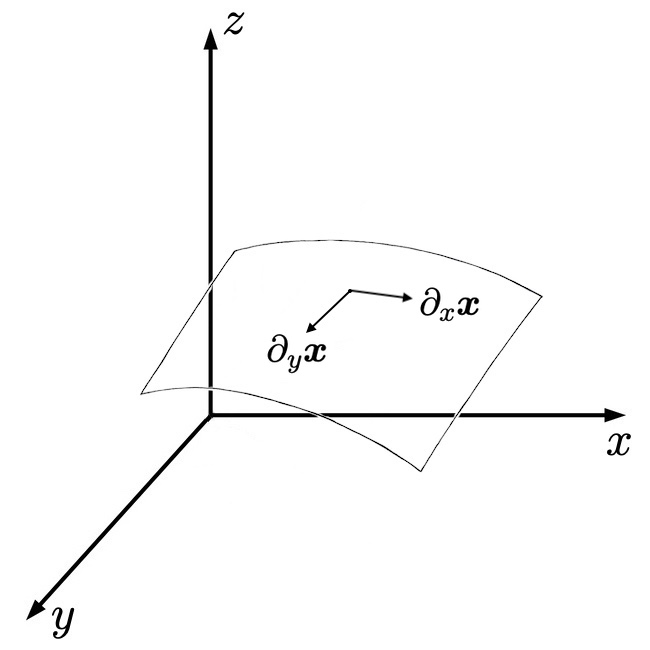
\includegraphics[width=0.4\textwidth]{immagini/superficie}
\end{center}
\[
\x = \left( \begin{matrix}
x\\
y\\
u(x,y)
\end{matrix}\right) \in \R^3
\]
Fissato il bordo della superficie, qual \`e la condizione su $x,y$ affinch\'e l'area sia minima?

Prima si calcola l'area $\rightarrow$ servono i vettori tangenti:
\[
\partial_x \x = \frac{\partial \x}{\partial x} =\left( \begin{matrix}
1\\
0\\
u_x
\end{matrix}\right) ,\quad 
\partial_y \x = \frac{\partial \x}{\partial y} =\left( \begin{matrix}
0\\
1\\
u_y
\end{matrix}\right)
\]
\centerline{(vettori tangenti)}
con $u_x=\frac{\partial u}{\partial x}$, $u_y=\frac{\partial u}{\partial y}$.

\[
\vect{N}=\frac{\partial \x}{\partial x} \times \frac{\partial \x}{\partial y}=\left| \begin{matrix}
\vect{e}_x & \vect{e}_y & \vect{e}_z \\
1 & 0 & u_x \\
0 & 1 & u_y
\end{matrix}\right| = \vect{e}_z-u_x \vect{e}_x - u_y \vect{e}_y = \left( \begin{matrix}
-u_x \\
-u_y \\
1
\end{matrix}\right)
\]
\centerline{(vettore normale)}

\[
\Rightarrow dA = |\vect{N}|dxdy=\sqrt{u_x^2 + u_y^2 +1}dxdy 
\]
\centerline{(elemento di superficie)}

$\Rightarrow$ area della superficie:
\begin{equation}
A=\int_{\Omega} \sqrt{1+(\nabla u)^2} dxdy\equiv \int_{\Omega} \mathcal{L}dxdy (106)
\end{equation}

Superfici minime: $\delta A=0$ (principio variazionale)

Equazioni di Eulero-Lagrange:
\begin{equation}
\frac{\partial}{\partial x_i}\left( \frac{\partial \mathcal{L}}{\partial (\frac{\partial u}{\partial x_i})} \right)-\frac{\partial \mathcal{L}}{\partial u}=0
\label{2.107}
\end{equation}
Si sottintende la somma su $i$ da 1 a 2

\[
\frac{\partial}{\partial x_i}:=\partial_i \Rightarrow \frac{\partial\mathcal{L}}{\partial \partial_i u} = \frac{1}{2} \big(1 +(\nabla u)^2\big)^{-\frac{1}{2}} 2\partial_i u=\frac{\partial_i u}{\sqrt{(1+(\nabla u)^2}}, \qquad \frac{\partial \mathcal{L}}{\partial u}=0 
\]
\[
\eqref{2.107}\Rightarrow \partial_i \left( \frac{\partial_i u}{\sqrt{1+(\nabla u)^2}}\right)=0
\]
che si scrive anche
\begin{equation}
\nabla \cdot \left( \frac{\nabla u}{\sqrt{1+(\nabla u)^2}}\right)=0
\label{2.108}
\end{equation}
\centerline{\emph{Equazione delle superfici minime}}

In alternativa alle equazioni di Eulero-Lagrange \eqref{2.107}:
\[
\delta\mathcal{L}=\delta\sqrt{1+(\nabla u)^2}=\frac{1}{2}\big(1+(\nabla u)^2\big)^{-\frac{1}{2}}2\nabla u \nabla \delta u
\]
Integro per parti e tengo conto di $\delta u\big|_\text{bordo}=0$

Come in meccanica: $L=\frac{1}{2} m x^2$, $\delta L = m \dot{x} \delta \dot{x} \rightarrow -m \ddot{x} \delta x$
\[
\rightarrow -\delta u \nabla \cdot \left(\frac{\nabla u}{\sqrt{1+(\nabla u)^2}}\right)\overset{!}{=}0 \quad \forall \delta u \Rightarrow \eqref{2.108}
\]
\[
\eqref{2.108} \Rightarrow \frac{\partial_i \partial_i u}{\sqrt{1+(\nabla u)^2}} + \partial_i u \left(-\frac{1}{2}\right) \big(1+(\nabla u)^2\big)^{-\frac{3}{2}} \underbrace{\partial_i (\nabla u)^2}_{ \substack{\partial_i(\partial_j u \partial_j u)= \\ =2(\partial_i\partial_j u)\partial_j u } } =0
\]
\[
\Rightarrow \big(1+ (\nabla u)^2 \big) \Delta u - \partial_x u \partial_x u \partial_x^2 u - \partial_x u\partial_y u \partial_x\partial_y u - \partial_yu \partial_x u \partial_y \partial_x u - \partial_y u\partial_y u \partial_y^2 u =0
\]
e poich\'e $(\nabla u)^2=(\partial_x u)^2 + (\partial_y u)^2$ e $\Delta u =\partial_x^2 u + \partial_y^2 u$
\[
\Rightarrow u_{xx} + u_{yy} + u_x^2 u_{yy} + u_y^2 u_{xx} - 2u_xu_y u_{xy}=0
\]
\begin{equation}
\Rightarrow (1+u_y^2)u_{xx} + (1+u_x^2) u_{yy} - 2u_x u_y u_{xy}=0 
\tag{$\theequation^\prime$}
\label{2.108'}
\end{equation}
\[
\Rightarrow a_{11}=1+u_y^2, \qquad a_{22}=1+u_x^2, \qquad a_{12}=-u_x u_y
\]
Posso calcolare il discriminante:
\[
\delta = a_{12}^2 -a_{11}a_{22} = u_x^2 u_y^2 - (1+u_x^2 + u_y^2 + u_x^2u_y^2)=-(1+(\nabla u)^2) <0
\]
\centerline{$\Rightarrow$ equazione ellittica}
\centerline{\emph{Equazione di Young-Laplace}}

Definisco la matrice $ A:=\left(\begin{matrix}
a_{11} & a_{12}\\
a_{12} & a_{22}
\end{matrix}\right)$, $\det A=-\delta$
\begin{itemize}
\item Iperbolica ($\delta >0$): $\det A<0$, 2 autovalori di segno opposto
\item Parabolica ($\delta =0$): 1 autovalore=0 (altrimenti banale)
\item Ellittica ($\delta <0$): 2 autovalori di segno uguale
\end{itemize}
\`E il parallelismo con il comportamento della forma quadratica generata da $A$ a suggerire la medesima denominazione delle coniche.

\underline{Esempi}:

\begin{itemize}
\item Equazioni ellittiche: Laplace, Poisson (parte principale $\Delta u$)
\item Equazioni paraboliche: Equazione del calore $\partial_t u = \chi \partial_x^2 u$ ($y \leftrightarrow t$)
\item Equazioni iperboliche: Equazione delle onde e dei telegrafisti (quest'ultima per $\epsilon \neq 0$, altrimenti parabolica), equazione di Klein-Gordon
\end{itemize}

\section{Il problema di Cauchy}
La classificazione ha una prima motivazione nel problema di Cauchy: trovare una funzione $u\in C^2$ che soddisfi la \eqref{2.105} e i dati di Cauchy, ossia:
\begin{equation}
u \big|_{\gamma}=\Phi \big|_{\gamma}, \quad \frac{\partial u}{\partial n} \Big|_{\gamma}=\Psi \big|_{\gamma}
\label{2.109}
\end{equation}

dove $\Phi$, $\Psi$ sono funzioni assegnate e $\gamma$ \`e una data curva regolare con normale $\vect{n}$, $\frac{\partial u}{\partial n}=\vect{n}\cdot \nabla u$.

%immagine curva regolare con normale%

Possibile modo di tentare di risolvere il problema: supporre che le $a_{ij}$, la $\gamma$ e i dati $\Phi$, $\Psi$ siano analitici e cercare:
\begin{enumerate}[label=(\roman*)]
\item di calcolare tutte le derivate di $u$ su $\gamma$
\item di dimostrare che lo sviluppo di Taylor di $u$ \`e convergente in un intorno di $\gamma$.
\end{enumerate}
Se il procedimento ha successo si \`e costruita una soluzione analitica.

Questo \`e l'obiettivo del \emph{teorema di Cauchy-Kowalevski}: 

Se i coefficienti $a_{ij}$, $b_i$, c, d sono tutti analitici in un dominio $D$, se la curva $\gamma \subset D$ \`e analitica e i dati di Cauchy $\Phi$, $\Psi$ sono analitici in $D$, il problema di Cauchy \eqref{2.105}, con dati iniziali \eqref{2.109}, ammette una e una sola soluzione analitica in un opportuno intorno $I\subset D$ di $\gamma$, purch\'e la normale $\vect{n}$ a $\gamma$ verifichi la condizione 
\begin{equation}
\vect{n}\cdot A \vect{n}\neq 0
\label{2.110}
\end{equation}
(senza dim.)

$\rightarrow$ la \eqref{2.110} chiama in causa la classificazione.
Il ruolo della \eqref{2.110} \`e quello di consentire il calcolo delle derivate seconde:
\[
\vect{n}\equiv (\alpha,\beta)
\]

%immagine derivata tangenzialmente gamma%

Deriva tangenzialmente il primo dato di Cauchy:
\[
\left.\frac{\partial u}{\partial \tau}\right|_{\gamma} = \left. \frac{\partial \Phi}{\partial \tau}\right|_{\gamma}, \qquad
\frac{\partial}{\partial \tau} \equiv \vect{\tau}\cdot \nabla, \qquad 
\vect{\tau}= (-\beta,\alpha), \qquad 
\alpha^2 + \beta^2 =1
\]
\begin{equation}
\Rightarrow (-\beta u_x +\alpha u_y) \big|_{\gamma}=\left.\frac{\partial \Phi}{\partial \tau}\right|_{\gamma}
\label{2.111}
\end{equation}
Secondo dato di Cauchy:
\begin{equation}
(\alpha u_x + \beta u_y) \big|_{\gamma} = \Psi|_{\gamma}
\label{2.112}
\end{equation}
\`E un sistema lineare non omogeneo in $u_x$ e $u_y$.
La matrice dei coefficienti \`e $\left( \begin{matrix} -\beta & \alpha \\ \alpha & \beta \end{matrix} \right)$ che ha sempre determinante$\neq0$

$\rightarrow$ \eqref{2.111}, \eqref{2.112} $\underset{\alpha^2 + \beta^2 \neq 0}{\implies} u_x \big|_{\gamma}=p_0(s)$
\begin{equation}
u_y \big|_{\gamma}=q_0(s)
\label{2.113}
\end{equation}
dove $p_0$, $q_0$ sono espresse tramite i dati e $s$ \`e il parametro naturale su $\gamma$ (lunghezza della curva).

Servono ora le derivate seconde.

Deriva \eqref{2.113} lungo $\gamma$:
\[
\vect{\tau}\cdot \nabla u_x \big|_{\gamma}= p_0'(s)
\]
\[
\vect{\tau}\cdot \nabla u_y \big|_{\gamma}=q_0'(s)
\]
\[
\Updownarrow
\]
\[
\begin{cases}
(-\beta u_{xx} + \alpha u_{xy}) \big|_{\gamma}=p_0'\\
(-\beta u_{xy} + \alpha u_{yy}) \big|_{\gamma}=q_0'
\end{cases}
\]

La parte principale nella \eqref{2.105} \`e esprimibile su $\gamma$ in base ai dati, perch\'e tutti i termini rimanenti sono calcolabili:
\[
(a_{11}u_{xx}+2a_{12}u_{xy}+a_{22}u_{yy}) \big|_{\gamma}=r_0(s)
\]
$\Rightarrow$ sistema di 3 equazioni lineare con determinante
\begin{equation}
\left| \begin{matrix}
a_{11} & 2a_{12} & a_{22}\\
-\beta & \alpha & 0 \\
0 & -\beta & \alpha 
\end{matrix}\right| = \vect{n}\cdot A \vect{n}
\label{2.114}
\end{equation}
$\Rightarrow$ la condizione \eqref{2.110} consente di calcolare le derivate seconde. Nello stesso modo si calcolano, sempre grazie alla \eqref{2.110}, tutte le derivate successive.

Interpretazione geometrica della (negazione della) \eqref{2.110}:

\begin{equation}
\vect{n}\cdot A\vect{n}=a_{11}\alpha^2+2a_{12}\alpha\beta + a_{22}\beta^2=0
\label{2.115}
\end{equation}
Autovalori di $A$: $\underbrace{\lambda_1,\lambda_2}_{\in\R}$; con autovettori ortogonali $\vect{\theta}_1,\vect{\theta}_2$ ($A$ simmetrica)
\[
\vect{n}:= \eta_1 \vect{\theta}_1 + \eta_2\vect{\theta}_2 \Rightarrow \vect{n}\cdot A \vect{n}=\lambda_1\eta_1^2 + \lambda_2\eta_2^2
\]
\begin{itemize}
\item Caso ellittico: sempre $\neq 0$.
\item Caso parabolico: $A\vect{n}=0$ per $\vect{n}$ nell'autospazio corrispondente all'autovalore nullo.
\item Caso iperbolico: $\vect{n}\cdot A\vect{n} = 0$ per $\frac{\eta_1}{\eta_2}=\pm \sqrt{\left|\frac{\lambda_1}{\lambda_2}\right|}$
\end{itemize}
$\rightarrow$ 2 campi vettoriali
\[
\vect{w}_1 = \sqrt{|\lambda_2|}\vect{\theta}_1 + \sqrt{|\lambda_1|}\vect{\theta}_2, \qquad (\eta_2=\sqrt{|\lambda_1|},\, \eta_1=\sqrt{|\lambda_2|})
\]
\[
\vect{w}_2 = \sqrt{|\lambda_2|}\vect{\theta}_1 + \sqrt{|\lambda_1|}\vect{\theta}_2, \qquad (\eta_2=\sqrt{|\lambda_1|},\, \eta_1=-\sqrt{|\lambda_2|})
\]
Curve $\perp$ a questi campi: $\chi_{1,2}(x,y)=\text{cost}$

%immagine curva perp%

\[
\Rightarrow \vect{n} \propto \nabla\chi \Rightarrow (\alpha,\beta) \propto (\chi_x, \chi_y)
\]
e quindi:
\begin{equation}
\eqref{2.115} \Rightarrow a_{11}\chi_x^2 + 2a_{12}\chi_x\chi_y + a_{22}\chi_y^2 =0
\label{2.116}
\end{equation}
Poni $\chi := f(x)-y$ (si pu\`o fare perch\'e $f(x)-y=cost \Rightarrow y=f(x) - cost$ cio\`e perch\'e $\chi(x,y)=cost$ la posso sempre risolvere per ottenere $y$ in funzione di $x$)
\[
\Rightarrow \chi_x = f', \quad \chi_y=-1
\]
\begin{equation}
\eqref{2.116}\Rightarrow a_{11}f'^2 - 2 a_{12}f' + a_{22}=0
\label{2.116'}
\tag{$\theequation^\prime$}
\end{equation}
$\rightarrow$ equazione di secondo grado per $f'$

Nel caso parabolico ci si riduce ad una sola famiglia, nel caso ellittico non ci sono curve di questo genere.

\medskip

\underline{Definizione}: Le curve $\chi(x,y)=cost$ soddisfacenti la \eqref{2.116} si chiamano \emph{curve caratteristiche} dell'equazione \eqref{2.105}

Esempi:
\begin{enumerate}[label=(\roman*)]
\item equazione d'onda in 1+1 dimensioni
\[
c^2 u_{xx}-u_{tt}=0, \qquad a_{11}=c^2, \quad a_{12}=0, \quad a_{22}=-1
\]
\[
\eqref{2.116'}\Rightarrow c^2f'^2 =1 \Rightarrow f=\pm \frac{x}{c} + f_0
\]
\[
\chi=f(x) - t= \pm \frac{x}{c}+f_0 -t \overset{!}{=}cost
\]
\[
\Rightarrow x-x_0 \pm c(t-t_0)=0 \qquad \text{(cono luce)}
\]
%disegno del cono di luce
\item equazione del calore 
\[
\chi u_{xx}- u_t=0
\]
\[
\Rightarrow a_{11}=\chi, \quad a_{12}=a_{22}=0
\]
\[
\eqref{2.116'} \Rightarrow \chi f'^2 =0 \Rightarrow f=cost=:f_0
\]
\[
\chi = f_0-t \overset{!}{=} cost \Rightarrow t = cost \quad \text{(retta)}
\]
\end{enumerate}
Cambiamento di coordinate:

Sia $\xi=\xi(x,y)$, $\eta=\eta(x,y)$ un cambiamento di coordinate con determinante Jacobiano $\neq 0$.
\[
v(\xi,\eta):=u(x,y)
\]
Come si trasforma la parte principale della \eqref{2.105}?
\[
u_x=v_\xi \xi_x + v_\eta \eta_x
\]
\[
u_y=v_\xi \xi_y + v_\eta \eta_y
\]
\[
u_{xx}=v_{\xi \xi}\xi_x^2 + 2v_{\xi\eta}\xi_x\eta_x + v_{\eta\eta}\eta_x^2 + v_\xi \xi_{xx} +v_\eta \eta_{xx}
\]
\[
u_{xy}= v_{\xi \xi}\xi_x\xi_y + v_{\xi\eta}(\xi_x\eta_y + \xi_y\eta_x) + v_{\eta\eta} \eta_x\eta_y + v_\xi \xi_{xy} + v_\eta \eta_{xy}
\]
\[
u_{yy}= v_{\xi\xi }\xi_y^2 + 2v_{\xi\eta}\xi_y\eta_y + v_{\eta\eta}\eta_y^2 + v_\xi \xi_{yy} + v_\eta \eta_{yy}
\]
%\[ \frac{\partial}{\partial x} = \frac{\partial \xi}{\partial x}\frac{\partial}{\partial \xi} + \frac{\partial \eta}{\partial x}\frac{\partial}{\partial \eta} \]
%\[ \frac{\partial}{\partial y} = \frac{\partial \xi}{\partial y}\frac{\partial}{\partial \xi} + \frac{\partial \eta}{\partial y}\frac{\partial}{\partial \eta} \]
$\rightarrow$ la parte principale della \eqref{2.105} diventa: 
\[
\tilde{a}_{11} v_{\xi\xi} + 2 \tilde{a}_{12}v_{\xi\eta} + \tilde{a}_{22}v_{\eta\eta}
\]
con 
\[
\tilde{a}_{11}= a_{11} \xi_x^2 + 2a_{12}\xi_x\xi_y + a_{22} \xi_y^2 = \nabla\xi \cdot A \nabla \xi
\]
\[
\tilde{a}_{12}= a_{11} \xi_x\eta_x + a_{12}(\xi_x\eta_y+\xi_y\eta_x) + a_{22} \xi_y\eta_y = \nabla \eta \cdot A\nabla \xi = \nabla \xi \cdot A \nabla \eta
\]
\[
\tilde{a}_{22}= a_{11} \eta_x^2 + 2a_{12}\eta_x\eta_y + a_{22} \eta_y^2 = \nabla \eta \cdot A \nabla \eta
\]
\begin{equation}
\Rightarrow \tilde{A} = J A J^{-1} \qquad J=\text{Jacobiano} 
\label{2.117}
\end{equation}
\[
\Rightarrow \det \tilde{A} = \det A (\det J)^2
\]
$\Rightarrow$ le trasformazioni invertibili di coordinate lasciano invariante il carattere dell'equazione.

\underline{Esempio}: Equazione d'onda $c^2u_{xx} - u_{tt}=0$.

Prendi $\xi=x-ct$, $\eta = x+ct$, (coordinate di cono luce) e poni $v(\xi,\eta) = u(x,y)$ 

$\Rightarrow \tilde{A}=\left(\begin{matrix} 0 & 1\\ 1 & 0 \end{matrix}\right)$ e l'equazione diventa $v_{\xi\eta}=0$. 

$\Rightarrow$ Soluzione generale:
\[
v(\xi,\eta)=f(\xi) + g(\eta) \quad \text{(con $f$, $g$ funzioni arbitrarie)}
\]
Questo puoi farlo solo in 1+1 dimensioni

Riduzione alla forma canonica:

forme canoniche:
\begin{itemize}
\item[] $u_{xx} + u_{yy} \quad$ ellittica
\item[] $u_{xx} (- u_t) \quad$ parabolica
\item[] $u_{xx} - u_{tt} \quad$ iperbolica (in alternativa $u_{xt}$)
\end{itemize}
N.B.: Costanti come per esempio $c^2$ in $c^2 u_{xx}-u_{tt}$ possono essere riassorbite nella scala delle variabili:
\[
c^2 \frac{\partial^2 u}{\partial x^2} \overset{x\to cx}{\longrightarrow} \frac{\partial^2 u}{\partial x^2}
\]
Trasformazione di una parte principale generica nella forma canonica:

\medskip

\emph{Caso iperbolico}:

L'esempio sopra suggerisce di prendere le curve caratteristiche come nuove linee coordinate 
\[
\xi=\chi_1(x,y),\quad \eta=\chi_2(x,y)
\]
\[
\eqref{2.117}\Rightarrow \tilde{A} = \left(\begin{matrix}
\tilde{A}_{11} & \tilde{A}_{12} \\
\tilde{A}_{21} & \tilde{A}_{22}
\end{matrix} \right)\overset{\eqref{2.116}}{=}\left(\begin{matrix}
0 & *\\
* & 0
\end{matrix}\right)
\]

$\tilde{A}_{11}=a_{11}\chi_{1x}^2 + 2a_{12}\chi_{1x}\chi_{1y} + a_{22}\chi_{1y}^2$

$\tilde{A}_{12}=\tilde{A}_{21}=a_{11}\chi_{1x}\chi_{2x} + a_{12}(\chi_{1x}\chi_{2y} + \chi_{1y}\chi_{2x}) + a_{22}\chi_{1y}\chi_{2y}$

$\tilde{A}_{22}=a_{11}\chi_{2x}^2 + 2a_{12}\chi_{2x}\chi_{2y} + a_{22}\chi_{2y}^2$

$\rightarrow$ parte principale riconducibile alla forma canonica $u_{xy}$ 

($2 * v_{\xi\eta} + (\text{derivate dell'ordine }\leq1) =0$ dividi per $* \Rightarrow 2v_{\xi \eta}$ per parte principale)

\medskip

\emph{Caso parabolico}:

prendi $\xi=x$, $\eta=\chi(x,y)$
\[
\Rightarrow J=\left(\begin{matrix}
\xi_x & \xi_y \\
\eta_x & \eta_y
\end{matrix}\right)=\left( \begin{matrix}
1 & 0\\
\chi_{x} & \chi_y
\end{matrix}\right)
\]

N.B.: $\det A=0 \Rightarrow$ Se uno dei coefficienti $a_{11}, a_{22}$ \`e nullo lo \`e anche $a_{12}$ ($a_{11}a_{22}-a_{12}^2=0$). In tal caso siamo già nella forma canonica.

$\rightarrow $ supponiamo $a_{11}a_{22}>0$ ( non pu\`o essere $<0$, perch\'e $a_{12}^2 = a_{11}a_{22}$).

Equazione delle caratteristiche \eqref{2.116}:
\[
a_{11}\chi_x^2+2\sqrt{a_{11}a_{22}}\chi_x\chi_y + a_{22}\chi_y^2 =0
\]
(se $a_{12}=-\sqrt{a_{11}a_{22}}$: manda $y$ in $-y$).

Inoltre, senza perdere la generalit\`a: $a_{11}>0$ (altrimenti moltiplica la \eqref{2.105} con -1) $\Rightarrow a_{22}>0$.

$\rightarrow$ abbiamo $(\sqrt{a_{11}}\chi_x + \sqrt{a_{22}}\chi_y)^2=0$
\begin{equation}
\Rightarrow\chi_y = - \sqrt{\frac{a_{11}}{a_{22}}}\chi_x
\label{2.118}
\end{equation}
\[
\tilde{A}=\left(\begin{matrix}
1 & 0\\
\chi_x & \chi_y
\end{matrix}\right)\left(\begin{matrix}
a_{11} & \sqrt{a_{11}a_{22}}\\
\sqrt{a_{11}a_{22}} & a_{22}
\end{matrix}\right)\left(\begin{matrix}
1 & \chi_x \\
0 & \chi_y
\end{matrix}\right)=
\]
\[
=\left(\begin{matrix}
a_{11} & a_{11}\chi_x + \sqrt{a_{11}a_{22}}\chi_y \\
a_{11}\chi_x + \sqrt{a_{11}a_{22}}\chi_y & a_{11}\chi_x^2 + 2\sqrt{a_{11}a_{22}}\chi_x\chi_y + a_{22}\chi_y^2
\end{matrix}\right)\overset{\eqref{2.118}}{=}\left(\begin{matrix}
a_{11} & 0\\
0 & 0
\end{matrix}\right)
\]

$\rightarrow$ forma canonica

\medskip

\emph{Caso ellittico}:

Il metodo seguito per le equazioni iperboliche e paraboliche non \`e applicabile (non disponiamo di curve caratteristiche)

$\rightarrow$ torna alla \eqref{2.117} e imponi direttamente $\tilde{a}_{12}=0$, $\tilde{a}_{11}=\tilde{a}_{22}$
\begin{equation}
a_{11}\xi_x \eta_x + a_{12}(\xi_x\eta_y + \xi_y\eta_x) + a_{22}\xi_y\eta_y=0
\label{2.119}
\end{equation}
\begin{equation}
a_{11}(\xi_x^2 - \eta_x^2) + 2a_{12}(\xi_x\xi_y - \eta_x\eta_y) + a_{22}(\xi_y^2 - \eta_y^2)=0
\label{2.119'}
\tag{$\theequation^\prime$}
\end{equation}
$2i\eqref{2.119} + \eqref{2.119'}$:
\begin{equation}
\Rightarrow a_{11}(\xi_x + i\eta_x)^2 + 2a_{12}(\xi_x + i\eta_x)(\xi_y + i\eta_y) + a_{22}(\xi_y + i\eta_y)^2 =0
\label{2.119''}
\tag{$\theequation^{\prime\prime}$}
\end{equation}
Si ha: $a_{11}a_{22}>0$ nel caso ellittico (altrimenti $\delta =a_{12}^2 - a_{11}a_{22}$ non pu\`o essere $<0$). 

$\rightarrow$ la \eqref{2.119''} \`e un'equazione di secondo grado non degenere per $\rho:= \frac{\xi_x + i\eta_x}{\xi_y + i\eta_y}$, con soluzioni $\rho_{\pm}=-\frac{\left(a_{12} \pm i\sqrt{|\delta|} \right)} { a_{11}}$

Prendi per esempio $\rho_+$:
\[
\Rightarrow a_{11} (\xi_x + i\eta_x)=-(a_{12}+i\sqrt{|\delta|})(\xi_y + i \eta_y)
\]
e quindi 
\begin{equation}
\begin{cases}
\xi_x=\frac{(a_{12}\eta_x + a_{22}\eta_y)}{\sqrt{|\delta|}} \\
\xi_y=\frac{-(a_{11}\eta_x + a_{12}\eta_y)}{\sqrt{|\delta|}}
\end{cases}
\label{2.120}
\end{equation}
\centerline{\emph{Equazioni di Beltrami}} 

Caratterizzano le trasformazioni che conducono la parte principale ad un'espressione proporzionale all'operatore di Laplace. \`E stato dimostrato (risultato non banale) che le \eqref{2.120} ammettono soluzioni nell'intera regione di ellitticit\`a.

N.B.: Le \eqref{2.120} possono essere scritte nella forma:
\begin{equation}
\frac{\partial w}{\partial \z}=\mu\frac{\partial w}{\partial z}
\label{2.120'}
\tag{$\theequation^\prime$}
\end{equation}
con $z=x+iy$, $w=\xi+i\eta$, $\mu=\frac{a_{11}+i a_{12} - \sqrt{|\delta|}}{-a_{11}+i a_{12} - \sqrt{|\delta|}}$ (esercizio)

Commento: Una mappa $w(z,\z)$ che soddisfa la \eqref{2.120'} viene chiamata mappa \emph{quasi-conforme}

(Caso particolare $\mu=0$: mappa conforme, $w=w(z)$ funzione olomorfa).

\subsection{La questione della buona posizione del problema di Cauchy}

\underline{Definizione}: Un problema al contorno per un equazione alle derivate parziali di dice \emph{ben posto secondo Hadamard} se possiede una e una sola soluzione ed essa dipende in modo continuo dai dati iniziali.

Commenti:
\begin{enumerate}[label=(\roman*)]
\item L'enunciato corretto di un problema al contorno contiene non soltanto l'equazione differenziale e i dati al contorno, ma anche la prescrizione dello spazio funzionale in cui si cerca la soluzione. Questa scelta \`e in grado di influenzare ad esempio l'unicit\`a.

\item Cosa si intende per dipendenza continua? $\rightarrow$ richiede una metrica nello spazio delle soluzione e una metrica nello spazio dei dati

$X$: spazio delle soluzioni, con norma $\| \cdot \|_X$

$Y$: spazio dei dati, con norma $\| \cdot \|_Y$
\end{enumerate}
Dipendenza continua significa:

Sia $\{\vect{\delta}_n\}$ successione di dati (ordinabili in un vettore) tale che  $\lim_{n\to\infty} \| \vect{\delta}_n - \vect{\delta}\|_Y=0$ e sia $\{u_n\}$ una successione di soluzioni. $u$: soluzione corrispondente al dato limite $\vect{\delta}$.

Si ha dipendenza continua se:
\[
\lim_{n\to \infty}\|u_n - u \|=0
\]
$\rightarrow$ Le curve caratteristiche di un'equazione differenziale hanno un ruolo critico nel problema di Cauchy, perch\'e limitano la scelta delle curve portanti i dati.

Le equazioni ellittiche sono avvantaggiate dall'assenza di curve caratteristiche?

\`E cos\`i per la questione dell'esistenza e unicit\`a, ma non per la dipendenza continua (idem per le equazioni paraboliche).

\smallskip

N.B.: Dipendenza continua dai dati \`e irrinunciabile per un modello matematico sensato. Infatti i dati sono di solito affetti da errori sperimentali e ci\`o non deve essere causa di un comportamento imprevedibile della soluzione.

\smallskip

Inoltre: La mancanza della dipendenza continua impedisce il calcolo numerico della soluzione a causa della ripercussione incontrollabile degli errori di arrotondamento.

\smallskip

La non buona posizione del problema di Cauchy per equazioni ellittiche e paraboliche \`e messa in luce dai seguenti esempi:
\begin{enumerate}[label=(\roman*)]
\item Successione di problemi di Cauchy
\[
u_{xx}^{(n)} + u_{yy}^{(n)}=0, \quad u^{(n)}(0,y)=0, \quad u_x^{(n)}(0,y)=A_n\cos(ny), \quad n=1,2,\dots
\]
%$$\bar{n}\cdot \bar{\nabla} = \left(\begin{matrix} 1 \\ 0 \end{matrix}\right) \cdot \left( \begin{matrix} \partial_x \\ \partial_y \end{matrix}\right)=\partial_x$$
$\rightarrow$ L'unica soluzione \`e: $u^{(n)}(x,y)=\frac{A_n}{2n}(e^{nx}-e^{-nx})\cos(ny) $

(si pu\`o trovare con un ansatz di separazione delle variabili, $u^{(n)}(x,y)=f(x)g(y)$ $\rightarrow$ esercizio!)

Prendi per esempio $A_n=e^{-\sqrt{n}}$ $\Rightarrow$ per $n\to \infty$ i dati di Cauchy tendono uniformemente a 0 per qualunque $x\neq 0$, le $u^{(n)}$ non solo non tendono a 0, ma non restano nemmeno limitate.
\item Successione 
\[
u_{xx}^{(n)} - u_t^{(n)}=0, \quad u^{(n)}(0,t)=A_n\sin(nt), \quad u_x^{(n)}(0,t)=0, \quad n=1,2,\dots
\]
$\rightarrow$ Soluzione: 
\[
u^{(n)}(x,t) =\frac{1}{2}A_n\left(e^{\sqrt{\frac{n}{2}}x}\sin\left(nt+\sqrt{\frac{n}{2}}x\right) + e^{-\sqrt{\frac{n}{2}}x}\sin\left(nt-\sqrt{\frac{n}{2}}x\right)\right) 
\]
(esercizio)

Prendi per esempio $A_n=n^{-k}$, $k>0$ $\rightarrow$ stesso problema dell'esempio (i)
\end{enumerate}

\underline{Problema}: Calcolare le derivate di ordine $>2$ nel problema di Cauchy \eqref{2.105}, \eqref{2.109}.

\underline{Soluzione}: Conosciamo su $\gamma$:
\[
u_{xx}=\omega_{2,0}(s), \quad u_{xy}=\omega_{1,1}(s), \quad u_{yy}=\omega_{0,2}(s)
\]
%\[ \frac{d}{ds}=\bar{t}\cdot \bar{\nabla} = -\beta \partial_x + \alpha \partial_y \]
%% immagine gamma con n,t
\[
\vect{n}=\left(\begin{matrix}
\alpha \\ \beta
\end{matrix}\right), \qquad \vect{t}=\left(\begin{matrix}
-\beta \\ \alpha
\end{matrix}\right), \qquad \alpha^2+\beta^2=1
\]
Per calcolare le derivate di ordine 3 faccio le derivate tangenziali:
\begin{equation}
\begin{gathered}
-\beta u_{xxx} + \alpha u_{xxy} = \omega'_{2,0}(s) \\
-\beta u_{xxy} + \alpha u_{xyy} = \omega'_{1,1}(s) \\
-\beta u_{xyy} + \alpha u_{yyy} = \omega'_{0,2}(s)
\end{gathered}
\label{2.121}
\end{equation}
Abbiamo cos\`i 3 equazioni per le derivate terze e 4 incognite.

La quarta equazione la otteniamo dall'equazione di partenza: deriva la \eqref{2.105} rispetto a $x$ e tieni conto che termini del tipo $(a_{11,x}u_{xx})|_{\gamma}$ sono noti:
\[
\begin{gathered}
a_{11}u_{xx}+2a_{12}u_{xy}+a_{22}u_{yy}+b_1u_x+b_2u_y+cu=d\\
\Rightarrow a_{11}u_{xxx}|_{\gamma}+a_{11,x}u_{xx}|_{\gamma}+\dots=d_x|_{\gamma}
\end{gathered}
\]
\begin{subequations}
\begin{equation}
\Rightarrow a_{11}u_{xxx} + 2a_{12}u_{xxy} + a_{22}u_{xyy}=r_0^{(3)}(s) 
\label{2.122.0}
\tag{\theequation.0}
\end{equation}
oppure deriva rispeto a $y$:
\begin{equation}
\Rightarrow a_{11}u_{xxy} + 2a_{12}u_{xyy} + a_{22}u_{yyy}=r_1^{(3)}(s)
\label{2.122.1}
\tag{\theequation.1}
\end{equation}
\end{subequations}
($|_{\gamma}$ sempre sottinteso).

Per \eqref{2.121}, \eqref{2.122.0} abbiamo il determinante:
\[
J_0^{(3)}=\left|\begin{matrix}
-\beta & \alpha & 0 & 0\\
0 & -\beta & \alpha & 0 \\
0 & 0 & -\beta & \alpha \\
a_{11} & 2a_{12} & a_{22} & 0
\end{matrix}\right| = a_{11}\alpha^3 + 2a_{12}\beta\alpha^2 + a_{22}\alpha\beta^2 = \alpha \vect{n}\cdot A \vect{n}
\]
Per \eqref{2.121}, \eqref{2.122.1} invece: 
\[
J_1^{(3)}=\left|\begin{matrix}
-\beta & \alpha & 0 & 0\\
0 & -\beta & \alpha & 0 \\
0 & 0 & -\beta & \alpha \\
0 & a_{11} & 2a_{12} & a_{22} 
\end{matrix}\right| = -a_{11}\beta\alpha^2 - 2a_{12}\alpha\beta^2 - a_{22}\beta^3 = -\beta \vect{n}\cdot A \vect{n}
\]
Siccome $\alpha^2 + \beta^2 =1$, $\vect{n}\cdot A \vect{n}\neq 0$, $J_0^{(3)}$ e $J_1^{(3)}$ non possono essere entrambi nulli.

Derivate di ordine $>3$: Supponiamo note su $\gamma$ le derivate
\[
\partial_x^{n-i}\partial_y^i u = \omega_{n-i,i} (s)
\]
con $n\geq 3$, $i=0,1,\dots, n$ $(\partial_x^0 = \partial_y^0 = 1)$

Deriviamole tangenzialmente:
\begin{equation}
-\beta \partial_x^{n+1-i}\partial_y^{i}u +\alpha \partial_x^{n-i}\partial_y^{i+1}u = \omega'_{n-i,i}(s)
\label{2.123}
\end{equation}
$n+1$ equazioni e $n+2$ incognite: l'equazione mancante (come nel caso precedente) la troviamo applicando alla \eqref{2.105} l'operatore $\partial_x^{n-1-k}\partial_y^k$ $(k=0,\dots,n-1)$ per far comparire le derivate (n+1)-esime:
\begin{equation}
\Rightarrow a_{11}\partial_x^{n+1-k}\partial_y^k u + 2a_{12}\partial_x^{n-k}\partial_y^{k+1}u + a_{22} \partial_x^{n-1-k}\partial_y^{k+2}u = r_k^{(n+1)}(s) 
\label{2.124}
\end{equation}
Troviamo dei determinanti $J_k^{(n+1)}$, che hanno in comune le prime n+1 righe corrispondenti alle eq. \eqref{2.123}
($k$ indica quale delle \eqref{2.124} abbiamo presa come equazione mancante)
\[
\begin{matrix}
-\beta & \alpha & 0 & 0 & \dots & 0 & 0\\
0 & -\beta & \alpha & 0 & \dots & 0 & 0\\
0 & 0 &-\beta & \alpha  & \dots & 0 & 0\\
\dots & \dots & \dots & \dots & \dots & \dots & \dots \\
0 & 0 & 0 & 0 &  \dots & -\beta & \alpha\\
\end{matrix}
\]
mentre l'ultima riga (corrispondente a una delle \eqref{2.124}) ha la terna $ a_{11},2a_{12},a_{22}$ che occupa rispettivamente i posti (k+1)-esimo, (k+2)-esimo, (k+3)-esimo.

Per :
\[
\begin{array}{l}
k=0 : J_0^{(n+1)} = \alpha^{n-1}\vect{n}\cdot A\vect{n}\\
k=1 : J_1^{(n+1)} = \beta\alpha^{n-2}\vect{n}\cdot A\vect{n}\\
\dots \\
k=n-1 : J_{n-1}^{(n+1)} = \beta^{n-1}\vect{n}\cdot A\vect{n}\\
\end{array}
\]
Almeno uno \`e diverso da zero.

\section{Classificazione di equazioni differenziali di ordine superiore e in pi\`u variabili}
%questa sezione è da sapere solo se si vuole il 30 e/o la lode, altrimenti fa niente

Considera l'equazione differenziale:
\begin{equation}
\sum_{|j|\leq m}a_j D^j u = f \qquad \text{in } \Rn
\label{2.125}
\end{equation}
dove $ j=(j_1,\dots,j_n)$ multi-indice, $|j| = j_1 + \dots + j_n$

$a_j=a_j(x^1,\dots,x^n)$
\[
D^j \equiv \left(\frac{\partial}{\partial x_1}\right)^{j_1} \dots \left(\frac{\partial}{\partial x_n}\right)^{j_n}
\]
\`e di ordine $m$.

La parte principale \`e: 
\begin{equation}
\sum_{|j| = m} a_j D^j u 
\label{2.126}
\end{equation}

\medskip

\underline{Esempio}: $\R^3$ (m=3): 
\begin{equation}
a_{300}(x,y,z)\frac{\partial ^3 u}{\partial x^3} + a_{020}(x,y,z)\frac{\partial ^2 u}{\partial y^2} + a_{201}(x,y,z)\frac{\partial ^3 u}{\partial x^2\partial z} + a_{001}(x,y,z)\frac{\partial u}{\partial x} = f(x,y,z)
\tag{$*$}
\label{eq*}
\end{equation}
$\rightarrow$ parte principale:
\[
a_{300}(x,y,z)\frac{\partial ^3 u}{\partial x^3} + a_{201}(x,y,z)\frac{\partial ^3 u}{\partial x^2\partial z}
\]

\medskip

\underline{Definizione}: Una sottovariet\`a di dimensione n-1 ed equazione $S(x^1,\dots, x^n)=0$ viene chiamata \emph{variet\`a caratteristica} dell'equazione differenziale alle derivate parziali se soddisfa l'equazione differenziale del I ordine:
\begin{equation}
\sum_{|j| =m} a_j p^j=0 , \qquad p^j=\left(\frac{\partial S}{\partial x_1}\right)^{j_1} \dots \left(\frac{\partial S}{\partial x_n}\right)^{j_n} = p_1^{j_1} \dots p_n^{j_n} 
\label{2.127}
\end{equation}

\underline{Esempi}:
\begin{enumerate}[label=(\roman*)]
\item per la \eqref{eq*}: 
\[
\sum_{|j| = 3}a_{j_1} a_{j_2} a_{j_3}\left(\frac{\partial S}{\partial x}\right)^{j_1}\left(\frac{\partial S}{\partial y}\right)^{j_2}\left(\frac{\partial S}{\partial z}\right)^{j_3}=0
\]
\[
\Rightarrow a_{300}\left(\frac{\partial S}{\partial x}\right)^3 + a_{201}\left(\frac{\partial S}{\partial x}\right)^2\left(\frac{\partial S}{\partial y}\right)=0
\]
\item per la \eqref{2.105}:
\[
a_{20}(x,y)u_{xx}+a_{11}(x,y)u_{xy} + a_{02}(x,y)u_{yy} + a_{10}(x,y)u_x + a_{01}(x,y)u_y + a_{00}(x,y)u = f(x,y)
\]
(avendo rinominato i coefficienti)

$m=2$: 

parte principale:
\[
a_{20}u_{xx} + a_{11}u_{xy} + a_{02}u_{yy}
\]
variet\`a caratteristica:
\[
a_{20}\left(\frac{\partial S}{\partial x}\right)^2 + a_{11}\frac{\partial S}{\partial x}\frac{\partial S}{\partial y} + a_{02}\left(\frac{\partial S}{\partial y}\right)^2=0
\]
$\rightarrow$ \`e la \eqref{2.116} con $\chi \rightarrow S|_{S(x,y)=0}$

$\Rightarrow$ La variet\`a caratteristica \`e una generalizzazione delle curve caratteristiche.
\end{enumerate}

\emph{Problema di Cauchy}: Trovare una soluzione $C^m$ della \eqref{2.125}, la quale, assieme alle sue derivate di ordine $\leq m-1$, assume dei valori fissati su una sottovariet\`a $S$ di dimensione n-1 ed equazione $S(x^1,\dots, x^n)=0$.

\medskip

\underline{Esempio}: $n=m=2 \Rightarrow \dim S=1 \rightarrow$ curva sulla quale fissiamo u e la sua derivata prima.

Il problema viene semplificato dal seguente cambiamento di coordinate:
\[
x^{1\prime}=S(x^1,\dots, x^n) \qquad x^{j\prime}=x^j \qquad (j=2,\dots,n)
\]
\[
\Rightarrow \frac{\partial}{\partial x^i} = \frac{\partial x^{1\prime}}{\partial x^i}\frac{\partial}{\partial x^{\prime}_1}+\sum_{j=2}^n \frac{\partial x^{j\prime}}{\partial x^i}\frac{\partial}{\partial x^{\prime}_j}=p_i\frac{\partial}{\partial x^{\prime}_1} + \sum_{j=2}^n \delta_i^j \frac{\partial}{\partial x^{\prime}_j}
\]
$\Rightarrow$ la \eqref{2.125} diventa:
\[
\sum_{|j| \leq m} a_j\left(\frac{\partial}{\partial x_1}\right)^{j_1}\left(\frac{\partial}{\partial x_2}\right)^{j_2} \dots \left(\frac{\partial}{\partial x_n}\right)^{j_n}u=f
\]
\[
\left(\frac{\partial}{\partial x_1}\right)^{j_1} \rightarrow p_1\frac{\partial}{\partial x'_1} + \sum_{j=2}^n \delta^j_1 \frac{\partial}{\partial x'_j} = p_1\frac{\partial}{\partial x'_1}
\]
\[
\left(\frac{\partial}{\partial x_2}\right)^{j_2} \rightarrow p_2\frac{\partial}{\partial x'_1} + \sum_{j=2}^n \delta^j_2 \frac{\partial}{\partial x'_j} = p_2\frac{\partial}{\partial x'_1} + \frac{\partial}{\partial x'_2}
\]
\[
\left(\frac{\partial}{\partial x_n}\right)^{j_n} \rightarrow p_m \frac{\partial}{\partial x'_1} + \frac{\partial}{\partial x'_m}
\]
\begin{equation}
\Rightarrow \sum_{|j|\leq m} a_j p_1^{j_1}\dots p_n^{j_n}\left(\frac{\partial}{\partial x'_1}\right)^{\overbrace{j_1 + \dots  + j_n}^{|j|}} + \sum_{\underset{j_1<m}{|j|\leq m}}b_j\left(\frac{\partial}{\partial x'_1}\right)^{j_1} \dots \left(\frac{\partial}{\partial x'_n}\right)^{j_n}u=f
\label{2.128}
\end{equation}
Per alleggerire la notazione sopprimo il simbolo $'$ in quello che segue.

Dati di Cauchy per la \eqref{2.128}:
\begin{equation}
\left.\frac{\partial^k u}{(\partial x_1)^k}\right|_{x_1=0}=\varphi_k(x_2,\dots, x_n) , \qquad k=0,\dots,m-1
\label{2.129}
\end{equation}f
Se le funzioni $\varphi_k$ sono di classe $C^{m-k}$, determinano 
\begin{equation}
(D^j u)(0,x_2,\dots,x_n)=\left(\left(\frac{\partial}{\partial x_1}\right)^{j_1}\dots \left(\frac{\partial}{\partial x_n}\right)^{j_n}u\right)(0,x_2,\dots,x_n)
\label{2.130}
\end{equation}
per $|j|\leq m$, $j_1<m$ 

(deriva la \eqref{2.129} al massimo m-k volte).

Le \eqref{2.130}, attraverso la \eqref{2.128}, determinano $ \frac{\partial^m u}{(\partial x_1)^m} (0,x_2,\dots, x_n) $ se $ \sum_{|j|=m} a_j p^j \neq 0 $, cio\`e se $S$ non \`e una variet\`a caratteristica. 

Se $S$ \`e una variet\`a caratteristica, la \eqref{2.128} valutata in $x_1=0$ d\`a una relazione fra i dati di Cauchy \eqref{2.129}. Su una variet\`a caratteristica i dati di Cauchy non possono essere prescritti indipendentemente!

\medskip

\emph{Teorema di Cauchy-Kowalevski}:

La \eqref{2.125} con $f$ e $\{a_j\}$ analitiche, e dati di Cauchy analitici su una iper-superficie $S$ non caratteristica, ha una e una sola soluzione analitica in un intorno di $S$.

\medskip

Classificazione: Le propriet\`a di soluzioni di equazioni differenziali alle derivate parziali dipendono dalla natura delle variabili caratteristiche.

$\rightarrow$ seguente classificazione:
\begin{itemize}
\item La \eqref{2.125} viene chiamata \emph{ellittica} se l'equazione in $p \equiv (p_1,\dots,p_n)$
\[
\sum_{|j|=m}a_jp^j=0
\]
non ammette soluzioni reali per $p\neq 0$ $\leftrightarrow$ no variet\`a caratteristica
\item La \eqref{2.125} \`e \emph{$x^1$-iperbolica} se l'equazione in $p_1$
\[
\sum_{|j|=m}a_jp^j=0
\]
ha $m$ radici reali distinte per ogni sistema di numeri reali $(p_1,\dots,p_n)$
\end{itemize}

\underline{Esempi}:
\begin{enumerate}[label=(\roman*)]
\item Equazione di Laplace
\[
\Delta u=\sum_{i=1}^n\frac{\partial^2}{\partial x_i^2}u=0 \qquad m=2
\]
\[
\sum_{|j|=2} a_{j_1,\dots,j_n}p_1^{j_1}\dots p^{j_n}_n=0
\]
\[
\Rightarrow p_1^2 + p_2^2 + \dots + p_n^2 =0 \Rightarrow \text{ellittica}
\]
%\[ \left[\Delta u = \overset{1}{\overbrace{a_{20\dots 0}}}\frac{\partial^2}{\partial x_1^2}u + \underset{1}{\underbrace{a_{020\dots 0}}}\frac{\partial^2}{\partial x_2^2} + \dots + \underset{1}{\underbrace{a_{0\dots 02}}}\frac{\partial^2}{\partial x_n^2}  + \overset{1}{\overbrace{a_{20\dots 0}}}p_1^2 p_2^0 \dots p_n^0 + \dots + \underset{1}{\underbrace{a_{00\dots 02}}}p_1^0p_2^0\dots p_n^2 \right]\Rightarrow \text{ellittica} \]
\item Equazione d'onda
\[
\Box u =\left(-\frac{\partial^2}{\partial x_1^2}+\sum_{i=2}^n\frac{\partial^2}{\partial x_i^2} \right)u=0 \qquad m=2
\]
\[
\sum_{|j|=2} a_{j_1 \dots j_n}p_1^{j_1} \dots p_n^{j_n}=0
\]
\[
\Rightarrow -p_1^2 + p_2^2 + \ldots + p_n^2=0
\]
$ \Rightarrow$ 2 radici reali per $p_1$, $\forall (p_1,\ldots,p_n) \Rightarrow$ iperbolica
\end{enumerate}

La \eqref{2.125} \`e \emph{$x^1$-parabolica} se pu\`o essere scritta nella forma
\begin{equation}
\frac{\partial u}{\partial x_1} - \sum_{\underset{j_1=0}{|j|\leq m}}a_jD^j u=f 
\label{2.131}
\end{equation}
con $\sum_{\underset{j_1=0}{|j| = m}} a_jp^j >0$ $\forall p\neq 0$, cio\`e $\sum_{\underset{j_1=0}{|j|\leq m}} a_jD^j$ è un operatore differenziale ellittico in $\R^{n-1}$.

\medskip

Esempio: l'equazione del calore $\frac{\partial u}{\partial t} - \Delta u=0$ \`e \emph{t-parabolica}.

Le equazioni paraboliche rappresentano una classe importante di equazioni che non sono n\'e ellittiche n\'e iperboliche.

Ad ordini superiori al secondo le equazioni possono non rientrare nella classificazione iperbolica, parabolica, ellittica.

Vediamo due equazioni:
\[
\frac{\partial^2}{\partial x_1^4}+\frac{\partial^2}{\partial x_2^4}+\frac{\partial^2}{\partial x_3^4}
\]
\[
p_1^2+p_2^2+p_3^2=0 \Rightarrow \text{ellittica}
\]
\[
-\frac{\partial^2}{\partial x_1^4}+\frac{\partial^2}{\partial x_2^4}+\frac{\partial^2}{\partial x_3^4}
\]
\[
-p_1^2+p_2^2+p_3^2=0 \Rightarrow p_1=\sqrt[4]{p_2^2+p_3^2}
\]
2 soluzioni reali + 2 soluzioni complesse $\rightarrow$ non rientra in nessuno dei 3 tipi

\section{Le formule di Green} % o "La formula di Green" ?

Sia $U\subseteq \Rn$ insieme aperto limitato con bordo $C^1$ $\partial U$.

%immagine dell'insieme U

$u,\varphi$ funzioni $C^2$ in $U$.

\[
\Rightarrow u\Delta \varphi = \sum_{i=1}^n\frac{\partial}{\partial x_i}\left(u\frac{\partial \varphi}{\partial x_i} \right) - \sum_{i=1}^{n}\frac{\partial u}{\partial x_i}\frac{\partial \varphi}{\partial x_i}
\]
\[
\int_{U}u\Delta \varphi d^n x=\underbrace{\int_{U}\sum_{i=1}^n\frac{\partial}{\partial x_i}\left(u\frac{\partial \varphi}{\partial x_i} \right)d^n x}_{ \overset{\text{Gauss}}{=}\int_{\partial U}\sum_i u\frac{\partial \varphi}{\partial x_i}d^{n-1}S_i} - \int_{U} \sum_{i=1}^{n} \frac{\partial u}{\partial x_i}\frac{\partial \varphi}{\partial x_i}d^n x
\]
$d^{n-1}S_i=n_i dA \rightarrow$ elemento di \emph{superficie} n-1 dimensionale

$\Rightarrow$ In forma vettoriale: Gauss
\[
\int_U \operatorname{div} (u \operatorname{grad} \varphi) d^n x = \int_{\partial U} u \operatorname{grad} \varphi \cdot d^{n-1} \vect{S}
\]
Per $\varphi=u$
\begin{equation}
\int_U u\Delta u d^n x = \int_{\partial U} \sum_i u\frac{\partial u}{\partial x_i}d^{n-1}S_i - \int_{U}\sum_i \left(\frac{\partial u}{\partial x_i}\right)^2 d^n x
\label{2.132}
\end{equation}
\centerline{\emph{Integrale di energia}}

\begin{equation}
\int_U \left(u\Delta \varphi - \varphi \Delta u\right)d^n x=\int_{\partial U} \sum_i \left( u\frac{\partial \varphi}{\partial x_i} - \varphi \frac{\partial u}{\partial x_i}\right) d^{n-1}S_i
\label{2.133}
\end{equation}
\centerline{\emph{Formula di Green} (II identit\`a di Green)}

\medskip

$\Rightarrow$ \emph{Teorema di unicit\`a}: l'equazione differenziale $\Delta u = f$ ha al massimo una soluzione in $C^2(U)$ che assume dei dati valori su $\partial U$.

\underline{Dimostrazione}: Siano $v_1$ e $v_2$ soluzioni. Dimostreremo che $u=v_1 - v_2=0$
\[
\Delta u=\Delta v_1 - \Delta v_2 = f-f =0
\]
\[
u\big|_{\partial U} = v_1 \big|_{\partial U} - v_2 \big|_{\partial U}=0
\]
\[
\eqref{2.132}\Rightarrow \sum_i\int_U \left(\frac{\partial u}{\partial x_i}\right)^2 d^n x=0
\]
\[
\Rightarrow \frac{\partial u}{\partial x_i}=0 \text{ in }U \quad \forall i=1,\ldots,n
\]
\[
\Rightarrow u= \text{costante in }U
\]
\[
u \big|_{\partial U}=0 \Rightarrow u=0 \text{ in }U \qquad \blacksquare
\]

La formula di Green \eqref{2.133} permette di ottenere un'espressione per $ u(\y)$, $\y \in U$, in termini di $\Delta u=f$ in $U$ e di $u$, $\frac{\partial u}{\partial n}$ su $\partial U$.

Nella \eqref{2.133}, poni $\varphi(\x)=-K_n|\x-\y|^{2-n},$ con $K_n= \frac{\Gamma (n/2)}{(n-2)2\pi ^{n/2}}$, $n\neq 2$

$\varphi$ \`e $C^\infty$ nell'insieme aperto $\x \neq \y$. 

Per il dominio di integrazione prendiamo $U_\epsilon$, uguale a $U$ senza la palla $B_\epsilon(\y)$ con raggio $\epsilon$ e centro $\y$:
\[
U_\epsilon = U \smallsetminus B_\epsilon(\y)
\]

%immagine dell'insieme descritto

\[
\eqref{2.133} \Rightarrow \int_{U_\epsilon} \big(u \underbrace{\Delta\varphi}_{0} - \varphi \Delta u\big)d^n x=
\]
$\Delta \varphi = 0$ in $U_\epsilon$ (Esercizio: verificare)
\[
=\int_{\underset{\partial U \cup \partial B_\epsilon }{ \partial U_\epsilon}} \sum_i \left( u\frac{\partial \varphi}{\partial x_i} - \varphi \frac{\partial u}{\partial x_i}\right)d^{n-1}S^i
\]
\[
\Rightarrow K_n \underbrace{\int_{U_\epsilon}|\x-\y|^{2-n} \Delta u d^n x}_{\underset{\epsilon \to 0}{\longrightarrow}\int_U |\x - \y|^{2-n}f d^n x}=
\]
\begin{equation}
=-K_n \int_{\partial U \cup \partial B_\epsilon}\sum_i \left(u\frac{\partial}{\partial x_i}|\x-\y|^{2-n} - |\x-\y|^{2-n}\frac{\partial u}{\partial x_i} \right)d^{n-1}S_i
\label{2.134}
\end{equation}

\medskip

Parentesi:
\[
\frac{\partial}{\partial x_i}|\x - \y|^{2-n}=\frac{\partial}{\partial x_i}\big[ (x_1-y_1)^2 + \ldots + (x_n - y_n)^2\big]^{\frac{2-n}{2}}=
\]
\[
=\frac{2-n}{2} \big[\ldots \big]^{\frac{2-n}{2}-1} 2(x_i-y_i)=(2-n)(x_i-y_i)|\x-\y|^{-n}
\]

\medskip

Integrale su $\partial B_\epsilon$:
\[
-K_n\int_{S^{n-1}_\epsilon}\sum_i\Big(u(2-n) \underbrace{(x_i-y_i)}_{n_i |\x - \y|} |\underbrace{\x - \y}_{\epsilon}|^{-n}-|\x-\y|^{2-n}\frac{\partial u}{\partial x_i}\Big) d^{n-1}S_i=
\]
$|\x-\y|=\epsilon$ per $\x \in \partial B_\epsilon$
%$S_\epsilon^{n-1}$ (n-1)-sfera con raggio $\epsilon$ (bordo di $B_\epsilon$)

Vettore normale: $\vect{n}=\frac{\x - \y}{|\x-\y|}$, $|\vect{n}|=1$ (punta verso l'esterno della palla)

%immagine palla B epsilon 

$d^{n-1}S_i= - n_i dV_\epsilon$ ($dV_\epsilon$: elemento di \emph{superficie} su $S^{n-1}_\epsilon$)

$\rightarrow$ il vettore normale deve puntare verso l'esterno di $U_\epsilon$

%immagine di U epsilon

\begin{equation}
=+K_n\int_{S_\epsilon^{n-1}} \sum_i \left(u(2-n)n_i\epsilon^{1-n}-\epsilon^{2-n}\frac{\partial u}{\partial x_i}\right)n_i dV_\epsilon
\tag{$\otimes$}
\label{eqotimes}
\end{equation}
$dV_\epsilon = \epsilon^{n-1}dV_1$ ($dV_1$: elemento di \emph{superficie} sulla $S_1^{n-1}$ (raggio 1))
\begin{equation}
\eqref{eqotimes} \underset{\sum_i (n_i)^2=1}{\xrightarrow{\epsilon \to 0} } K_n u(\y)(2-n)\int_{S_1^{n-1}}dV_1=-u(\y)
\label{2.135}
\end{equation}
$\int_{S_1^{n-1}}dV_1=\frac{2\pi^{n/2}}{\Gamma(n/2)}$: \emph{superficie} della (n-1)-sfera con raggio 1

\medskip

Parentesi: Volume della palla n-dimensionale e area della $S^{n-1}$
\[
B^n(R)=\{(x_1,\dots,x_n)\in \R \,| \,x_1^2 + \dots + x_n^2\leq \R^2\} \quad \text{volume $V_n(R)$}
\]
%immagine bolla raggio R
\[
S^{n-1}(R)=\{(x_1,\dots,\x_n)\in\Rn \,|\, x_1 + \dots + x_n^2=R^2 \} \quad \text{area $A_{n-1}(R)$}
\]
\begin{equation}
V_n(R)=\underset{x_1^2 + \ldots + x_n^2 \leq R^2}{\int \ldots \int} dx_1\ldots dx_n = C_n R^n 
\label{2.136}
\end{equation}
$C_n$: coefficienti da calcolare, $R^n$: segue da analisi dimensionale

Posso calcolare $V_n(R)$ sommando infiniti gusci sferici di spessore infinitesimo:
\begin{equation}
V_n(R)=\int_0^R A_{n-1}(r)dr
\label{2.137}
\end{equation}
\begin{equation}
\Rightarrow A_{n-1}=\frac{dV_n(R)}{dR}\overset{\eqref{2.136}}{=} nC_n R^{n-1}
\label{2.138}
\end{equation}
Uguagliando \eqref{2.136} e \eqref{2.137} e usando la \eqref{2.138} si ottiene:
\begin{equation}
\underset{x_1^2 + \cdots + x_n^2 \leq R^2}{\int \dots \int} dx_1\ldots dx_n = n C_n \int_0^R r^{n-1}dr
\label{2.139}
\end{equation}
In $n$ dimensioni: 
\begin{equation}
dx_1 \ldots dx_n=r^{n-1}drd\Omega_{n-1}
\label{2.140}
\end{equation}
dove $d\Omega_{n-1} $ contiene la parte angolare.

$n=2$: $d\Omega_1=d\theta$, $n=3$: $d\Omega_2=\sin\theta d\theta d\varphi$, etc... 

(Potremmo definire esplicitamente le n-1 variabili angolari in $n$ dimensioni)

Parte sinistra della \eqref{2.139}: integrale in coordinate cartesiane

Parte destra della \eqref{2.139}: integrale in coordinate sferiche

Confrontando \eqref{2.139} e \eqref{2.140} troviamo:
\begin{equation}
\int \ldots \int d\Omega_{n-1}=nC_n
\label{2.141}
\end{equation}
Si pu\`o calcolare $C_n$ senza introdurre esplicitamente le coordinate sferiche in $n$ dimensioni usando il seguente trucco: 

Considero la funzione:
\[
f(x_1,\ldots,x_n)=\exp(-x_1^2 - \ldots - x_n^2)=e^{-r^2}
\]
Integro $f$ su tutto $\Rn$, sia in coordinate cartesiane, sia in coordinate sferiche:
\[
\int_{-\infty}^{+\infty} \ldots \int_{-\infty}^{+\infty} e^{-(x_1^2 + \ldots + x_n^2)}dx_1 \ldots dx_n = \int_0^{\infty}r^{n-1}dr\int d\Omega_{n-1}e^{-r^2}
\]
\[
\Big( \underbrace{\int_{-\infty}^{+\infty}e^{-x_1^2}dx_1}_{\sqrt{\pi}} \Big)^n = n C_n \underbrace{\int_0^\infty r^{n-1}e^{-r^2}dr}_{\frac{1}{2}\Gamma(\frac{n}{2}) }
\]
\[
\Rightarrow C_n = \frac{2\pi^{n/2}}{n\Gamma\left(\frac{n}{2}\right)}
\]
\begin{equation}
\overset{\eqref{2.138}}{\Rightarrow}A_{n-1}(R) = \frac{2\pi^{n/2}}{\Gamma\left(\frac{n}{2}\right)}R^{n-1}
\label{2.142}
\end{equation}
\begin{equation}
V_n(R)=\frac{2\pi^{n/2}}{n\Gamma\left(\frac{n}{2}\right)}R^n 
\label{2.143}
\end{equation}

Se $n=2$: $A_1(R)=\frac{2\pi}{\Gamma(1)} R=2\pi R$ (superficie sfera in $\R^2$) ($\Gamma(1)=1$)

Se $n=3$: $A_2(R)=\frac{2\pi^{3/2}}{\Gamma\left(\frac{3}{2}\right)}R^2=4\pi R^2$ (superficie sfera in $\R^3$) ($\Gamma(\frac{3}{2})=\Gamma(\frac{1}{2}+1)=\frac{1}{2}\Gamma(\frac{1}{2})=\frac{\sqrt{\pi}}{2}$)

etc...

\`E divertente notare che: $\lim_{n\to \infty} V_n(R)=0=\lim_{n\to \infty}A_{n-1}(R)$ (me li aspettavo divergenti)

\medskip

Torniamo alle identit\`a di Green.

Inserisco \eqref{2.135} in \eqref{2.134} e faccio $\lim_{\epsilon\to 0}$:
\[
K_n\int_U |\x - \y|^{2-n}f(\x)d^nx=-u(\y) - K_n\int_{\partial U}\sum_i \left(u\frac{\partial}{\partial x_i}|\x - \y|^{2-n} - |\x - \y|^{2-n} \frac{\partial u}{\partial x_i} \right)n_i dV
\]
($dV$: elemento di \emph{superficie} indotto su $\partial U$)

\begin{equation}
\Rightarrow u(\y)=-K_n\int_U |\x - \y|^{2-n}f(\x) d^n x - K_n\int_{\partial U} \left(u\frac{\partial}{\partial n}|\x - \y|^{2-n} - |\x - \y|^{2-n} \frac{\partial u}{\partial n} \right)dV
\label{2.144}
\end{equation}
\centerline{\emph{Formula generale del potenziale} (III identit\`a di Green)}

%$\Rightarrow$ importante in elettrostatica/dinamica, per esemio da soluzione dell'equazioni di Poisson (u sarebbe il potenziale elettricom integro sul dominio la densità di carica; $\frac{\partial u}{\partial u}$ sarebbe il campo elettrico).\\
\medskip

N.B.: Sia $\varphi$ di supporto compatto e $\y=0$

Supponiamo che $\partial U$ sia fuori dall'insieme compatto in cui $\varphi \neq 0$
\[
\eqref{2.144} \Rightarrow \varphi(0)=-K_n\int |\x|^{2-n}\Delta \varphi d^n x=<\delta,\varphi>=\int \delta(\x)\varphi(\x)d^n x
\]
$\delta(\x)$: delta di Dirac

Integro per parti due volte (non ho contributo di bordo perch\'e $\varphi$ ha supporto compatto)
\[
\left[
\begin{gathered}
g\Delta\varphi=\operatorname{div} (g\cdot \operatorname{grad}\varphi)-\operatorname{grad} g \operatorname{grad} \varphi \qquad g \leftarrow |\x|^{2-n} \\
\rightarrow \text{Esercizio: dimostrarlo usando: } g\Delta\varphi=g\sum_{i=1}^n \frac{\partial}{\partial x_i} \frac{\partial}{\partial x_i}\varphi
\end{gathered}
\right]
\]

\[
\Rightarrow-K_n\int\varphi \Delta |\x|^{2-n}d^nx=\int \varphi(\x)\delta(\x) d^nx
\]
\begin{equation}
\Rightarrow \Delta\big(-K_n|\x|^{2-n}\big)=\delta(\x)
\label{2.145}
\end{equation}
un risultato ottenuto prima con un altro metodo.

\section{Equazioni differenziali non lineari}

\emph{Metodo delle caratteristiche di Lagrange-Charpit}

Considero l'equazione quasi-lineari del I ordine (dipendenza da $U$ ma non dalla derivata):
\begin{equation}
a(x,y,u)u_x + b(x,y,u)u_y + c(x,y,u)=0 
\label{2.146}
\end{equation}
Suppongo di conoscere una soluzione $u(x,y)$ e considero la curva $\big(x(t),y(t)\big)$ che soddisfa:
\begin{equation}
\begin{cases}
\frac{dx}{dt}=a \big(x(t),y(t),u \big(x(t),y(t) \big) \big) \\
\frac{dy}{dt}=b \big(x(t),y(t),u \big(x(t),y(t) \big) \big)
\end{cases}
\label{2.147}
\end{equation}
Lungo questa curva ho: 
\begin{equation}
\frac{d}{dt}u\big(x(t),y(t)\big)=u_x \frac{dx}{dt} + u_y\frac{dy}{dt}\overset{\eqref{2.147}}{=}au_x + bu_y \overset{\eqref{2.146}}{=}-c
\label{2.148}
\end{equation}

\medskip

La curva $\big(x(t),y(t)\big)$ \`e una curva caratteristica.

\underline{Dimostrazione}: Curve caratteristica $S(x,y)=0$, dove $S$ soddisfa la \eqref{2.127} cio\`e:
\begin{equation}
a\frac{\partial S}{\partial x} + b\frac{\partial S}{\partial y}=0
\label{2.149}
\end{equation}
(in questo caso $m=1$, $n=2$, $x_1=x$, $x_2=y$).

Lungo la curva $S=0 \Rightarrow dS=0 $
\begin{equation}
\Rightarrow \frac{\partial S}{\partial x}\dot{x}+\frac{\partial S}{\partial y}\dot{y} =0
\label{2.150}
\end{equation}
\[
\left.
\begin{aligned}
\eqref{2.149} \rightarrow (a,b) \perp (S_x,S_y)\\
\eqref{2.150} \rightarrow (\dot{x},\dot{y}) \perp (S_x,S_y)\\
\end{aligned}
\right\}(a,b)\propto (\dot{x},\dot{y})
\]
%immagine curva caratteristica con x.,y. e Sx Sy
Riparametrizzo la curva per assorbire il fattore di proporzionalit\`a, cio\`e in modo che $(a,b)=(\dot{x},\dot{y})$ 

$\left( \text{N.B. :} \frac{dx}{dt}=\frac{dx}{dt'}\frac{dt'}{dt}\right)$

Le \eqref{2.147} sono soddisfatte. $\qquad \blacksquare$

\medskip

Tutto ci\`o suggerisce un metodo per risolvere la \eqref{2.146}.

Suppongo di avere una curva $\Gamma$ data da $(x_0(s),y_0(s))$ su cui sono definiti dei valori iniziali $u=u_0(s)$.

Supponiamo che sulla curva valga:
\begin{equation}
\left|\begin{matrix}
\frac{dx_0}{ds} & a \\
\frac{dy_0}{ds} & b
\end{matrix}\right|\neq 0
\label{2.151}
\end{equation}
$\Leftrightarrow \Gamma$ non \`e caratteristica (altrimenti $\nabla S \propto (a,b)$ e potrei riparametrizzare come prima).

Ora $\forall s$ risolvo: 
\begin{equation}
\begin{cases}
\frac{dx}{dt}=a(x,y,u) \\
\frac{dy}{dt}=b(x,t,u) \\
\frac{du}{dt}=-c(x,y,u)
\end{cases}
\label{2.152}
\end{equation}
con condizioni iniziali
\begin{equation}
\begin{cases}
x(t=0,s)=x_0(s) \\
y(t=0,s)=y_0(s) \\
u(t=0,s)=u_0(s) \\
\end{cases}
\label{2.153}
\end{equation}
($s$ \`e un parametro da cui la soluzione dipende)

$\rightarrow$ Ho espresso $x,y,u$ in funzione di $t,s$.

\eqref{2.151}(t. f. inversa)${\Rightarrow}$ posso esprimere $t,s$ in funzione di $x,y$ in un intorno di $\Gamma$.

Sostituisci il risultato in $u(t,s)\Rightarrow$ Soluzione $u(x,y)$ della \eqref{2.146}

Controllo che questo metodo dia soluzioni della \eqref{2.146}:
\[
\frac{\partial}{\partial t}u \big(x(t,s),y(t,s) \big)=u_x \frac{\partial x}{\partial t} + u_y \frac{\partial y}{\partial t}\overset{\eqref{2.152}}{=}au_x + bu_y
\]
D'altra parte:
\[
\eqref{2.152} \Rightarrow  \frac{\partial }{\partial t} u\big( x(t,s),y(t,s) \big)=-c
\]
Paragonando si ottiene che la \eqref{2.146} \`e soddisfatta. $\checkmark$

\medskip

\underline{Esempio}:
\[
xu_x + (x+y)u_y = u+1\quad \text{(lineare)}
\]
Come curva uso $u(x,0)=x^2$. 

Equazioni caratteristiche:
\[
\dot{x}(=a)=x; \quad \dot{y}(=b)=x+y; \quad \dot{u}(=-c)=u+1
\]
N.B.: ho trasformato in equazioni differenziali ordinarie, al prezzo di averne 3 al posto di 1.

Devo risolvere questo sistema e parametrizzare la curva iniziale.

La curva iniziale pu\`o essere parametrizzata nella forma: $x_0(s)=s, y_0(s)=0, u_0(s)=s^2$. 

Check: la curva iniziale non deve essere caratteristica, ovvero non deve rispettare \eqref{2.151}
\[
\left|\begin{matrix}
\frac{dx_0}{ds} & a \\
\frac{dy_0}{ds} & b
\end{matrix}\right| \overset{\text{su }\Gamma}{=} \left| \begin{matrix}
1 & x_0 \\
0 & x_0+y_0
\end{matrix} \right| = x_0 + y_0 = x_0 \neq 0 \quad \checkmark
\]

Integrando l'equazione per $x$, ho:
\[
\frac{\dot{x}}{x}=1 \Rightarrow \ln x = t + \ln C
\]
\[
x(t=0)\overset{!}{=}x_0(x) =s \Rightarrow C=s \Rightarrow x=se^t
\]
Poi ho:
\[
\dot{y}-y=x=se^t
\]

La soluzione generale dell'equazione omogenea \`e: $y=Ae^t$

Per ricavare la soluzione particolare della non omogenea scrivo:
 \[
 y=A(t)e^t \qquad \text{(variazione delle costanti)}
 \]
 \[
 \Rightarrow \dot{y}=\dot{A}e^t + Ae^t \overset{!}{=} y+se^t = Ae^t + se^t \Rightarrow \dot{A}=s \Rightarrow A=st
 \]
La soluzione generale dell'equazione non omogenea diventa 
\[
y=ce^t + st e^t
\]
impongo che 
\[
y(t=0,s)=y_0(s)=0 \Rightarrow c=0 \Rightarrow y=ste^t
\]
Infine risolvo
\[
\dot{u}=u+1\Rightarrow \frac{du}{u+1}=dt \Rightarrow \ln(u+1)=t+\ln C \Rightarrow u+1 = Ce^t
\]
e impongo le condizioni iniziali 
\[
u(t=0,s)=u_0(s)=s^2 \Rightarrow c-1=s^2 \Rightarrow u=(s^2 + 1)e^t -1
\]
Ora esprimo $t,s$ in funzione di $x,y$: 
\[
y=ste^t =tx \Rightarrow t=\frac{y}{x}
\]
\[
\Rightarrow s=xe^{-t}=xe^{-\frac{y}{x}}
\]
Sostituisco nell'espressione per $u$:
\[
\Rightarrow u(x,y)=x^2e^{-\frac{y}{x}}+e^{\frac{y}{x}}-1
\]
Curiosit\`a: \`E il contrario di quello che fai in meccanica analitica: Hamilton $\rightarrow$ Hamilton-Jacobi

\medskip

\underline{Esercizio}: Generalizzare il metodo descritto sopra al problema
\[
\sum_{i=1}^n a_i(\x,u)u_{x_i} + c(\x,u)=0
\]
con $\x = (x_1,\ldots,x_n)$ e i dati iniziali espressi nella forma $\x=\x_0(\vect{s})$, $u=u_0(\vect{s})$ con $\vect{s}=(s_1,\ldots,s_{n-1})$. 

($\Gamma$ \`e una iper-superficie n-1 dimensionale parametrizzata da $s_1,\ldots,s_{n-1}$)

\medskip

Ora vorremmo generalizzare questa costruzione al problema non quasi-lineare
\begin{equation}
F(x,y,u,p,q)=0 \qquad p=u_x,\, q=u_y
\label{2.154}
\end{equation}
Assumiamo che $F$ sia una funzione $C^1$ dei suoi argomenti.
Sia $u$ una funzione $C^2$ che risolve la \eqref{2.154}.
Vorremmo trovare un sistema caratteristico di equazioni differenziali ordinarie simile a \eqref{2.152}.

A tal fine poniamo:
\begin{equation}
\frac{dx}{dt}=\frac{\partial F}{\partial p}=F_p, \quad \frac{dy}{dt}=\frac{\partial F}{\partial q}=F_q
\label{2.155}
\end{equation}
(Applicando questo alla \eqref{2.146}, cio\`e a $a(x,y,u)p + b(x,y,u)q + c(x,y,u)=0$, d\`a le \eqref{2.152}.)

Equazione per $u$:
\begin{equation}
\frac{d}{dt}u\big(x(t),y(t)\big) = u_x \frac{dx}{dt}+u_y\frac{dy}{dt}=p F_p + q F_q 
\label{2.156}
\end{equation}
(Applicando alla \eqref{2.146}, questo d\`a $\frac{d}{dt}u\big(x(t),y(t)\big)=-c$, che \`e l'ultima delle \eqref{2.152}.)

Vorremmo usare \eqref{2.155}, \eqref{2.156} come sistema caratteristico.

\underline{Problema}: Questo sistema (contrariamente alle \eqref{2.152}) non dipende solo da $x,y,u$, ma anche da $u_x$ e $u_y$.

$\rightarrow$ servono delle equazioni per $p=u_x$ e $q=u_y$.

Si ha:
\begin{equation}
\frac{dp}{dt}=\frac{d}{dt}u_x = u_{xx}\frac{dx}{dt} + u_{xy}\frac{dy}{dt}=u_{xx}F_p + u_{xy}F_q
\label{2.157}
\end{equation}
$\Rightarrow$ deriva la \eqref{2.154} rispetto a $x$:
\begin{equation}
\Rightarrow F_x + F_u u_x + F_p u_{xx} + F_q u_{xy}=0
\label{2.158}
\end{equation}
Usando la \eqref{2.158} la \eqref{2.157} diventa:
\begin{equation}
\frac{dp}{dt}=-F_x - p F_u
\label{2.159}
\end{equation}
In modo molto simile (esercizio)
\begin{equation}
\frac{dq}{dt}=-F_y - qF_u 
\label{2.159'}
\tag{$\theequation^\prime$}
\end{equation}
$\rightarrow$ abbiamo il seguente sistema chiuso di equazioni differenziali ordinarie:
\begin{equation}
\begin{cases}
\frac{dx}{dt}= F_p,\quad \frac{dy}{dt}=F_q, \quad \frac{du}{dt}=pF_p + qF_q,\\
\frac{dp}{dt}= - p F_u - F_x, \quad \frac{dq}{dt}=-q F_u - F_y 
\end{cases}
\label{2.160}
\end{equation}
\centerline{\emph{Sistema di Lagrange-Charpit}}

$\rightarrow$ seguente metodo per risolvere la \eqref{2.154}:

Sia data una curva $\Gamma$ non caratteristica $(x_0(s),y_0(s))$, assieme a dei valori $u=u_0(s)$ su $\Gamma$.
Contrariamente al caso quasi-lineare abbiamo bisogno di condizioni iniziali $p=p_0(s)$ e $q=q_0(s)$ per risolvere le \eqref{2.160}. Le condizioni iniziali devono risolvere la \eqref{2.154}: 
\begin{equation}
F(x_0,y_0,u_0,p_0,q_0)=0 
\label{2.161}
\end{equation}
Serve un'altra condizione per determinare $p_0$ e $q_0$.
Per ottenerla, notiamo che la soluzione $u(x,y)$ della \eqref{2.154} soddisfa 
\[
\frac{d}{ds}u(x_0(s), y_0(s))=u_x\frac{dx_0}{ds}+u_y\frac{dy_s}{ds}
\]
$\Rightarrow$ richiediamo che $p_0, q_0$ soddisfino anche
\begin{equation}
\frac{du_0}{ds}=p_0(s)\frac{dx_0}{ds}+ q_0(s)\frac{dy_0}{ds}
\label{2.162}
\end{equation}

\eqref{2.161} e \eqref{2.162} forniscono le funzioni iniziali $p_0(S)$, $q_0(s)$.

Richiediamo inoltre
\begin{equation}
\left| \begin{matrix}
x'_0(s) & F_p\\
y'_0(s) & F_q
\end{matrix}\right| \neq 0 \text{ su } \Gamma
\label{2.163}
\end{equation}
(vedremo sotto a cosa serve)

Risolviamo le \eqref{2.160} con condizioni iniziali date su $\Gamma$.

$\rightarrow$ produce le funzioni $x(t,s)$, $y(t,s)$, $u(t,s)$, $p(t,s)$, $q(t,s)$.

Grazie alla \eqref{2.163} possiamo invertire $x(t,s)$, $y(t,s)$ per ottenere $t(x,y)$, $s(x,y)$ in un intorno di $\Gamma$. 

Sostituito in $u(t,s)$ d\`a una soluzione $u(x,y)$.

Dimostriamo che questa ricetta fornisce infatti una soluzione della \eqref{2.154}:

Dimostriamo prima che 
\[
G(t,s) \equiv F\big(x(t,s),y(t,s),u(t,s),p(t,s),q(t,s)\big)=0
\]
N.B.: $G(0,s)=0$ a causa della \eqref{2.161}
\[
\frac{\partial G}{\partial t} = F_x \frac{\partial x}{\partial t} + F_y \frac{\partial y}{\partial t} + F_u \frac{\partial u}{\partial t} + F_p \frac{\partial p}{\partial t} + F_q \frac{\partial q}{\partial t}=
\]
\[
\overset{\eqref{2.160}}{=}F_xF_p + F_y F_q + F_u(pF_p + qF_q) - F_p(F_x + pF_u) - F_q(F_y + qF_u)=0
\]
\[
\Rightarrow G(t,s)=0
\]
Prossimo passo: dobbiamo dimostrare che 
\[
p(x,y)=\frac{\partial u(x,y)}{\partial x}, \quad q(x,y)=\frac{\partial u(x,y)}{\partial y}
\]
A tal fine dimostriamo che 
\begin{equation}
H(t,s)=\frac{\partial u}{\partial s} - p(t,s)\frac{\partial x}{\partial s} - q(t,s) \frac{\partial y}{\partial s} =0 
\label{2.164}
\end{equation}
(il motivo diventer\`a chiaro dopo)

N.B.: $H(0,s)=0$ per la \eqref{2.162}
\[
\frac{\partial H}{\partial t} = \frac{\partial^2 u}{\partial t \partial s} + \frac{\partial p}{\partial t}\frac{\partial x}{\partial s} - p\frac{\partial^2 x}{\partial t \partial s} + \frac{\partial q}{\partial t}\frac{\partial y}{\partial s} - q\frac{\partial^2 y}{\partial t \partial s}=
\]
\[
\overset{\eqref{2.160}}{=} \frac{\partial}{\partial s}(pF_p + qF_q) + (F_x pF_u)\frac{\partial x}{\partial s} - p\frac{\partial}{\partial s}F_p + (F_y + qF_u)\frac{\partial y}{\partial s} - q \frac{\partial}{\partial s} F_q =
\]
\begin{equation}
=F_p \frac{\partial p}{\partial s} + F_q \frac{\partial q}{\partial s} + (F_x + pF_u)\frac{\partial x}{\partial s} + (F_y + qF_u)\frac{\partial y}{\partial s}
\label{2.165}
\end{equation}
Inoltre: $G(t,s)=0$ $\forall (t,s)$
\[
\Rightarrow \frac{\partial G}{\partial s }=F_x \frac{\partial x}{\partial s} + F_y \frac{\partial y}{\partial s} + F_u \frac{\partial u}{\partial s} + F_p\frac{\partial p}{\partial s} + F_q \frac{\partial q}{ \partial s}=0
\]
Usando questa nella \eqref{2.165} otteniamo
\[
\frac{\partial H}{\partial t} = - F_u\left(\frac{\partial u}{\partial s} - p\frac{\partial x}{\partial s} - q\frac{\partial y}{\partial s}\right)=-F_u H
\]
La soluzione di questa equazione differenziale ordinaria con condizione iniziale $H(0,s)=0$ \`e $H(t,s)=0$

\medskip

\underline{Dimostrazione}:
\[
\frac{\frac{\partial H}{\partial t}}{H}=-F_u \Rightarrow \frac{\partial}{\partial t}\ln H = -F_u
\]
\[
\Rightarrow \ln H(t) = -\int F_u(s,t)dt + \ln C
\]
\[
\Rightarrow H(t,s)=C \underbrace{\exp \left(-\int F_u dt\right)}_{:=h(t,s)}
\]
\[
\Rightarrow H(0,s)= C h(0,s) \overset{!}{=}0 \Rightarrow C=0 \Rightarrow H(t,s)=0 \qquad \blacksquare
\]

\medskip

Dobbiamo ancora far vedere che $H(t,s)=0$ implica $p=u_x$, $q=u_y$. 

A tal fine nota che :
\[
\frac{\partial u}{\partial t}\overset{\eqref{2.160}}{=} p F_p + q F_q = p\frac{\partial x}{\partial t} + q \frac{\partial y}{\partial t}
\]
Questa, assieme alla \eqref{2.164} dimostra che: 
\begin{equation}
\left(\begin{matrix}
\frac{\partial u}{\partial t}\\
\frac{\partial u}{\partial s}
\end{matrix}\right) = J \cdot \left(\begin{matrix}
p\\
q
\end{matrix}\right)
\label{2.166}
\end{equation}
con
\[
J=\left(\begin{matrix}
\frac{\partial x}{\partial t} & \frac{\partial y}{\partial t} \\
\frac{\partial x}{\partial s} & \frac{\partial y}{\partial s}
\end{matrix}\right)
\]
Considerando $u$ una funzione di $x,y$ abbiamo: 
\begin{equation}
J \cdot \left(\begin{matrix}
\frac{\partial u}{\partial x} \\
\frac{\partial u}{\partial y}
\end{matrix}\right)=
\left(\begin{matrix}
\frac{\partial x}{\partial t}\frac{\partial u}{\partial x} + \frac{\partial y}{\partial t}\frac{\partial u}{\partial y} \\
\frac{\partial x}{\partial s}\frac{\partial u}{\partial x} + \frac{\partial y}{\partial s}\frac{\partial u}{\partial y}
\end{matrix}\right)=
\left(\begin{matrix}
\frac{\partial u}{\partial t} \\
\frac{\partial u}{\partial s}
\end{matrix}\right)
\label{2.167}
\end{equation}
\[
\eqref{2.166}\Rightarrow \left(\begin{matrix}
p\\
q
\end{matrix}\right) = \underbrace{J^{-1}}_{\substack{\text{invertibile}\\ \text{per \eqref{2.163}} }} \cdot \left(\begin{matrix}
\frac{\partial u}{\partial t}\\
\frac{\partial u}{\partial s}
\end{matrix}\right)\overset{\eqref{2.167}}{=}\left(\begin{matrix}
\frac{\partial u}{\partial x} \\
\frac{\partial u}{\partial y}
\end{matrix}\right) \qquad \blacksquare
\]

\medskip

N.B.: Eliminando il parametro $t$ dalle equazioni di Lagrange-Charpit \eqref{2.160} si ottiene:
\begin{equation}
\frac{dx}{F_p}=\frac{dy}{F_q}=\frac{du}{pF_p + qF_q}=\frac{dp}{-F_x - pF_u} = \frac{dq}{-F_y - qF_u} 
\label{2.168}
\end{equation}
A volte le equazioni si vedono scritte in questa forma.

\medskip

Generalizzazione al caso di $n$ variabili:
\begin{equation}
F(x_1,\dots,x_n,u,p_1,\dots,p_n)=0 
\label{2.169}
\end{equation}
(prima $n=2$, $p_1=p$, $p_2=q$, $x_1=x$, $x_2=y$)
\begin{equation}
\Rightarrow \begin{cases}
p_i=\frac{\partial u}{\partial x_i} \\
\dot{x_i} = F_{p_i} \\
\dot{p_i}= - p_i F_u -F_{x_i} \\
\dot{u}=\sum_{i=1}^n p_i F_{p_i}
\end{cases}
\label{2.170}
\end{equation}
oppure 
\[
\frac{dx_i}{F_{p_i}}=-\frac{dp_i}{F_{x_i} + p_iF_u}=\frac{du}{\sum_{j=1}^n p_j F_{p_j}}
\]
Se $u$ \`e data su una superficie iniziale, $u=u_0(\vect{s})$, per $\x = \x_0(\vect{s})$ dove $\vect{s}=(s_1,\dots,s_{n-1})$, 
$\x=(x_1,\dots,x_n)$, le condizioni iniziali per $\vect{p}=(p_1,\dots,p_n)$ sono le soluzioni del sistema
\begin{equation}
\begin{cases}
F \big(\x_0(\vect{s}),u_0(\vect{s}), \vect{p}_0(\vect{s}) \big)=0\\
\frac{\partial u_0(\vect{s})}{\partial s_j}=\sum_{k=1}^n p_{k,0}(\vect{s})\frac{\partial x_{k,0}(\vect{s})}{\partial s_j}, \quad j=1,\dots,n-1
\end{cases} 
\label{2.170'}
\tag{$\theequation'$}
\end{equation}
che generalizzano le \eqref{2.161}, \eqref{2.162}.

\medskip

\underline{Esempi} per Lagrange-Charpit:
\begin{enumerate}[label=(\roman*)]
\item $u=u_x^2 - 3u_y^2, \quad u(x,0)=x^2$
\[
\Rightarrow F(x,y,u,p,q)=p^2-3q^2-u
\]
\[
F_x=0=F_y, \quad F_p=2p, \quad F_q=-6q, \quad F_u = -1
\]
Sia $x_0(s)=s$, $y_0(s)=0$, $u_0(s)=s^2$

$p_0(s),q_0(s)$ sono soluzioni del sistema
\[
\begin{cases}
p_0^2 - 3q_0^2=u_0=s^2 & \text{(vedi \eqref{2.161})} \\
\frac{du_0}{ds}=p_0 \frac{dx_0}{ds}+q_0\frac{dy_0}{ds} & \text{(vedi \eqref{2.162})}
\end{cases}
\]
\[
\Rightarrow 2s=p_0
\]
\[
\Rightarrow 4s^2 - 3q_0^2 = s^2 \Rightarrow q_0=\pm s
\]
Prendiamo per esempio $q_0=s$
\[
\eqref{2.160}: \dot{x}=2p,\; \dot{y}=-6q,\; \dot{u}=2p^2 - 6q^2 = 2(p^2-3q^2)=2u,\; \dot{p}=p,\; \dot{q}=q
\]
\[
\dot{u}=2u \Rightarrow u=s^2e^{2t}
\]
\[
\dot{p}=p \Rightarrow p=2se^t
\]
\[
\dot{q}=q \Rightarrow q=se^t
\]
Sostituisci nelle equazioni caratteristiche per $x$ e $y$
\[
\dot{x}=2p=4se^t \Rightarrow x= 4s(e^t -1) +s
\]
Simile:
\[
y=-6s(e^t -1)
\]
Invertire:
\[
e^t-1=-\frac{y}{6s} \Rightarrow x=4s\left(-\frac{y}{6s}\right) + s=-\frac{2}{3}y + s \Rightarrow s=x+\frac{2}{3}y
\]
\[
e^t=1-\frac{y}{6s}=1-\frac{y}{6x+4y} 
\]
\[
\Rightarrow u=s^2 e^{2t}= \Big(x+\frac{2}{3}y\Big)^2\Big(1-\frac{y}{6x+4y}\Big)^2=\Big(x+\frac{y}{2}\Big)^2
\]
Se avessimo scelto $q_0=-s$, avremmo ottenuto $u=\left(x-\frac{y}{2}\right)^2$

\item $u_x^2 - u_y^2 = x^2 + y^2, \quad u(x,0)=x$
\[
\Rightarrow F(x,y,u,p,q) = p^2 - q^2 - x^2 + y
\]
\[
F_p=2p,\quad F_q=2q,\quad F_x = -2x,\quad F_y=1,\quad F_u=0
\]
\[
x_0(s)=s,\quad y_0(s)=0,\quad u_0(s)=s 
\]
\[
\begin{cases}
p_0^2 - q_0^2 = s^2 \\
\frac{du_0}{ds}=p_0\frac{dx_0}{ds}+q_0\frac{dy_0}{ds} \\
\end{cases}
\]
\[
\Rightarrow 1=p_0
\]
\[
\Rightarrow q_0^2=1-s^2
\]
prendi per esempio $q_0=\sqrt{1-s^2}$
\[
\eqref{2.160}: \dot{x}=2p,\; \dot{y}=-2q,\; \dot{u}=2p^2 - 2q^2,\; \dot{p}=2x,\; \dot{q}=-1
\]
\[
q=-t+\sqrt{1-s^2}
\]
\[
\dot{y}=-2q=2t-2\sqrt{1-s^2} \Rightarrow y= t^2-2t\sqrt{1-s^2}
\]
\[
\ddot{p}=2\dot{x}=4p \Rightarrow p=Ae^{2t} + Be^{-2t} \Rightarrow \dot{p}=2Ae^{2t}-2Be^{-2t}=2x \Rightarrow x=Ae^{2t}-Be^{-2t}
\]
\[
p_0=A+B=1, \quad x_0=A-B=s 
\]
\[
\Rightarrow A=\frac{1+s}{2}, \quad B=\frac{1-s}{2}
\]
\[
p=\frac{1+s}{2}e^{2t}+\frac{1-s}{2}e^{-2t}, \quad x=\frac{1+s}{2}e^{2t}-\frac{1-s}{2}e^{-2t}
\]
\[
\dot{u}=2(p^2-q^2)=2(x^2-y) = \frac{(1+s)^2}{2}e^{4t} - (1-s)^2+\frac{(1-s)^2}{2}e^{-4t}-2t^2 + 4t\sqrt{1-s^2}
\]
\[
\Rightarrow u=\frac{(1+s)^2}{8}e^{4t} - t(1-s^2) - \frac{(1-s)^2}{8}e^{-4t}-\frac{2}{3}t^3 + 2t^2\sqrt{1-s^2}+\frac{s}{2}
\]
Invertire: $\rightarrow$ sono equazioni trascendenti, \`e possibile dare la soluzione in forma parametrica: $u=u(t,s)$, $x=x(t,s)$, $y=y(t,s)$.

\item $u_xu_y=1, \quad u(x,0)=\ln x$

$\rightarrow$ esercizio

Soluzione:
\[
u(x,y)=-1+\sqrt{1+4xy}+\ln \left(\frac{2x}{1+\sqrt{1+4xy}}\right)
\]

\item esempio di equazione senza parametro $t$
\[
u=pqxy
\]
\[
\Rightarrow F(x,y,u,p,q)=pqxy-u
\]
\[
\eqref{2.168}\Rightarrow \frac{dx}{qxy}=\frac{dy}{pxy} =\frac{du}{2pqxy}=\frac{dp}{-pqy+p}=\frac{dq}{-pqx+q}
\]
(non c'\`e una ricetta standard per risolvere questo tipo di equazioni)

Osservo che:
\[
2pqxy=2u
\]
\begin{equation}
\frac{dx}{qxy}=\frac{dp}{p(1-qy)}\Rightarrow \frac{d\ln p}{d\ln x}=\frac{1}{qy}-1
\label{star1}
\tag{$*$}
\end{equation}
\begin{equation}
\frac{dy}{pxy}=\frac{dq}{q(1-px)}\Rightarrow \frac{d \ln q}{d \ln y}=\frac{1}{px}-1
\label{star2}
\tag{$**$}
\end{equation}
\[
\frac{dx}{qxy}=\frac{du}{2u}\overset{\eqref{star1}}{\Rightarrow} \left(\frac{d\ln p}{d\ln x}+1\right)d\ln x = \frac{du}{2u}
\]
poich\'e
\[
\frac{dx}{x} \frac{1}{qy}\overset{\eqref{star1}}{=}\frac{dx}{x}\left(\frac{d\ln p}{d\ln x}+1\right)=d\ln x\left(\frac{d\ln p}{d\ln x}+1\right)
\]
\[
\Rightarrow d\ln p + d\ln x=\frac{1}{2}d\ln u
\]
\begin{equation}
\Rightarrow xp = Cu^{\frac{1}{2}} 
\label{star3}
\tag{$***$}
\end{equation}
\[
\frac{dy}{pxy}=\frac{du}{2u}\overset{\eqref{star2}}{\Rightarrow}\left(\frac{d\ln q}{d\ln y}+1\right)d\ln y=\frac{du}{2u}
\]
\begin{equation}
\Rightarrow yq=\tilde{C}u^{\frac{1}{2}}
\label{star4}
\tag{$***\,*$}
\end{equation}
\[
pqxy=u \Rightarrow \tilde{C}=\frac{1}{C}
\]
\[
\eqref{star3} \Rightarrow x\frac{d u}{d x}= Cu^{\frac{1}{2}} \Rightarrow \ln x=\frac{1}{C} 2 \sqrt{u}-\underbrace{\ln f(y)}_{cost}
\]
In modo analogo:
\[
\eqref{star4}\Rightarrow \ln y = C 2 \sqrt{u} - \ln g(x)
\]
\[
\Rightarrow 2\sqrt{u} = C\ln (xf(y)) = \frac{1}{C}\ln (yg(x)) \Rightarrow C \ln x - \frac{1}{C}\ln g(x) = \frac{1}{C}\ln y - C\ln f(y) :=\underbrace{\ln a}_{cost}
\]
\[
\ln \frac{x^C}{g(x)^\frac{1}{C}}=\ln a, \qquad \ln \frac{y^\frac{1}{C}}{f(y)^C} = \ln a
\]
\[
g(x)=\frac{x^{C^2}}{a^C}, \qquad f(y)=\frac{y^\frac{1}{C^2}}{a^\frac{1}{C}}
\]
\[
\Rightarrow 2\sqrt{u}=\frac{1}{C} (\ln y + \ln g(x)) = \frac{1}{C}(\ln y + C^2 \ln x - C \ln a)
\]
\[
\Rightarrow u=\frac{1}{4}\left(C\ln x + \frac{1}{C}\ln y + b\right)^2
\]
$\rightarrow$ i dati iniziali sono contenuti nelle due costanti di integrazione.
\end{enumerate}
Commento: equazioni di Hamilton-Jacobi
\[
\underset{\text{tempo}}{\frac{\partial S}{\partial x_1}}+H \Big(\underbrace{x_2,\dots,x_n}_\text{coord. spaziali}; \underbrace{\frac{\partial S}{\partial x_2}, \dots,\frac{\partial S}{\partial x_n}}_\text{impulsi}; x_1 \Big)=0
\]
$S$: funzione principale di Hamilton, corrisponde a $F= p_1 + H(x_1,x_2,\dots,x_n;p_2,\dots,p_n)$
\[
\Rightarrow F_{p_1}=1,\quad F_{p_j}=\frac{\partial H}{\partial p_j} \; (j=2,\dots,n), \quad F_{x_i}=\frac{\partial H}{\partial x_i} \; (i=1,\dots,n), \quad F_u=0 \; (u\equiv S)
\]
\[
\eqref{2.170} \Rightarrow \dot{x}_1=1,\quad \dot{p}_1=-F_{x_1}-p_1F_u = -\frac{\partial H}{\partial x_1}
\]
\[
\left.\begin{matrix}
\dot{x}_j=\frac{\partial H}{\partial p_j}, & j=2,\dots,n \\
\dot{p}_j=-F_{x_j}-p_jF_u=-\frac{\partial H}{\partial x_j} & j=2,\dots,n
\end{matrix}\right\} \text{equazioni canoniche di Hamilton}
\]
\[
\dot{u}=\underbrace{p_1}_{-H} \underbrace{F_{p_1}}_{1} + \sum_{j=2}^n p_j \underbrace{F_{p_j}}_{\frac{\partial H}{\partial p_j}=\dot{x}_j}
\]
\[
\Rightarrow \dot{u}=-H + \sum_{j=2}^n p_j\dot{x}_j=L \quad \text{(Lagrangiana)}
\]
\[
\Rightarrow u=\int L dt \quad \text{(azione)}
\]

\section{L'esponenziale ordinato cronologicamente}

Vogliamo risolvere
\begin{subequations}
\begin{equation}
i\hbar \frac{d}{dt}\psi = H \psi 
\label{2.171a}
\end{equation}
che include equazioni difficili matriciali del tipo 
\begin{equation}
\dot{\x}(t)=A(t)\x(t)
\label{2.171b}
\end{equation}
\end{subequations}
con $A$ matrice finito o infinito dimensionale
\begin{equation}
\psi(t)=U(t,t_0)\psi(t_0)
\label{2.172}
\end{equation}
$U(t,t_0)$: operatore di evoluzione temporale
\[
\Rightarrow i\hbar \frac{d}{dt}\psi = i\hbar \frac{\partial}{\partial t}U(t,t_0)\psi(t_0)\overset{!}{=}H\psi = HU(t,t_0)\psi(t_0)
\]
\begin{equation}
\Rightarrow i\hbar \frac{\partial }{\partial t}U(t,t_0)=HU(t,t_0) 
\label{2.173}
\end{equation}
\begin{enumerate}[label=(\roman*)]
\item $H$ non dipende esplicitamente dal tempo:

Soluzione della \eqref{2.173}:
\[
U(t,t_0)=\exp \left(-\frac{i}{\hbar}(t-t_0)H\right)
\]
\item $H$ dipende esplicitamente dal tempo ma $[H(t),H(t')]=0$:

(per esempio campo magnetico omogeneo $\vect{B}=B(t)\hat{\vect{e}}_z$)
\[
\Rightarrow U(t,t_0)=\exp \left(-\frac{i}{\hbar}\int_{t_0}^t dt' H(t')\right)
\]
\item $H=H(t)$ e $[H(t),H(t')]\neq 0$ per $t\neq t'$:

(caso pi\`u interessante e pi\`u realistico)

Riscrivi la \eqref{2.173} come equazione integrale:
\begin{equation}
U(t,t_0) = I - \frac{i}{\hbar}\int_{t_0}^t dt' H(t')U(t',t_0)
\label{2.174}
\end{equation}
($\rightarrow$ condizione iniziale $U(t,t_0)=1$ già implementata).

Risolvi la \eqref{2.174} iterativamente: 

Sostituisci il membro destro in s\'e stesso:
\begin{equation}
\begin{gathered}
\Rightarrow U(t,t_0)=\sum_{n=0}^\infty U^{(n)}(t,t_0)\\
U^{(n)}(t,t_0)=-\frac{i}{\hbar}\int dt' H(t') U^{(n-1)}(t',t_0)\\
u^{(0)}(t,t_0)=I
\end{gathered} 
\label{2.175}
\end{equation}

$\rightarrow$ relazione di ricorrenza, risolta da
\begin{equation}
U^{(n)}(t,t_0)=\left(-\frac{i}{\hbar}\right)^n\int_{t_0}^tdt_1 \int_{t_0}^{t_1}dt_2 \ldots \int_{t_0}^{t_{n-1}}dt_n H(t_1)H(t_2) \ldots H(t_n)
\label{2.176}
\end{equation}
\end{enumerate}

N.B.:\begin{enumerate}
\item I limiti superiori degli integrali sono tutti diversi
\item L'ordine delle $H$ non \`e arbitrario. Abbiamo $t_n<t_{n-1}<\ldots <t_1<t$
\end{enumerate}
Lo sviluppo 
\begin{equation}
U(t,t_0)=1+\sum_{n=1}^\infty \left(-\frac{i}{\hbar}\right)^n \int_{t_0}^tdt_1 \int_{t_0}^{t_1}dt_2 \ldots \int_{t_0}^{t_{n-1}}dt_n H(t_1)\ldots H(t_n)
\end{equation}
si chiama \emph{serie di Dyson}.

\emph{L'esponenziale ordinato cronologicamente} \`e definito da:
\begin{equation}
T\exp\left(-\frac{i}{\hbar}\int_{t_0}^t dt' H(t')\right):=1+\sum_{n=1}^\infty \left(-\frac{i}{\hbar}\right)^n \int_{t_0}^tdt_1 \int_{t_0}^{t_1}dt_2 \ldots \int_{t_0}^{t_{n-1}}dt_n H(t_1)\ldots H(t_n) = U(t,t_0)
\label{2.178}
\end{equation}

\medskip

\underline{Esercizio}:
\[
u_{xx}-u_t =0, \qquad u(0,t)=A_n\sin nt ,\quad u_x(0,t)=0
\]
%immafine problema parabolico soluzione

Pi\`u in generale: 

poniamo $u(0,t)=g(t)$

Ansatz di separazione:
\[
u(x,t)=v(x)w(t)
\]
\[
u_{xx}=v''(x)w(t), \quad u_t=v(x)w'(t)
\]
\[
u_{xx}=u_t \Rightarrow v'' w=vw' \Rightarrow \frac{v''}{v} = \frac{w'}{w} = k \in \mathbb{C} = cost
\]
\[
v''=kv \Rightarrow v(x)=Ae^{\sqrt{k}x} + B e^{-\sqrt{k} x}
\]
\[
w'=kw \Rightarrow w(t)=Ce^{kt}
\]
\[
\Rightarrow u_k(x,t)=e^{kt}\left(A_k e^{\sqrt{k} x}  + B_k e^{-\sqrt{k}x}\right)
\]
(senza perdere generalit\`a ho posto $C=1$ assorbendolo in $A$ e $B$)

$ \Rightarrow$ soluzione generale: sovrapposizione delle $u_k(x,t)$
%int sarebbe simbolo di somma e integrale sovrapposto
\[
u(x,t)=\sum_{k\in \mathbb{C}} e^{kt}\left(A_k e^{\sqrt{k} x}  + B_k e^{-\sqrt{k}x}\right) 
\]
\[
\Rightarrow u_x(x,t)=\sum_{k\in \mathbb{C}} e^{kt}\sqrt{k}\left(A_k e^{\sqrt{k} x}  - B_k e^{-\sqrt{k}x}\right) 
\]
che \`e 0 in $x=0$ se $A_k = B_k$
\[
\Rightarrow u(x,t)=\sum_{k\in \mathbb{C}} 2A_ke^{kt}\cosh \sqrt{k}x
\]
\[
u(0,t)=\sum_{k\in \mathbb{C}} 2A_ke^{kt}\overset{!}{=}g(t)=\frac{1}{2\pi}\int_{-\infty}^{+\infty}e^{i\chi t} \tilde{g}(\chi)d\chi
\]
con $\tilde{g}(\chi)$ trasformata di Fourier di $g(t)$

$\Rightarrow$ $k$ immaginaria, $k=i\chi$, $2A_k = \frac{\tilde{g}(\chi)}{2\pi}$
\[
\Rightarrow u(x,t) =\frac{1}{2\pi}\int_{-\infty}^{+\infty}\tilde{g}(\chi)e^{i\chi t}\cosh(\sqrt{i\chi}x) d\chi
\]
N.B.: $g(t)=g(t)^* \Rightarrow \tilde{g}(\chi)=\tilde{g}(-\chi)^*$ questo garantisce la realt\`a di $u(x,t)$ (esercizio!)

Nel nostro esempio: $g(t)=A_n\sin nt\rightarrow$ trasformata di Fourier:
\[
\tilde{g}(\chi)=\int_{-\infty}^{+\infty}dt e^{-i\chi t}A_n \sin nt = \frac{A_n}{2i}\int_{-\infty}^{+\infty}dt e^{-i\chi t}\left(e^{int}-e^{-int}\right)=
\]
\[
=\frac{A_n}{2i}\underbrace{\int_{-\infty}^{+\infty} dt e^{it(n-\chi)}}_{2\pi \delta(n-\chi)} -\frac{A_n}{2i}\underbrace{\int_{-\infty}^{+\infty} dt e^{-it(n+\chi)}}_{2\pi \delta(n+\chi)} = 
\]
\[
=i\pi A_n\big(\delta(n+\chi)-\delta(n-\chi)\big)
\]
\[
\Rightarrow u(x,t)=\frac{iA_n}{2}\left(e^{-int}\cosh(\sqrt{-in}x) - e^{int}\cosh(\sqrt{in}x)\right)
\]
Senza perdere generalit\`a: $n>0$ ($\sin(-nt)=-\sin(nt)$, riassorbile il - in $A_n$)

Usa:
\[
\sqrt{\pm in} =\frac{n}{2}(1\pm i)
\]
\[
\cosh(\alpha + \beta)=\cosh \alpha \cosh \beta + \sinh \alpha \sinh \beta
\]
\[
\sin(\alpha \pm \beta)=\sin \alpha \cos \beta \pm \cos \alpha \sin \beta 
\]
\[
\cosh(iz)=\cos z
\]
\[
\sinh(iz)=i\sin z
\]
\[
\Rightarrow u(x,t)=A_n\left[\cos (nt) \sinh \left(\sqrt{\frac{n}{2}}x \right)\sin \left(\sqrt{\frac{n}{2}}x \right) + \sin (nt) \cosh \left(\sqrt{\frac{n}{2}}x \right) \cos \left(\sqrt{\frac{n}{2}}x \right)\right]
\]
oppure
\[
u(x,t)=\frac{A_n}{2}\left[e^{\sqrt{\frac{n}{2}}x}\sin\left(nt+\sqrt{\frac{n}{2}}x\right) + e^{-\sqrt{\frac{n}{2}}x}\sin\left(nt-\sqrt{\frac{n}{2}}x  \right) \right]
\]

\section{L'equazione di Korteweg-de Vries (KdV)}
\begin{equation}
\partial_t u + 6u\partial_xu+\partial^3_x u=0
\label{2.179}
\end{equation}
con $u=u(x,t)$, $x\in \R$, $t>0$
\begin{itemize}
\item Descrive delle onde in acqua non troppo profonda, ha delle applicazioni in molti rami della fisica, p.e. sistemi integrabili, teoria delle stringhe,...
\item Equazione del terzo ordine
\item ha delle soluzioni chiamate \emph{onde solitarie}
\end{itemize}

Ansatz: 
\begin{equation}
u(x,t)=f(x-ct)
\label{2.180}
\end{equation}
$c$: velocit\`a di propagazione dell'onda

nuova variabile $\xi:= x-ct$, $u(x,t)=f(\xi)$
\[
\eqref{2.179} \Leftrightarrow \frac{\partial \xi}{\partial t}\frac{df}{d\xi}+6f(\xi)\frac{\partial \xi}{\partial x}\frac{df}{d\xi}+ \left(\frac{\partial \xi}{\partial x}  \right)^3\frac{\partial^3 f}{\partial \xi ^3}=0
\]
\[
\frac{\partial \xi}{\partial t}=-c, \quad \frac{\partial \xi}{\partial x}=1, \quad f'=\frac{df}{d\xi}
\]
\begin{equation}
\Rightarrow -cf' + 6ff' + f'''=0
\label{2.181}
\end{equation}

Imponiamo ora una condizione fondamentale sul comportamento di $f$, ovvero: $f\to 0$, $f'\to 0$, $f''\to 0$ per $\xi \to \pm \infty$
%immagine condizione su f
\begin{equation}
\eqref{2.181}\Rightarrow -cf' + (3f^2)' + f'''=0
\label{2.182}
\end{equation}
con le nostre ipotesi
\begin{equation}
\Rightarrow -cf + 3f^2 + f''=cost=0 
\label{2.183}
\end{equation}
Moltiplica la \eqref{2.183} con $f'$:
\[
\Rightarrow f'f'' + 3f^2f'-cf'f=0 
\]
\begin{equation}
\Rightarrow \frac{1}{2} \big((f')^2\big)' + (f^3)' - \frac{c}{2}(f^2)'=0
\label{2.184}
\end{equation}
\[
\Rightarrow \frac{1}{2}(f')^2+f^3-\frac{c}{2}f^2 = cost=0
\]
a causa delle nostre condizioni su $f$, $f'$, $f''$
\begin{equation}
\Rightarrow f'=\pm f\sqrt{c-2f}, \quad f\le \frac{c}{2}
\label{2.185}
\end{equation}
Scegliamo il segno meno (altrimenti mandi $\xi$ in $-\xi$)
\[
\Rightarrow \frac{df}{d\xi}=-f\sqrt{c-2f}\Rightarrow\int_{\frac{c}{2}}^{f(\xi)}\frac{-df}{f\sqrt{c-2f}}=\int_{\xi_0}^{\xi}d\xi' \qquad \text{(separazione variabili)}
\]
\[
\Rightarrow\int_{f(\xi)}^{\frac{c}{2}}\frac{df}{f\sqrt{c-2f}}=\xi - \xi_0
\]
$f=\frac{c}{2\cosh^2 z}$, $-\infty<z<\infty$, $df=-\frac{c\sinh z}{\cosh^3 z}dz$
\[
\frac{df}{f\sqrt{c-2f}}=\frac{-c \sinh z}{\cosh^3 z\frac{c}{2\cosh^2z}\sqrt{c-\frac{c}{\cosh^2 z}}}dz=\frac{-2\sinh z dz}{\sqrt{c\cosh^2z - c}}=\frac{-2\sinh z dz}{\sqrt{c\sinh^2 z}}
\]
\[
\Rightarrow - \int_z^0 \frac{2}{\sqrt{c}}dz'=\xi - \xi_0 \Rightarrow\frac{2}{\sqrt{c}}z=\xi - \xi_0
\]
\[
\Rightarrow f(\xi)=\frac{c}{2\cosh^2 \left(\frac{\sqrt{c}}{2}(\xi-\xi_0)\right)}
\]
\[
\Rightarrow u(x,t)=\frac{c}{2}\frac{1}{\cosh^2 \left[\frac{\sqrt{c}}{2}(x-ct-\xi_0)\right]}
\]
N.B.: $f(\xi)=\frac{c}{2}$

Dall'espressione \eqref{2.183} $f'' + 3f^2 - cf=0 \Rightarrow f''(\xi_0)=-\frac{c^2}{4}$

%immagine crescita campana
$\Rightarrow$ al crescere della velocit\`a, l'onda diventa pi\`u alta e pi\`u sottile.

\section{Le trasformazioni di B\"acklund}

Per ricavare le soluzioni delle equazioni di Liouville e di sine-Gordon introduciamo uno strumento molto utile per la risoluzione di molte equazioni differenziali alle derivate parziali non lineari, ovvero le trasformazioni di B\"acklund.

Per semplicit\`a ci limitiamo al caso di 2 variabili $(x,y)$.

L'idea \`e quella di cercare le soluzioni di un'equazione differenziale del tipo:
\begin{equation}
L u=0
\label{3.193}
\end{equation}
tramite una funzione ausiliare $v(x,y$). Questa funzione \`e legata a $u(x,y)$ tramite 2 equazioni
\begin{equation}
B_i\Big(u, v, \frac{\partial u}{\partial x}, \frac{\partial v}{\partial x}, \frac{\partial u}{\partial y}, \frac{\partial v}{\partial y}, x, y\Big)=0, \quad i=1,2 
\label{3.194}
\end{equation}
Queste 2 equazioni garantiscono che $u$ sia soluzione della \eqref{3.193} se e solo se $v(x,y)$ \`e soluzione di un'altra equazione differenziale
\begin{equation}
Mv=0 
\label{3.195}
\end{equation}
Il procedimento deve essere applicato anche all'inverso.

Le equazioni $B_i=0$ costituiscono la trasformazione di B\"acklund.

Nel caso in cui $M=L$, le trasformazioni di B\"acklund costituiscono un'auto-trasformazione.

\section{L'equazione di Liouville}

L'equazione di Liouville ha la forma
\begin{equation}
\partial_x \partial_y u = e^u 
\label{3.196}
\end{equation}
Le trasformazioni di B\"acklund sono date da:

\begin{subnumcases}{}
\partial_x u + \partial_x v = \sqrt{2}e^{\frac{u-v}{2}} \label{3.197a} \\
\partial_y u - \partial_y v = \sqrt{2}e^{\frac{u+v}{2}} \label{3.197b} 
\end{subnumcases}

Derivando la prima rispetto a $y$ e la seconda rispetto a $x$ otteniamo:
\[
\begin{gathered}
\partial_x\partial_y u + \partial_x \partial_y v = \frac{\sqrt{2}}{2}\left(\partial_y u - \partial_y v \right)e^{\frac{u-v}{2}} \\
\partial_x\partial_y u - \partial_x \partial_y v = \frac{\sqrt{2}}{2}\left(\partial_x u + \partial_x v \right)e^{\frac{u+v}{2}}
\end{gathered}
\]
Usando le \eqref{3.197a} e \eqref{3.197b} otteniamo:
\begin{equation}
\begin{gathered}
\partial_x\partial_y u + \partial_x \partial_y v = e^u \\
\partial_x\partial_y u - \partial_x \partial_y v = e^u
\end{gathered} 
\label{3.198}
\end{equation}
\[
\overset{\eqref{3.198}}{\Rightarrow} \partial_x\partial_y v=0\qquad \text{(equazione delle onde)}
\]
Soluzione generale: 
\begin{equation}
v(x,y)=F(x)+G(y)  
\label{3.199}
\end{equation}
con $F,G$ funzioni arbitrarie.

Dalla soluzione per $v$ andiamo a ricostruire la soluzione per $u$.

A tal fine definiamo
\begin{equation}
z\equiv u+v 
\label{3.200}
\end{equation}
Utilizzando la trasformazione di B\"acklund \eqref{3.197b} e l'equazione $\partial_x \partial_y v=0$, otteniamo:
\[
\partial_x\partial_y u -\underbrace{\partial_x \partial_y v}_{=0} = \frac{1}{\sqrt{2}}\left(\partial_x u + \partial_x v\right)e^{\frac{u+v}{2}}=\frac{1}{\sqrt{2}} (\partial_x z) e^{\frac{z}{2}}
\]
\begin{equation}
\Rightarrow \underbrace{\partial_x\partial_y u}_{\partial_x\partial_y z} = \partial_x (\sqrt{2} e^\frac{z}{2})
\label{3.201}
\end{equation}
Integriamo rispetto a $x$ e otteniamo
\begin{equation}
\partial_y z = \sqrt{2}e^{\frac{z}{2}}+ \underbrace{G_1'(y)}_{cost} 
\label{3.202}
\end{equation}

Definiamo una variabile
\begin{equation}
z_1 \equiv z-G_1
\label{3.203}
\end{equation}
\[
\Rightarrow \partial_y z_1 = \partial_y z- \underbrace{\partial_y G_1}_{G_1'}\overset{\eqref{3.202}}{=}\sqrt{2}e^\frac{z}{2}
\]
\begin{equation}
\Rightarrow \partial_y z_1=\sqrt{2}e^{\frac{z_1}{2}}e^{\frac{G_1}{2}} 
\label{3.204}
\end{equation}
Questa si pu\`o integrare separando le variabili:
\[
\frac{\partial_y z_1}{e^{\frac{z_1}{2}}}=\sqrt{2}e^{\frac{G_1}{2}} \Rightarrow e^{\frac{z_1}{2}} (-2)=\sqrt{2}\int e^{\frac{G_1(y)}{2}} dy - \sqrt{2} \underbrace{F_1(x)}_{cost}
\]
\begin{equation}
\Rightarrow e^{-\frac{z_1}{2}}=\frac{1}{\sqrt{2}}\left(F_1(x) - \int dy e^{\frac{G_1}{2}}\right) 
\label{3.205}
\end{equation}
Derivo rispetto a $x$:
\[
-\frac{1}{2} e^{-\frac{z_1}{2}} \partial_x z_1=\frac{1}{\sqrt{2}}F_1'(x) 
\]
\begin{equation}
\partial_x z_1 = -\sqrt{2}e^{\frac{z_1}{2}}F_1' 
\label{3.206}
\end{equation}
Derivo rispetto a $y$:
\[
\partial_y \partial_x z_1 = -\frac{1}{\sqrt{2}}e^{\frac{z_1}{2}} F_1' \partial_y z_1\overset{\eqref{3.206}}{=} \frac{1}{2}\partial_x z_1 \partial_y z_1
\]
Dato che $\partial_x\partial_y u = \partial_x\partial_y z_1$ possiamo riscrivere l'equazione precedente in questo modo:
\begin{equation}
\partial_x\partial_y u =\frac{1}{2} \partial_x z_1 \partial_y z_1 \overset{\eqref{3.204},\eqref{3.206}}{=} -F_1' e^{z_1 + \frac{G_1}{2}} \overset{\eqref{3.201},\eqref{3.203}}{\underset{v=F+G}{=}} -F_1'e^{u+F+G-\frac{G_1}{2}} 
\label{3.207}
\end{equation}
Se scegliamo $G_1=2G$ e $F_1=-\int dx e^{-F(x)}$, troviamo che $u$ soddisfa l'equazione di Liouville.

Dalla \eqref{3.205} otteniamo quindi:
\begin{equation}
z_1(x,y)=-2\ln \left[-\frac{\int dx e^{-F} + \int dy e^G}{\sqrt{2}} \right] 
\label{3.208}
\end{equation}
Dalla \eqref{3.200} e \eqref{3.203} sappiamo che
\[
u=z_1+G-F
\]
\begin{equation}
\Rightarrow u(x,y)=G(y)-F(x) - \ln\left[\frac{1}{2}\left(\int dx e^{-F(x)} + \int dy e^{G(y)}\right)^2 \right] 
\label{3.209}
\end{equation}

\section{Equazione di sine-Gordon}
\begin{equation}
\partial_x\partial_t u = \sin u 
\label{3.210}
\end{equation}
Con una trasformazione delle coordinate tipo: 
\[
x \mapsto \frac{x+t}{2}, \quad t\mapsto\frac{x-t}{2}
\]
otteniamo
\[
\partial_x^2 u - \partial_t^2 u = \sin u
\]
(Paragona con Klein-Gordon $\partial_x\partial_t u = m^2 u$, per assonanza viene chiamata sine-Gordon, esiste anche sinh-Gordon)

Trasformazioni di B\"acklund:
\begin{subnumcases}{}
\partial_x u + \partial_x v = 2a \sin\left(\frac{u-v}{2}\right) \label{3.2101} \\
\partial_t u - \partial_t v = \frac{2}{a} \sin\left(\frac{u+v}{2}\right) \label{3.210b}
\end{subnumcases}
Analogamente a quanto fatto nel caso dell'equazione di Liouville, deriviamo la prima rispetto a $t$ e la seconda rispetto a $x$
\[
\begin{gathered}
\partial_t\partial_x u + \partial_t\partial_x v = a (\partial_t u - \partial_t v)\cos\left(\frac{u-v}{2}\right)=2\sin \left(\frac{u+v}{2}\right) \cos \left(\frac{u-v}{2}\right) \\
\partial_x\partial_t u - \partial_x\partial_t v = \frac{2}{a}(\partial_x u + \partial_x v)\cos\left(\frac{u+v}{2}\right)=2\sin\left(\frac{u-v}{2}\right)\cos\left(\frac{u+v}{2}\right)
\end{gathered}
\]
Usando le formule trigonometriche ottengo
\begin{equation}
\begin{gathered}
\partial_x\partial_t u = \sin u \\
\partial_x\partial_t v=\sin v
\end{gathered} 
\label{3.211}
\end{equation}
$\rightarrow$ in questo caso la \eqref{3.210} \`e un'auto-trasformazione.

$\Rightarrow$ Se si conosce una soluzione $v$ dell'equazione di sine-Gordon, se ne pu\`o costruire un'altra. 

Prendiamo $v=0$ e la sostituiamo nell'equazione di B\"acklund.

$\Rightarrow$ Le trasformazioni di B\"acklund diventano:
\begin{subequations}
\begin{equation}
\partial_x u = 2a\sin\left(\frac{u}{2}\right) 
\label{3.212a}
\end{equation}
\begin{equation}
\partial_t u = \frac{2}{a}\sin\left(\frac{u}{2}\right) 
\label{3.212b}
\end{equation}
\end{subequations}
Integriamo entrambi separando le variabili:
\[
\frac{\partial_x u }{\sin\frac{u}{2}}=2a \Rightarrow \int\frac{du}{\sin\frac{u}{2}}=2\ln\left|\tan\frac{u}{4}\right| \Rightarrow \partial_x 2\ln \left| \tan \frac{u}{4}\right|
\]
\begin{subequations}
\begin{equation}
2 \ln \left| \tan \frac{u}{4}\right|=2ax + f(t) 
\label{3.213a}
\end{equation}
\begin{equation}
2 \ln \left| \tan \frac{u}{4}\right|= \frac{2}{a} t + g(x) 
\label{3.213b}
\end{equation}
\end{subequations}
Perch\'e le due equazioni siano compatibili dobbiamo avere:
\begin{equation}
2ax + f(t)=\frac{2}{a}t + g(x) 
\label{3.214}
\end{equation}
\[
\Rightarrow 2ax-g(x)=\frac{2}{a}t - f(t):=k = cost
\]
\[
\Rightarrow g(x)=2ax-k
\]
\[
\Rightarrow f(x)=\frac{2}{a}t-k
\]
Sostituiamo nella \eqref{3.213} e otteniamo
\[
\left| \tan \frac{u}{4}\right| = e^{-\frac{k}{2}+ax+\frac{t}{a}}
\]
\[
\tan \frac{u}{4} = \underbrace{\pm e^{-\frac{k}{2}}}_{C} e^{ax + \frac{t}{a}}=Ce^{ax + \frac{t}{a}}
\]
\begin{equation}
\Rightarrow u(x,t)=4\arctan \left[Ce^{a\left(x + \frac{t}{a^2}\right)}\right] 
\label{3.216}
\end{equation}
$u$ ha la struttura di un'onda che si propaga alla velocit\`a $\frac{1}{a^2}$ (solitone)

Applicando la trasformazione di B\"acklund alla soluzione ottenuta, si pu\`o ottenerne un'altra.
Iterando questo procedimento si possono produrre molti solitoni.
Queste soluzioni vengono chiamate multisolitoniche, sono molto importanti nelle applicazioni dell'ottica non-lineare, come ad esempio nelle fibre ottiche.

\medskip

\underline{Esercizio}: Ricavare la \eqref{3.216} dall'equazione di sine-Gordon, usando l'ansatz (v. KdV):
\[
u(x,t)=f(\underbrace{x+ct}_{\xi})
\]
\[
\Rightarrow \partial_x u = \frac{df}{d\xi}\frac{\partial \xi}{\partial x}=f'(\xi)
\]
\[
\partial_t\partial_xu=\partial_tf'(\xi)=f''(\xi) \underbrace{ \frac{\partial \xi}{\partial t} }_{c} = cf''(\xi)
\]
$\rightarrow$ sine-Gordon diventa
\[
c f''(\xi)=\sin f \Rightarrow cf''f'=f' \sin f \Rightarrow \frac{1}{2} c f'^2 = -\cos f + A
\]
$\rightarrow$ risolvi separando le variabili.

\section{Sistemi integrabili e coppie di Lax}

Formulazione di Lax dell'equazione di KdV:
\[
u_t + u u_x + u_{xxx}=0
\]
($u\to \lambda u$, $t\to \varkappa t$, $x\to \rho x$, $\lambda,\varkappa,\rho$ costanti)

Considera gli operatori differenziali:
\begin{equation}
L=-6\frac{d^2}{dx^2}-u,\quad B=-4\frac{d^3}{dx^3} - u\frac{d}{dx} - \frac{1}{2}u_x
\label{2.186}
\end{equation}
Peter Lax not\`o nel 1968 che l'equazione
\begin{equation}
\frac{dL}{dt} + \left[L,B\right]=0 
\label{2.187}
\end{equation}
\`e equivalente all'equazione di KdV.

\medskip

\underline{Dimostrazione}:
\[
[L,B]=\left(-6\frac{d^2}{dx^2}-u\right)\left(-4\frac{d^3}{dx^3} - u\frac{d}{dx} - \frac{1}{2}u_x\right) - \left(-4\frac{d^3}{dx^3} - u\frac{d}{dx} - \frac{1}{2}u_x\right)\left(-6\frac{d^2}{dx^2}-u\right) = 
\]
\[
= 24\frac{d^5}{dx^5} + 6\left(u_{xx}\frac{d}{dx}+2u_x\frac{d^2}{dx^2} + u\frac{d^3}{dx^3}\right) + 3\left(u_{xxx} + 2u_{xx}\frac{d}{dx}+u_x\frac{d^2}{dx^2}\right) + 4u\frac{d^3}{dx^3} + u^2\frac{d}{dx} + \frac{1}{2}u u_x+ 
\]
\[
- 24\frac{d^5}{dx^5} - 4\left(u_{xxx} + 3u_{xx}\frac{d}{dx} + 3u_x\frac{d^2}{dx^2}+u\frac{d^3}{dx^3}\right) - 6u\frac{d^3}{dx^3} - u u_x - u^2\frac{d}{dx} - 3u_x \frac{d^2}{dx^2} - \frac{1}{2}u_x u
\]
dove abbiamo usato:
\[
-6\frac{d^2}{dx^2}\left(-u\frac{d}{dx}f\right)=6\frac{d}{dx}\left(u_xf_x + u f_{xx}\right)=6\left(u_{xx}f_x + u_xf_{xx} + u_xf_{xx} + uf_{xxx}\right)
\]
\[
-6\frac{d^2}{dx^2}\left(-\frac{1}{2}u_xf\right)=3\frac{d}{dx}\left(u_{xx}f + u_x f_x\right) =3 \left(u_{xxx} + u_{xx}f_x+ u_{xx}f_x+u_xf_{xx}\right)
\]
\[
- 4\frac{d^3}{dx^3} \left(uf\right) = -4\frac{d^2}{dx^2}\left( u_x f + u f_x \right) = -4\frac{d}{dx}\left(u_{xx}f + 2u_x f_x + uf_{xx} \right) = 
\]
\[
=-4\left( u_{xxx} + u_{xx}f_x +2u_{xx}f_x + 2 u_xf_{xx} + u_xf_{xx} + uf_{xxx} \right) 
\]
\[
- u\frac{d}{dx}(uf) = u(u_xf + uf_x)
\]
Otteniamo quindi:
\[
\Rightarrow [L,B] = 3u_{xxx} - 4u_{xxx}-uu_x = -u_{xxx} - u u_x
\]
\[
\frac{dL}{dt}=\frac{d}{dt}\left(-6\frac{d^2}{dx^2} - u\right) = -u_t
\]
( $\frac{d}{dt} (-6\frac{d^2}{dx^2} ) = 0$ perch\'e l'operatore $\frac{d^2}{dx^2}$ agisce su funzioni che dipendono solo da $x$)
\[
\Rightarrow \frac{dL}{dt} + \left[L,B\right] = u_t + u u_x + u_{xxx} = 0 \qquad \blacksquare
\]

\medskip

La \eqref{2.187} viene chiamata \emph{Equazione di Lax}.

Come vedremo sotto in un esempio concreto, questa forma dell'equazione di KdV implica (fra l'altro) che gli autovalori di $L$ non dipendono da $t$. (ndr in pratica gli autovalori di L mettono a disposizione delle costanti del moto, analoghe al caso della maccanica classica). 

Un altro modo per ottenere la \eqref{2.187} \`e come condizione di compatibilit\`a dei 2 problemi lineari
\begin{equation}
L\phi =\lambda \phi \qquad \text{ e } \qquad \phi_t = B\phi
\label{2.188}
\end{equation}
dove $\lambda$ è un parametro fissato.

Infatti: 
\[
\eqref{2.188}\Rightarrow \frac{\partial}{\partial t}(L\phi) = \frac{dL}{dt}\phi + L\phi_t = \frac{dL}{dt}\phi + LB\phi
\]
e inoltre
\[
\frac{\partial}{\partial t}(L\phi) = \frac{\partial}{\partial t}(\lambda \phi) = \lambda \phi_t = \lambda B \phi = B\lambda\phi = BL\phi
\]
\[
\Rightarrow \frac{dL}{dt} + LB = BL
\]

L'importanza chiave dell'osservazione di Lax \`e che qualsiasi equazione differenziale che pu\`o essere scritta nella forma \eqref{2.187} (per certi operatori $L$ e $B$) ha automaticamente molte delle propriet\`a dell'equazione di KdV, come p.e. un numero infinito di leggi di conservazione.

\medskip

\[
u_i(t) \quad i=1,\dots,N
\]
Per avere integrabilit\`a nel senso di Liouville, servono $n$ costanti del moto $I_i$ in involuzione, cio\`e deve valere 
\[
\left\{I_i,H \right\}_{PB}=0, \left\{I_i,I,j\right\}_{PB}=0
\]
Facciamo diventare continuo l'indice $i$:
\[
i\mapsto x,\quad u_i(t)\mapsto u(x,t)
\]

\medskip

KdV come condizione di curvatura zero:

L'equazione
\[
L\phi = \lambda \phi
\]
\`e del secondo ordine. 

Riscrivila come equazione del primo ordine nel seguente modo:
\[
\phi_1:=\phi, \quad \phi_2:=\phi_x
\]
\begin{equation}
L\phi = \lambda \phi \Leftrightarrow \partial_x\left(\begin{matrix}
\phi_1 \\
\phi_2
\end{matrix}\right) = \left(\begin{matrix}
0 & 1 \\
-\frac{u+\lambda}{6} & 0
\end{matrix}\right)\left( \begin{matrix}
\phi_1 \\
\phi_2
\end{matrix} \right) \equiv U\left(\begin{matrix}
\phi_1 \\
\phi_2
\end{matrix}\right) 
\label{2.189}
\end{equation}
\underline{Dimostrazione}:
\[
\left(\begin{matrix}
0 & 1 \\
-\frac{u+\lambda}{6} & 0
\end{matrix}\right)\left( \begin{matrix}
\phi_1 \\
\phi_2
\end{matrix} \right) = \left(\begin{matrix}
\phi_2 \\
-\frac{u+\lambda}{6}\phi_1
\end{matrix}\right) = \left(\begin{matrix}
\phi_x \\
-\frac{u+\lambda}{6}\phi
\end{matrix}\right)\overset{!}{=} \partial_x \left(\begin{matrix}
\phi \\
\phi_x
\end{matrix}\right)
\]
Guardiamo la seconda riga: 
\[
-\frac{u+\lambda}{6}\phi = \frac{\partial^2 \phi}{\partial x^2} \Leftrightarrow \underset{L}{\underbrace{\left(-6\frac{\partial^2}{\partial x^2} - u\right)}}\phi = \lambda \phi \quad \blacksquare
\]
Inoltre:
\[
\phi_{1t}=\phi_t=B\phi \overset{\eqref{2.186}}{=} - 4\phi_{xxx} - u\phi_x - \frac{1}{2}u_x\phi =-4 \left(-\frac{u+\lambda}{6}\phi\right)_x - u\phi_x - \frac{1}{2}u_x\phi =
\]
(ho usato $\phi_{xx}=-\frac{u+\lambda}{6} \phi$)
\[
=\frac{1}{6} u_x \phi + \left(\frac{2}{3}\lambda - \frac{1}{3}u\right)\phi_x=
\]
\begin{equation}
=\frac{1}{6} u_x \phi_1 + \left(\frac{2}{3}\lambda - \frac{1}{3}u\right)\phi_2
\label{2.190}
\end{equation}
\[
\phi_{2t}=\phi_{xt}=\phi_{1xt}=\phi_{1tx} \overset{\eqref{2.190}}{=} \frac{1}{6}u_x\phi_{1x} + \frac{1}{6}u_{xx}\phi_1 + \left(\frac{2}{3}\lambda - \frac{1}{3}u\right)\phi_{2x} - \frac{1}{3}u_x\phi_2=
\]
\[
\overset{\eqref{2.189}}{=}\frac{1}{6}u_x\phi_2 + \frac{1}{6}u_{xx}\phi_1 - \left(\frac{2}{3}\lambda - \frac{1}{3}u\right)\left(\frac{1}{6}\lambda + \frac{1}{6}u \right)\phi_1-\frac{1}{3}u_x\phi_2=
\]
\begin{equation}
=\left(-\frac{1}{9}\lambda^2 - \frac{1}{18} \lambda u + \frac{1}{18}u^2 + \frac{1}{6}u_{xx}\right)\phi_1 - \frac{1}{6}u_x\phi_2 
\label{2.191}
\end{equation}
Le \eqref{2.190}, \eqref{2.191} possono essere scritte in forma matriciale:
\begin{equation}
\partial_t\left(\begin{matrix}
\phi_1 \\
\phi_2
\end{matrix} \right) = \left( \begin{matrix}
\frac{1}{6}u_x & \frac{2}{3}\lambda - \frac{1}{3}u \\
-\frac{1}{9}\lambda^2 - \frac{1}{18} \lambda u + \frac{1}{18}u^2 + \frac{1}{6}u_{xx} & - \frac{1}{6}u_x
\end{matrix}\right)\left(\begin{matrix}
\phi_1 \\
\phi_2
\end{matrix} \right) \equiv V \left(\begin{matrix}
\phi_1 \\
\phi_2
\end{matrix} \right)
\label{2.192}
\end{equation}
Condizione di compatibilit\`a fra le \eqref{2.189} e \eqref{2.192}:
\[
\eqref{2.189}\Rightarrow \partial_t \partial_x \left(\begin{matrix}
\phi_1 \\
\phi_2
\end{matrix} \right) = \frac{\partial U}{\partial t}\left(\begin{matrix}
\phi_1 \\
\phi_2
\end{matrix} \right) + U\partial_t \left(\begin{matrix}
\phi_1 \\
\phi_2
\end{matrix} \right) = \frac{\partial U}{\partial t}\left(\begin{matrix}
\phi_1 \\
\phi_2
\end{matrix} \right) + UV \left(\begin{matrix}
\phi_1 \\
\phi_2
\end{matrix} \right)
\]
\[
\eqref{2.192} \Rightarrow \partial_x\partial_t\left(\begin{matrix}
\phi_1 \\
\phi_2
\end{matrix} \right)=\frac{\partial V}{\partial_x}\left(\begin{matrix}
\phi_1 \\
\phi_2
\end{matrix} \right) + V\partial_x \left(\begin{matrix}
\phi_1 \\
\phi_2
\end{matrix} \right) =\frac{\partial V}{\partial x}\left(\begin{matrix}
\phi_1 \\
\phi_2
\end{matrix} \right) + VU \left(\begin{matrix}
\phi_1 \\
\phi_2
\end{matrix} \right)
\]
e quindi
\begin{equation}
\frac{\partial U}{\partial t} - \frac{\partial V}{\partial x} + \left[U,V\right]=0
\label{2.193}
\end{equation}
La \eqref{2.193} si riduce a (esercizio):
\[
\left(\begin{matrix}
0 & 0 \\
-\frac{1}{6}\left(u_t + u u_x + u_{xxx}\right) & 0
\end{matrix} \right) = 0 \;\rightarrow\; \text{KdV}
\]
con 3 coefficienti della matrice che sono identicamente nulli.

\medskip

Queste due equazioni sono chiamate \emph{coppie di Lax}, le parentesi tonde identificano delle derivate covarianti
\[
\begin{matrix}
\left(\partial_x - U \right)\left(\begin{matrix}
\phi_1 \\
\phi_2
\end{matrix} \right) =0 \\
\left(\partial_t - V \right)\left(\begin{matrix}
\phi_1 \\
\phi_2
\end{matrix} \right) = 0
\end{matrix}
\]
$U,V$ sono connessioni, la \eqref{2.193} la curvatura di questa connessione

\medskip

L'idea centrale nella teoria dei sistemi integrabili \`e di rappresentare un problema non-lineare come condizione di compatibilit\`a fra due equazioni lineari di una coppia di Lax.

Alcuni altri esempi:

Scelta comune per $U$: 
\begin{equation}
U=\left(\begin{matrix}
i\lambda & q \\
r & -i\lambda
\end{matrix}\right) \equiv \lambda U_1 + U_0
\label{2.194}
\end{equation}
(problema spettrale di AKNS (Ablowitz, Kaup, Newell, Segur))

$q=q(x,t)$, $r=r(x,t)$

Supponiamo per esempio che $V$ sia un polinomio quadratico in $\lambda$:
\begin{equation}
V=\lambda^2 V_2 + \lambda V_1 + V_0 
\label{2.195}
\end{equation}
\eqref{2.194}, \eqref{2.195} nella \eqref{2.193}: 

coefficienti di $\lambda^3$:
\begin{subequations}
\begin{equation}
\left[U_1,V_2\right]=0 
\label{2.196a}
\end{equation}
coefficienti di $\lambda^2$
\begin{equation}
-\frac{\partial V_2}{\partial x} + \left[U_1,V_1\right] + \left[U_0,V_2\right]=0 
\label{2.196b}
\end{equation}
coefficienti di $\lambda$
\begin{equation}
\frac{\partial U_1}{\partial t}-\frac{\partial V_1}{\partial x} + \left[U_1,V_0\right] + \left[U_0,V_1\right]=0 
\label{2.196c}
\end{equation}
coefficienti di $\lambda^0$
\begin{equation}
\frac{\partial U_0}{\partial t}-\frac{\partial V_0}{\partial x} + \left[U_0,V_0\right] =0 
\label{2.196d}
\end{equation}
\end{subequations}

Noto che $U_1=i\sigma_3$, con la matrice di Pauli
\[
\sigma_3=\left(\begin{matrix}
1 & 0 \\
0 & -1
\end{matrix}\right)
\]
La \eqref{2.196a} \`e soddisfatta ponendo $V_2=U_1$

La \eqref{2.196b} \`e soddisfatta ponendo $V_1=U_0$

Le \eqref{2.196c} e \eqref{2.196d} sono soddisfatte per:
\[
V_0=\left(\begin{matrix}
iqr & - \frac{iq_x}{2} \\
\frac{ir_x}{2} & - iqr
\end{matrix}\right)
\]
se vale 
\[
\left(\begin{matrix}
0 & q_t + \frac{i}{2}q_{xx} - 2iq^2 r \\
r_t - \frac{i}{2}r_{xx} + 2ir^2 q & 0
\end{matrix}\right)=0
\]
$\rightarrow$ sistema non-lineare accoppiato
\[
\begin{cases}
iq_t - \frac{1}{2}q_{xx} + 2 q^2 r=0\\
ir_t + \frac{1}{2} r_{xx} -2 r^2 q =0 
\end{cases}
\]
Questo sistema \`e consistente con $r=\pm q^*$ che d\`a
\[
iq_t - \frac{1}{2}q_{xx}\pm |q|^2 q=0
\]
(e il suo complesso coniugato)

$\rightarrow$ equazione di Schr\"odinger non-lineare.

\section{Cenni su equazioni di Navier-Stokes}

Lo stato di un fluido \`e descritto dalla sua velocit\`a $\vect{u}=\vect{u}(\x,t)$ e dalle osservabili termodinamiche densit\`a $\rho(\x, t)$ e pressione $p(\x,t)$, legate dall'equazione di stato $p=p(\rho)$.
Si ha inoltre la conservazione dell'energia, descritta dall'equazione di continuit\`a
\[
\frac{\partial \rho}{\partial t}+\nabla \cdot (\rho \vect{u})=0
\]
Nel caso $\rho=cost$ la precedente si riduce a $\nabla \vect{u}=0$, condizione di fluido incomprimibile.
La velocit\`a $\vect{u}$ soddisfa l'\emph{equazione di Navier-Stokes della fluidodinamica}
\[
\frac{\partial \vect{u}}{\partial t}+(\vect{u}\cdot \nabla) \vect{u}=-\frac{1}{\rho}\nabla p + \nu \Delta \vect{u} + \vect{f}_\text{ext}
\]
Questa non \`e nient'altro che un'applicazione della seconda legge di Newton a un fluido.
I termini a sinistra rappresentano la variazione del momento
\[
\frac{d \vect{u}}{d t} = \frac{\partial \vect{u}}{\partial t} + \sum_{i=1}^n \frac{\partial \vect{u}}{\partial x_i} \frac{\partial x_i}{\partial t} = \frac{\partial \vect{u}}{\partial t} + \sum_{i=1}^n \frac{\partial \vect{u}}{\partial x_i} \vect{u}_i=\frac{\partial \vect{u}}{\partial t}+(\vect{u}\cdot \nabla) \vect{u}
\]
Il termine $\frac{1}{\rho}\nabla p$ descrive le forze di pressione mentre $\nu \Delta \vect{u}$ descrive la forza di viscosit\`a:
il coefficiente $\nu$ \`e detto \emph{viscosit\`a cinematica} ed \`e definito come $\nu=\frac{\eta}{\rho}$, con $\eta$ \emph{viscosit\`a dinamica}.
Infine $\vect{f}_\text{ext}$ esprime possibili forze esterne quali gravit\`a o forza di Lorentz (se il fluido \`e carico).
Navier-Stokes \`e un'equazione molto difficile da risolvere (\`e uno dei problemi del millennio).
Se assumiamo $\nu=0$ otteniamo le equazioni di Eulero, che descrivono la dinamica di un fluido non viscoso.
\`E possibile esprimere condizioni al contorno all'equazione di Navier-Stokes per descrivere un fluido confinato.
Una delle pi\`u semplici \`e quella del cosidetto \emph{muro rigido ed impermeabile}, espressa tramite
\[
\vect{u}\cdot \hat{\vect{n}}=0=\vect{u}\times \hat{\vect{n}}
\]
La prima parte esprime l'annullamento sul muro della componente normale della velocit\`a del fluido (da cui l'aggettivo \emph{impermeabile}), mentre la seconda parte riguarda la componente tangenziale (da cui l'aggettivo \emph{rigido} poich\'e non deforma il muro).
Si tratta chiaramente di un esempio di \emph{condizioni di Dirichlet} in cui chiedo l'annullamento della funzione incognita sul muro.

\medskip

\`E possibile introdurre la \emph{vorticit\`a}:
\[
\vect{\omega}:=\nabla \times \vect{u}
\]
Assumiamo che il fluido sia incomprimibile $\Rightarrow \nabla \cdot \vect{u}=0$

$\rightarrow$ localmente possiamo scrivere
\[
\vect{u}=\nabla \times \vect{A} \qquad\text{(potenziale vettore)}
\]
\[
\nabla \times (\nabla \times \vect{A})=\vect{\omega}
\]
uso $\nabla\times(\nabla\times \vect{A})=\nabla(\nabla\cdot \vect{A}) - \Delta \vect{A}$
\[
\Rightarrow \nabla(\nabla\cdot \vect{A}) - \Delta \vect{A}=\vect{\omega}
\]
$\vect{A}$ non \`e determinato univocamente: se mandiamo $\vect{A}$ in $\vect{A}+\nabla\chi$, $\vect{\omega}$ rimane invariante:
\[
\nabla\times(\vect{A}+\nabla\chi)=\nabla\times\vect{A}+\nabla\times(\nabla\chi)\overset{\nabla\times\nabla\chi=0}{=}\nabla\times\vect{A}
\]
\centerline{\emph{Invarianza di Gauge}}

Questa libert\`a ci permette di fare una scelta per $\vect{A}$, p.e. \emph{Gauge di Coulomb}: $\nabla\cdot\vect{A}=0$.

In tal caso la vorticit\`a:
\[
\vect{\omega}=-\Delta \vect{A}
\]
$\rightarrow$ Equazione di Poisson per le correnti di $\vect{A}$.

Soluzione: 
\[
\vect{A}(\x,t)=-\frac{1}{4 \pi}\int d^3\x'\,\frac{\vect{\omega}(\x,t)}{|\x-\x'|}
\]

$\Rightarrow$ Velocit\`a:
\[
\vect{u}(\x,t)=-\frac{1}{4 \pi}\int d^3\x'\,\frac{\vect{\omega}(\x',t)\times|\x-\x'|}{|\x-\x'|^3}
\]

\section{La trasformata di Laplace}

Considera una funzione $f(x)$ con $f(x)=0$ per $x<0$.

\underline{Definizione}: Trasformata di Laplace:
\[
\mathcal{L}[f](s):=\int_0^{\infty} e^{-sx} f(x)dx, \qquad s \in \mathbb{C} \equiv F(s)
\]
N.B.: La trasformata di Laplace converge assolutamente se l'integrale $\int_0^{\infty} |e^{-sx} f(x)| dx$ esiste
\[
|e^{-sx} f(x)| = |e^{-(\operatorname{Re} s+ i \operatorname{Re} s )x} f(x)| =  |e^{-\operatorname{Re}s\, x} f(x)|
\]
Dal teorema della convergenza dominata segue che i valori tali per cui $F(s)$ converge assolutamente sono tali che $\operatorname{Re}s > a$ oppure $\operatorname{Re}s \geq a$, $a\in\R$. (senza dim.)

\smallskip

$a$ viene chiamata ascissa di convergenza assoluta e dipende dal comportamento di crescita di $f$. Nella regione di convergenza assoluta $F(s)$ \`e una funzione analitica (senza dim.)

\smallskip

Integrando per parti troviamo
\[
\int_0^{\infty} e^{-sx} f'(x) dx = e^{-sx} f(x)\Big|_0^\infty + s \int_0^{\infty} e^{-sx} f(x) dx = -f(0) + s\mathcal{L}[f]
\]
\begin{equation}
\Rightarrow \mathcal{L}[f'] = s\mathcal{L}[f] -f(0)
\tag{$\triangle$}
\label{eqtriangle}
\end{equation}
N.B.: Siccome $\int_0^{\infty} e^{-sx} dx = \frac{1}{s}$, $\frac{1}{s}$ \`e la trasformata di Laplace della funzione 

$H(x)=\begin{cases} 1 & x \geq 0 \\ 0 & x<0 \end{cases}$ (Heaviside step function)

\medskip

Trasformazione di Laplace inversa:
\[
f(x)=\frac{1}{2 \pi i} \lim_{L \to \infty} \int^{s+iL}_{s-iL}F(\sigma) e^{\sigma x} d\sigma
\]
\centerline{\emph{Mellin inversion theorem} (teorema di inversione di Mellin)}

con $s>a$ ($\Rightarrow$ $F(\sigma)$ esiste sul cammino di integrazione (su cui $\operatorname{Re}\sigma=s$))

%immagine 

\medskip

Check:
\[
\frac{1}{2 \pi i} \lim_{L \to \infty} \int^{s+iL}_{s-iL}F(\sigma) e^{\sigma x} d\sigma = \frac{1}{2 \pi i} \lim_{L \to \infty} \int^{s+iL}_{s-iL} \int_0^\infty e^{-\sigma x'} f(x') dx' e^{\sigma x} d\sigma =
\]
\[
=\frac{1}{2 \pi i} \int^\infty_0 dx' f(x') \lim_{L \to \infty} \int^{s+iL}_{s-iL} e^{\sigma (x-x')} d\sigma =
\]
$\sigma=s+iy$, $-L\leq y \leq L$, $d\sigma=i dy$
\[
=\frac{1}{2 \pi} \int^\infty_0 dx' f(x') \lim_{L \to \infty} \underbrace{\int^{+L}_{-L} e^{(s+iy)(x-x')} dy }_{e^{s(x-x')}\big[\frac{e^{iy(x-x')}}{i(x-x')}\big]^{+L}_{-L}}=
\]
\[
=\frac{1}{2 \pi i} \int^\infty_0 dx' f(x') e^{s (x-x')} \lim_{L \to \infty} \frac{2 i \sin(L(x-x'))}{x-x'}=
\]
$\delta_\epsilon(x)=\frac{1}{\pi x} \sin(\frac{x}{\epsilon})$, $L=\frac{1}{\epsilon}$
\[
=\int_0^\infty dx' f(x') e^{s (x-x')} \delta(x-x')=
\]
$f(x')=0$ per $x'\leq0$
\[
=\int_{-\infty}^\infty dx' f(x') e^{s (x-x')} \delta(x-x')=f(x) \qquad \checkmark
\]

\medskip

\underline{Esercizio}:
\begin{enumerate}
\item Trovare la trasformata di Laplace si $\sin x$

Risultato: $F(x)=\frac{1}{s^2+1}$
\item Trovare la trasformata di Laplace si $x^{\alpha -1}$, $\alpha>0$

(usare: $\Gamma(\alpha)=\int_0^{\infty} y^{\alpha -1} e^{-y} dy$)
\end{enumerate}

\[
\eqref{eqtriangle} \Rightarrow \mathcal{L}[f'']=s\mathcal{L}[f']-f'(0)=s^2\mathcal{L}[f]-sf(0)-f'(0)
\]
Questa formula contiene sia il valore di $f$, sia il valore di $f'$ in $x=0$, ma non servono informazioni in $x=\infty$ $\Rightarrow$ La trasformata di Laplace \`e particolarmente adatta per risolvere dei problemi ai valori iniziali.

\appendix

\chapter{Carica immagine} \label{caricaimm}

\emph{Problema}: Sfera con raggio $R$, messa a terra, con carica puntiforme $q$ in $\vect{r}_0$

\begin{center}
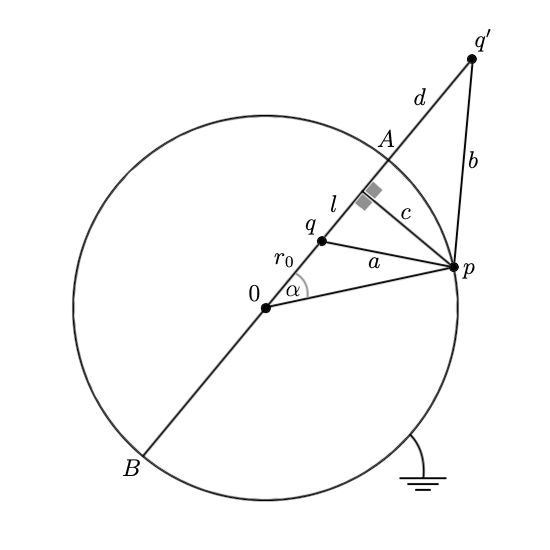
\includegraphics[width=0.5\textwidth]{immagini/caricaimmagine}
\end{center}

Per motivi di simmetria, la carica immagine giace sulla retta che collega 0 e $q$.

Potenziale in $p$:
\begin{equation}
\phi = \frac{q}{a}+\frac{q'}{b} \overset{!}{=} 0
\label{A1}
\end{equation}

prendi $p=A$:
\begin{equation}
\frac{q}{R-r_0} + \frac{q'}{d}=0
\end{equation}
\[
\Rightarrow \frac{q'}{q}=-\frac{d}{R-r_0}
\]

$p=B$:
\begin{equation}
\frac{q}{R+r_0}+\frac{q'}{d+2R}=0
\end{equation}
\[
\Rightarrow \frac{q'}{q}=-\frac{d+2R}{R+r_0}
\]
\[
\Rightarrow \frac{d}{R-r_0}= \frac{d+2R}{R+r_0}
\]
\[
\Rightarrow d(R+r_0)=(d+2R)(R-r_0)
\]
\[
\Rightarrow dR + dr_0 = dR - dr_0 + 2R^2 - 2Rr_0
\]
\begin{equation}
\Rightarrow d=\frac{R(R-r_0)}{r_0}
\end{equation}
e quindi
\begin{equation}
q' = -\frac{dq}{R-r_0} = -\frac{q}{R-r_0}\frac{R(R-r_0)}{r_0}=-\frac{qR}{r_0}
\label{A5}
\end{equation}

Verifichiamo che la \eqref{A1} vale $\forall p$:
\[
\eqref{A1}\Leftrightarrow \frac{q'}{q} = -\frac{b}{a} \overset{\eqref{A5}}{=} -\frac{R}{r_0} \Leftrightarrow \frac{b}{a}=\frac{R}{r_0}
\]
Calcolo l'angolo $\alpha$: 
\[
a^2=r_0^2 + R^2 - 2r_0 R\cos\alpha
\]
\[
\Rightarrow \cos\alpha =\frac{r_0^2 + R^2 - a^2}{2r_0R}
\]
D'altra parte: 
\[
\cos\alpha=\frac{r_0+l}{R}
\]
\[
\Rightarrow \frac{r_0+l}{R}=\frac{r_0^2 +R^2 - a^2}{2r_0 R}
\]
\[
\Rightarrow l=\frac{-r_0^2 + R^2 - a^2}{2r_0}
\]
\[
c^2=R^2 - (r_0+l)^2 
\]
\[
c^2=b^2 - (d +R-r_0 -l)^2 = b^2 -(d+R)^2 - (r_0+l)^2 + 2(d+R)(r_0+l)
\]
\[
\Rightarrow R^2 = b^2 - \underbrace{(d+R)^2}_{\frac{R^4}{r_0^2}} + 2 \underbrace{(d+R)}_{\frac{R^2}{r_0}} \underbrace{(r_0+l)}_{\frac{r_0^2 + R^2 - a^2}{2r_0}}=
\]
\[
= b^2 - \frac{R^4}{r_0^2} + \frac{R^2}{r_0^2}(r_0^2 + R^2 - a^2)
\]
\[
\Rightarrow \frac{R^2}{r_0^2}a^2 = b^2 \Leftrightarrow \frac{b}{a}=\frac{R}{r_0} \qquad \blacksquare
\]

\end{document}